%% ----------------------------------------------------------------
%% Thesis.tex -- MAIN FILE (the one that you compile with LaTeX)
%% ---------------------------------------------------------------- 

% Set up the document
\documentclass[a4paper, 12pt, oneside]{Thesis} % Use the "Thesis" style, based on the ECS Thesis style by Steve Gunn
\graphicspath{Figures/} % Location of the graphics files (set up for graphics to be in PDF format)
\usepackage{adjustbox}
% Include any extra LaTeX packages required
\usepackage[square, numbers, comma, sort&compress]{natbib} % Use the "Natbib" style for the references in the Bibliography
\usepackage{verbatim} % Needed for the "comment" environment to make LaTeX comments
\usepackage{vector} % Allows "\bvec{}" and "\buvec{}" for "blackboard" style bold vectors in maths
\usepackage{qtree}

%\usepackage[lofdepth=1,lotdepth]{subfig}
%\usepackage{caption}
%\usepackage[list=false,listformat=simple]{subcaption}
\usepackage{subfig}
\usepackage{subcaption}
\usepackage{algorithmicx}
\usepackage{algpseudocode}
%\usepackage{titlepic}
%\usepackage{graphicx}
\hypersetup{urlcolor=blue, colorlinks=true} % Colours hyperlinks in blue, but this can be distracting if there are many links.
%\usepackage{polski}

\usepackage[utf8]{inputenc}
%% ----------------------------------------------------------------

\begin{document}


%\frontmatter % Begin Roman style (i, ii, iii, iv...) page numbering

% Set up the Title Page
\begin{center}


\begin{figure}
\centering

\includegraphics{Figures/logo.jpg}
\end{figure}

\vspace*{20mm}

\Huge
\textbf{MASTER THESIS} \\
\Large
by Adrian Szymczak\\

\end{center}

\title {Documents Clustering:\\ A Modern Approach}
%\titlepic{
\includegraphics{Figures/logo.jpg}}
\authors {\texorpdfstring
 {\href{your web site or email address}{Adrian Szymczak}}
 {Adrian Szymczak}
 }
\addresses {\groupname\\\deptname\\\univname} % Do not change this here, instead these must be set in the "Thesis.cls" file, please look through it instead
\date {September 2016}
\subject {}
\keywords {}

\maketitle
%% ----------------------------------------------------------------

\setstretch{1.3} % It is better to have smaller font and larger line spacing than the other way round

% Define the page headers using the FancyHdr package and set up for one-sided printing
\fancyhead{} % Clears all page headers and footers
\rhead{\thepage} % Sets the right side header to show the page number
%\lhead{} % Clears the left side page header

\pagestyle{fancy} % Finally, use the "fancy" page style to implement the FancyHdr headers

%% ----------------------------------------------------------------
% Declaration Page required for the Thesis, your institution may give you a different text to place here
\Declaration{

\addtocontents{toc}{\vspace{1em}} % Add a gap in the Contents, for aesthetics

I, Adrian Szymczak, declare that this thesis titled, `Documents Clustering:\\ A Modern Approach' and the work presented in it are my own. I confirm that:

\begin{itemize} 
\item[\tiny{$\blacksquare$}] This work was done wholly or mainly while in candidature for a research degree at this University.

\item[\tiny{$\blacksquare$}] Where I have consulted the published work of others, this is always clearly attributed.
 
\item[\tiny{$\blacksquare$}] Where I have quoted from the work of others, the source is always given. With the exception of such quotations, this thesis is entirely my own work.
 
\item[\tiny{$\blacksquare$}] I have acknowledged all main sources of help.
 
\item[\tiny{$\blacksquare$}] Where the thesis is based on work done by myself jointly with others, I have made clear exactly what was done by others and what I have contributed myself.
\\
\end{itemize}
 
 
Signed:\\
\rule[1em]{25em}{0.5pt} % This prints a line for the signature
 
Date:\\
\rule[1em]{25em}{0.5pt} % This prints a line to write the date
}
\clearpage % Declaration ended, now start a new page

%% ----------------------------------------------------------------
% The "Funny Quote Page"
%\pagestyle{empty} % No headers or footers for the following pages

%\null\vfill
% Now comes the "Funny Quote", written in italics
%\textit{``Write a funny quote here.''}

%\begin{flushright}
%If the quote is taken from someone, their name goes here
%\end{flushright}

%\vfill\vfill\vfill\vfill\vfill\vfill\null
%\clearpage % Funny Quote page ended, start a new page
%% ----------------------------------------------------------------

% The Abstract Page
\addtotoc{Abstract} % Add the "Abstract" page entry to the Contents
\abstract{
\addtocontents{toc}{\vspace{1em}} % Add a gap in the Contents, for aesthetics

John Naisbitt wrote in his book Megatrends from 1982 “We are drowning in information but starved for knowledge.” Trying to induct meaning from exponentially growing amount of data becomes more and more challenging and makes it easier to get lost in unstructured noise. It is widely known that structuring information enhances perception and making sense of data. In order to understand data better human brains group objects and generalize. As with many other tasks, machine support has proven to work efficiently and there has been proposed great deal of methods performing clustering algorithmically on computers. 

Artificial intelligence and machine learning experts classify clustering as sub-task of unsupervised learning. Author focused on investigating domain of documents clustering with special regard to search results clustering and modern methods making use of advanced natural language processing techniques and external knowledge sources from which can be inferred information about semantic relations in text.

Keywords: document clustering, search results clustering, text clustering, cluster analysis, semantic information, reproducible research
}

\clearpage % Abstract ended, start a new page
%% ----------------------------------------------------------------

\setstretch{1.4} % Reset the line-spacing to 1.3 for body text (if it has changed)

% The Acknowledgements page, for thanking everyone
\acknowledgements{
\addtocontents{toc}{\vspace{1em}} % Add a gap in the Contents, for aesthetics

I would like to thank:

My supervisor dr hab. inż. Mikołaj Morzy for extensive support and inspiration during writing thesis and studies.

My family for unconditional support, dearest parents Agnieszka and Remigiusz, beloved Magdalena and especially my brother Jarek for guidance and mentoring reaching far beyond studies.

People who contributed to this thesis by sharing their thoughts, references to articles and valuable advice: Dawid Weiss and especially Stanisław Osiński - authors of Carrot and Lingo, Marek Kozłowski and Wojciech Stokowiec - from National Information Processing Institute and Jan Mizgajski.

My friends without whom studying would not be equally valuable, pleasant and meaningful, especially: Krzysztof Lewiński, Andrzej Nowicki, Michał Robaczyk, Arkadiusz Rusin, Bartosz Woźniak, Piotr Jakubowski, Kamil Pajdzik, Adam Popiołek, Iwo Błądek, Konrad Miazga, Jakub Lewiński, Jakub Kędzierski, Mateusz Dembski, Mateusz Kurek and Michał Tomczyk.
}
\clearpage % End of the Acknowledgements
%% ----------------------------------------------------------------

\pagestyle{fancy} %The page style headers have been "empty" all this time, now use the "fancy" headers as defined before to bring them back


%% ----------------------------------------------------------------
%\lhead{\emph{Contents}} % Set the left side page header to "Contents"
\tableofcontents % Write out the Table of Contents

%% ----------------------------------------------------------------
%\lhead{\emph{List of Figures}} % Set the left side page header to "List if Figures"
 %\listoffigures % Write out the List of Figures

%% ----------------------------------------------------------------
%\lhead{\emph{List of Tables}} % Set the left side page header to "List of Tables"
 %\listoftables % Write out the List of Tables

%% ----------------------------------------------------------------
\setstretch{1.5} % Set the line spacing to 1.5, this makes the following tables easier to read
\clearpage % Start a new page
%% \lhead{\emph{Abbreviations}} % Set the left side page header to "Abbreviations"
\listofsymbols{ll} % Include a list of Abbreviations (a table of two columns)
{
\textbf{Acronym} & \textbf{W}hat (it) \textbf{S}tands \textbf{F}or \\
\textbf{AMBIENT} & \textbf{AMBI}guous \textbf{ENT}ries \\
\textbf{AMI} & \textbf{A}djusted \textbf{M}utual \textbf{I}nformation \\
\textbf{ARI} & \textbf{A}djusted \textbf{R}and \textbf{I}ndex \\
\textbf{DC} & \textbf{D}ocument \textbf{C}lustering \\
\textbf{ESA} & \textbf{E}xplicit \textbf{S}emantic \textbf{A}nalysis \\
\textbf{JI} & \textbf{J}accard \textbf{I}ndex \\
\textbf{MORESQUE} & \textbf{MORE} \textbf{S}ense-tagged \textbf{QUE}ries \\
\textbf{NLP} & \textbf{N}atural \textbf{L}anguage \textbf{P}rocessing \\
\textbf{NLTK} & \textbf{N}atural \textbf{L}anguage \textbf{T}oolkit \\
\textbf{ODP} & \textbf{O}pen \textbf{D}irectory \textbf{P}roject \\
\textbf{POS} & \textbf{P}art \textbf{O}f \textbf{S}peech \\
\textbf{SRC} & \textbf{S}earch \textbf{R}esults \textbf{C}lustering \\
\textbf{WSI} & \textbf{W}ord \textbf{S}ense \textbf{I}nduction \\
}

%% ----------------------------------------------------------------
%\clearpage % Start a new page
%\lhead{\emph{Physical Constants}} % Set the left side page header to "Physical Constants"
%\listofconstants{lrcl} % Include a list of Physical Constants (a four column table)
%{
% Constant Name & Symbol & = & Constant Value (with units) \\
%Speed of Light & $c$ & $=$ & $2.997\ 924\ 58\times10^{8}\ \mbox{ms}^{-\mbox{s}}$ (exact)\\

%}

%% ----------------------------------------------------------------
%\clearpage %Start a new page
%\lhead{\emph{Symbols}} % Set the left side page header to "Symbols"
%\listofnomenclature{lll} % Include a list of Symbols (a three column table)
%{
% symbol & name & unit \\
%$a$ & distance & m \\
%$P$ & power & W (Js$^{-1}$) \\
%& & \\ % Gap to separate the Roman symbols from the Greek
%$\omega$ & angular frequency & rads$^{-1}$ \\
%}
%% ----------------------------------------------------------------
% End of the pre-able, contents and lists of things
% Begin the Dedication page

\setstretch{1.3} % Return the line spacing back to 1.3

%\pagestyle{empty} % Page style needs to be empty for this page
%\dedicatory{For/Dedicated to/To my\ldots}

%\addtocontents{toc}{\vspace{2em}} % Add a gap in the Contents, for aesthetics
%\mainmatter	
\lhead{\leftmark}

 % Introduction

%% ----------------------------------------------------------------
 % Begin normal, numeric (1,2,3...) page numbering
\pagestyle{fancy} % Return the page headers back to the "fancy" style

% Include the chapters of the thesis, as separate files
% Just uncomment the lines as you write the chapters

\chapter{Introduction} Internet is by far single largest information source worldwide. Exponential growth of amount of electronic documents, especially in the era of the Internet, results in need for effective methods to organize such vast amount of information. Whether these are news articles, Facebook posts, tweets, websites or just snippets returned as search results by popular engine, many various topics and concepts mix in them and result in confusion. Identifying these topics and concepts, together with presentation of corresponding to them documents, is crucial for effective data exploration. In computer science, clustering is technique to achieve it, and using it to enhance search functionality was subject of thorough investigation and also is the main focus of this thesis. 

Ambiguities in queries are often introduced by using words with many possible meanings like for instance tiger, which might refer to animal, river, famous golf player Tiger Woods or German tank. Because there are many possible meanings of given word and users tend to submit short queries either because of unawareness or laziness, resolving uncertainties is crucial for satisfying information need.

Thanks to possibility of processing huge text corpora and external data sources it is natural to address problem of clustering not only with use of traditional mathematical, data oriented methods but naturally by trying to determine meaning of words from global semantic context. Clustering problem can be addressed in various ways and because it does not have one proper solution many areas of focus are emphasised by particular algorithms. Author proposes novel algorithm to search result clustering based on word semantic similarities using automatic discovery of word senses from raw text. Exact plan and planned original contributions will shed more light on briefly introduced subject and thesis.

\section{Scope of work and original contributions} Additionally to conducting in depth literature survey about clustering text documents and search results with special regard to those making use of external semantic knowledge sources and relatedness between words, two components are author's main original contributions:

\begin{itemize}
 \item Proposing novel documents clustering algorithm (Chapter 10) using external knowledge sources for semantic relations and advanced Natural Language Processing techniques (Chapter 5). Additionally evaluating proposed algorithm (Chapter 11) using various measures (Chapter 4) on chosen datasets (Chapter 6), following reproducible research rules (Chapter 8), using proper tools and techniques (Chapter 9) and making use of vast majority of theory discussed in thesis (remaining Chapters).
 
 \item Formulating reproducible research rules (Chapter 8) recommended by author after observing way of conducting research in documents clustering domain with applications reaching far beyond its scope. Additionally covering technicalities of conducted research and applied engineering techniques (Chapter 9), emphasising their usage for sake of successfully implementing mentioned methodology (Chapter 8).
\end{itemize}

\clearpage

\section{Thesis structure} Thesis is composed of 12 chapters focusing on following subjects:
\begin{itemize}
 \item Chapter 1 - Presenting field of study and defining what will be done as author's original contribution to it. Clearly defining targets which ought to be achieved, and topics to be covered in each chapter.
 \item Chapter 2 - Conducting in depth literature survey about evolution of domain with distinction to algorithms families.
 \item Chapter 3 - Covering the most basic concepts to give foundation for further study in order to understand basic considerations in thesis as well as algorithms investigated during literature study.
 \item Chapter 4 - Discussing large variety of clustering evaluation methods with use of numerous measures.
 \item Chapter 5 - Presenting Natural Language Processing techniques used in documents clustering with special regard to time consumption and potential of improving clustering results.
 \item Chapter 6 - Studying the most common datasets with distinction between datasets used in search results clustering and classic classification problems (and how to adjust them).
 \item Chapter 7 - Discussing knowledge sources and their characteristics as well as techniques to infer semantic relatedness.
 \item Chapter 8 - Formulating reproducible research rules recommended by author.
 \item Chapter 9 - Covers technicalities of conducted research and applied engineering techniques.
 \item Chapter 10 - Presenting novel documents clustering algorithm being major original contribution using external knowledge sources for semantic relations and advanced Natural Language Processing techniques.
 \item Chapter 11 - Summing up and discussing results.
 \item Chapter 12 - Formulating conclusions followed by recommendations for prospective further work.
\end{itemize}

\chapter{Background}

\section{Clustering} Clustering is unsupervised learning task, that based on features and information about objects, proposes their natural grouping. This exploratory data mining technique aims to achieve such division, that objects from the same cluster are as similar as possible to each other, and as dissimilar as possible to objects from other clusters. Thanks to it, reasoning about objects is significantly simplified and understanding non obvious, often hidden structures is possible. Document clustering objectives are twofold:
\begin{enumerate}
\item create clusters and assign documents to them, with regard to algorithm steps and potential objective functions
\item provide informative labels of discovered clusters
\end{enumerate}

Division of objects into clusters has many possible success indicators and there is not one clear solution. Conventional algorithms focus on first objective, when others try to address later and additional, more specific objectives. There are many different types of clustering. Some methods assume that document can be assigned only to one cluster (hard), others that to many different clusters (soft). Another distinction can be made by assuming underlying distribution of data and trying to fit objects into it (probabilistic), or by grouping with no such assumption and generating distribution by oneself (generative). Further division can be made by going into more details of the way documents are processed, like distributed vs centralized, or centroid vs distribution vs density based etc.

\section{Cluster Labeling} Conventional clustering algorithm focus on first objective and like the most recognizable clustering algorithm k-means, are not capable of producing meaningful cluster labels. If cluster labels are present at all, they often contain just pieces of text which does not project any understandable, cluster-content related. 

Presentation of informative cluster labels, has potential to trigger corresponding concept in the user’s mind and project cluster content in an understandable form. It is serious issue in many domains where clustering can be applied, and in certain domains like search results clustering it is crucial. When going through ranked list of search results, users can easily narrow down focus to the most relevant clusters, representing subset of documents which fully meets initial information need.

\section{Search Results Clustering} Search Results Clustering (SRC) is subdomain of documents clustering which characteristic is presence of query constraint and focus on clustering short documents with regard to presented, often ambiguous, topics quickly. Classic search engines try to address similar problem and are often used hand in hand, because both after being provided with particular query from user, then try to determine which results are the most relevant. Users unfortunately due to being unaware or potentially lazy, provide very short, maximum a few words long queries, which in result are ambiguous what naturally leads to yielding different documents spanning through large variety of topics. In effect many documents are not being discarded from results as irrelevant, despite likely not satisfying information need.

Having particular piece of information in mind and expressing it clearly in query is very rare. Vast majority of search queries is exploratory, so user has just brief idea about what might be a result, but lack specific expectations, what obviously gives huge field for research. There are different families of algorithms trying to perform clustering task effectively in these conditions. They are discussed in details in following chapter. Worth mentioning now is however, that set of cluster labels optimally should provide concise topic overview. Necessity of a informative cluster label goes hand in hand with semantic relatedness, hence cluster labels are very important for discussed subdomain. Disambiguation of search results can be achieved thanks to statistical inference and sophisticated algorithms, among them clustering - what is naturally the most interesting from thesis perspective.

\section{Challenges in Clustering} Clustering has to address important challenges, because many factors have to be taken into consideration to create what can be considered "good" clustering. Additionally when focusing on Search Result Clustering (SRC), extra challenges arise, and there are more requirements to be fulfilled \cite{weiss2002introduction}. Unlike in classic Documents Clustering (DC), in which full text is taken into consideration, SRC has to deal with text snippets. Because snippets are usually just few sentences long, what might be very small part of original text, a lot of meaning is lost introducing noise, especially from small samples.

DC algorithms should address following challenges:
\begin{itemize}
\item choosing appropriate representation model and similarity measure
\item adding new elements to clusters without need for re-clustering (being incremental / on-line)
\item implement policy of handling outliers properly
\item assuming predefined number of clusters or determining them on the fly
\item processing in distributed or centralized manner
\item scalability in face of large amount of documents or features
\end{itemize}

SRC algorithms should address additionally following challenges:
\begin{itemize}
    \item linear or logarithmic time complexity as time is crucial for them
    \item good results given input data insufficient to deduct only from it
    \item producing intuitive cluster labels, supporting users' understanding of clusters' nature
    \item potentially overlapping clusters for topics mixture
    \item distinction on snippet, URL address and title
    \item disambiguation through word sense induction and potentially preprocessing external knowledge sources
\end{itemize}

\section{Clustering Applications} Clustering has wide range of applications. Because people can take limited numbers of parameters into consideration, assistance in analysis of multidimensional data, otherwise not comprehensible by humans, is extremely valuable. Clustering not only enhances exploratory analysis in support of decision making, but also improves visualization.

Among the most prominent fields, in which clustering has been successfully adapted are: text mining, image processing, medicine, biology and business. Because thesis will focus on text mining, applications from other fields will be only briefly discussed. Market segmentation is the most obvious business application, because for instance finding groups of customers exposing similar behaviour or characteristic, helps to formulate pricing strategy or create advertising campaign which targets particular cluster of users. Taxonomy of species can be created based on living organism's features. In medicine, processing brains or eyes scans assisted with information about patients' history, age, gender etc. helps to understand and visualise results of research and nature of illness or defects. Interesting application of documents clustering is supporting lawyers in process of knowledge discovery in legal documents \cite{kozlowski2015law}. 

Especially with regard to this thesis, clustering can help resolve ambiguities in search results, what will be discussed in following part of thesis below.

\section{SG and CBOW model}  Plain text documents have to be mathematically modelled in order to allow performing clustering by vast majority of methods as they assume particular representation model of input documents. Among the most popular representations are vector space model, probabilistic topic models and graph model. Discussed further will be skip-gram model and graph model because of being used in thesis. Used for word2vec purposes Skip-gram (SG) can be seen as predicting the context given a word, whereas  Continuous Bag-of-Words (CBOW) can be seen as predicting the word given its context.

For CBOW size of window in settings influences number of words used and for SG how far forward and backward to look for context words to predict. According to author of SG \cite{guthrie2006closer} in comparison with CBOW it works well with small amount of the training data and represents well even rare words or phrases. 

Skip-gram (SG) illustrated at figure~\ref{fig:skip} on page~\pageref{fig:skip} and Continuous Bag-of-Words (CBOW) model is illustrated at figure~\ref{fig:cbow} on page~\pageref{fig:cbow}. Both are are compared in \cite{guthrie2006closer} and in short both describe the way in which the neural network learns underlying word representations for each word.

For instance the sentence "I love you my dear pizza!" becomes:
\begin{itemize}
\item CBOW (3-grams): "I love you", "love you my", "you my dear", ...
\item SG (1-skip 3-grams): "I love you", "I love my", "love you my", "love you dear", ... 
\end{itemize}
it is crucial that in SG "I love my" skips over "you"

\begin{figure}[h]
  \centering
  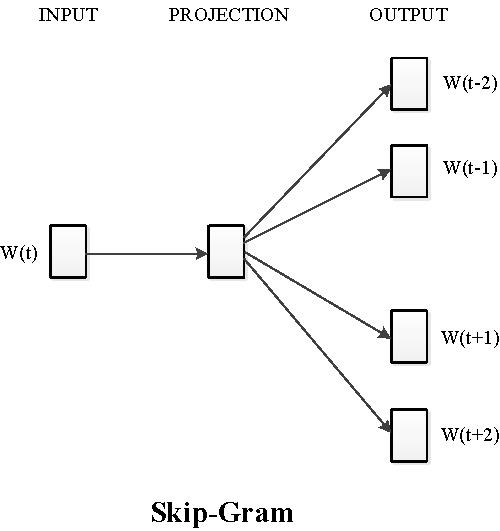
\includegraphics[width=.5\linewidth]{Figures/skip.png}
  \caption{Skip-Gram model}
  \label{fig:skip}
\end{figure}

\begin{figure}[h]
  \centering
  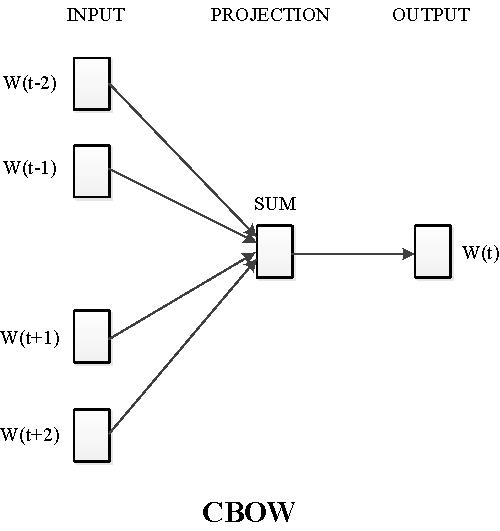
\includegraphics[width=.5\linewidth]{Figures/cbow.png}
  \caption{Continuous Bag-of-Words model}
  \label{fig:cbow}
\end{figure}

\chapter{Related work} Search Result Clustering (SRC) algorithms can be classified into three types: description-centric, data-centric and description-aware \cite{carpineto2009survey}. Additionally semantically enhanced approaches, using word sense induction, are gaining popularity. Quick discussion of related work done in a field with regard to these categories is presented below.

\section{Data-centric algorithms} Data-centric algorithms heavily focus on clustering process and are represented by many traditional clustering algorithms (hierarchical, fuzzy, density-based and partitioning). They treat search results clustering problem in similar manner to classic clustering problem, hence these algorithms can be applied not only in text domain. 

Data-centric algorithms find the best solution based on data usually represented as mathematical model. In text domain the most popular one is Vector Space Model (VSM) \cite{salton1975vector}. Major disadvantage of heavy data focus is producing often meaningless, poor quality cluster labels, that do not describe well clusters' content.

There are many various methods representing data-centric algorithms category, although discussion will focus on couple of the most representative. One approach is hierarchical clustering, in which algorithms generate dendogram (tree of clusters), using one of three similarity measures between clusters: single link, complete link and average link. The best results were achieved by algorithm UPGMA \cite{jain1988algorithms}, although hierarchical algorithms in general perform poorly on documents clustering and have $O(N^3)$ complexity. 

Worth mentioning is also pioneer example of using clustering to help browsing documents by two step method Scatter Gather \cite{cutting1992scatter}, which firstly clusters documents and shows results to the user (Scatter), who then appoints the most appropriate cluster, which will be used in the next iteration for re-clustering (Gather). 

Another approach in partitioning clustering is represented by algorithms, which \cite{jain1988algorithms}, \cite{jain1999data} perform an initial division of the data in the clusters, and only then move objects from one cluster to another based on optimization of a predefined criterion or objective function. The most representative algorithms that use this technique are: k-means, k-medoids, and Expectation Maximization.

The k-means algorithm is definitely the most popular and easy to implement. For finding local optimum its time complexity is $O(nkid)$, what in practical applications often means $O(n)$. Version of algorithm adapted for finding global optimum is however NP-hard. Moreover for instance k-means is sensitive to outliers and can produce only clusters that are hyper spherical, selection of the initial centroids often leads to different results and predefined number of clusters has to be provided. As alternative bisecting k-means algorithm \cite{li2008text} was proposed in which hierarchical and partitioning methods are mixed for producing better results than the UPGMA and k-means.

As mentioned data-centric algorithms struggle with producing good quality cluster labels and usually address this problem separately as independent step of clustering algorithm. One approach is to use keywords from text with regard to their frequency in given documents or make use of probability theory and analyze distributions. More promising however is generation of cluster labels using external knowledge sources. For instance titles and categories of Wikipedia articles were used in \cite{carmel2009enhancing}. 

Closing gap between creation of quality clustering with regard to data and producing meaningful cluster labels, is relevant enough to create dedicated class of algorithms, which puts more emphasis on addressing labels problem.

\section{Description-aware algorithms} This family of algorithms is sometimes joined with description-centric algorithms, because it emphasises creation of high quality and meaningful cluster labels by selecting one or more features to focus on, at cost of decrease in classic data focused clustering metrics. Difference is how much stress is put on description creation and also because description-aware algorithms were implemented before fully description-centric ones. Main issue of description-aware algorithms is that the cluster labeling process dominates overall clustering process sacrificing performance of data related clustering measures.

The most widely known representative of this group is Suffix Tree Clustering (STC) \cite{zamir1998web} algorithm, which uses phrase model for documents representation. By using common phrases from documents it incrementally creates labels easily interpretable by users. It was investigated extensively and improved both in terms of performance and resources consumption. Alternative option making use of user queries was proposed at SnakeT \cite{ferragina2008personalized}. 

\section{Description-centric algorithms} Description-centric algorithms are designed specifically for clustering web documents. They not only focus on meaningful cluster labels but also strive to provide high quality clusters. The most widely known examples in this category are:

SHOC \cite{zhang2004semantic} (Semantic, Hierarchical, Online Clustering) which is based on LSI and frequent phrases and improves STC algorithm discussed in previous section.
LINGO \cite{osinski2004lingo} used in the Carrot2 web clustering engine, based on complete phrases and LSI with Singular Value Decomposition (SVD). It first tries to discover descriptive cluster labels and after this organizes the documents into appropriate clusters.
Full-Subtopic Retrieval with Keyphrase-Based Search Results Clustering (KeySRC) \cite{bernardini2009full} is based, as name suggests, on key phrases extracted from a generalized suffix tree built from the search results. In this algorithm documents are later clustered using hierarchical agglomerative clustering algorithm. 
In \cite{zeng2004learning} problem of documents clustering was approached as a supervised salient phrase ranking problem with use of techniques like linear regression, logistic regression and support vector machines.
Dynamic SVD clustering (DSC) \cite{mecca2007new}, which uses SVD and minimum spanning tree (MST).
CFWS (Clustering based on Frequent Word Sequences) and the CFWMS (Clustering based on Frequent Word Meaning Sequences) algorithms \cite{li2008text} have the text documents represented as frequent word sequences and frequent concept sequences (with use of WordNet). 
FIHC (Frequent Itemset-based Hierarchical Clustering) \cite{fung2003hierarchical}  which is an algorithm that measures the cohesion of a cluster using frequent word sets in a way that the documents in the same cluster share more frequent word sets than those in other groups. 
FTC (Frequent Term- Based Text Clustering) and HFTC (Hierarchical Frequent Term-Based Text Clustering) algorithms \cite{beil2002frequent} use frequent word sets for document representation in clustering of web results and combinations of frequent words (association rules approach) shared in the documents to measure distance in the text clustering process.
Other interesting approaches are STHAC \cite{worawitphinyo2011improving} and CREDO \cite{carpineto2004exploiting}

\section{Semantic-enhanced} This family of algorithms is getting a lot of attention recently and sometimes is mixed with description centric, although should be discussed separately, because novel algorithm proposed in thesis represents this novel approach, based on discovery of word senses automatically from raw text. This way of resolving query ambiguity is called Word Sense Induction (WSI) and algorithms using it have proven to be effective. WSI goes beyond classic syntactic similarity or synonyms and tries to asses word sense from raw texts dynamically creating senses for potential input queries. Logic behind this approach is that quality of clustering suffers if documents in particular cluster share the same terms at syntactic level, but which are semantically different. In the same way documents related semantically might be members of different clusters if decision is made just on term similarity at a syntactic level.

Majority of WSI algorithms make use of knowledge bases and external resources (among them web directories Wikipedia, Open Data Project (DMOZ), DBPedia, and search engine query logs, crawling web sites dump, TAGME etc.) in order to construct co-occurences graph of terms and process it to acquire different senses of ambiguous words. Then they perform clustering of search result base on semantic similarity between terms using various evidences like text titles, snippets or full documents returned by text engine. Discovery of word senses is crucial to algorithm as well as knowledge base used and implementation detail depend on specific algorithm characteristics. Methods which are especially promising in this family are discussed below.

HyperLex \cite{veronis2004hyperlex} is pioneer effective algorithms based on identification of hubs representing specific meaning in co-occurence graphs.

Squares, Triangles, and Diamonds (SquaT++) \cite{di2013clustering} is an algorithm that integrates two graph patterns previously exploited in the literature, namely, squares and triangles, with a novel pattern called diamond.

Balanced Maximum Spanning Tree Clustering (B-MST) is WSI enhanced algorithm, that aims at balancing the number of co-occurrences in each sense cluster.

Chinese Whispers \cite{biemann2006chinese} is different from others as it is randomized algorithm. It partitions nodes of graph by transferring iteratively given mainstream message, which might be for instance word sense, to nodes in neighbourhood. 

Curvature clustering calculates participation words in complete graphs with three nodes and takes their ratio into consideration while producing solution.

More recently \cite{wahid2013exploiting} algorithm QSC was proposed, that exploits user query as well as semantic and syntactic features of a document making use of Wikiminer \cite{milne2013open} for word disambiguation. 

Another approach represents algorithm Topical \cite{scaiella2012topical} which treats problem of clustering web results in similar manner as labeling clustering nodes of a graph of topics. Tagme annotations replace the traditional bag of words paradigm. Topics are Wikipedia pages identified by a topic annotator and edges of the graph denote the relatedness of these topics. 

In \cite{kozlowskiweb} Bisecting, K-Means, STC and Lingo were enriched with semantic features from BabelNet (disambiguated synsets, semantic edges and categories and glosses describing synsets). Unfortunately extensive investigation was not possible due to limitations of BabelNet API and results were tested only on AMBIENT dataset, but even so obtained results did not improve results almost at all (about 1\%).

\section{Clustering as objective optimization} Stochastic discrete optimization algorithm can provide good approximations to the optimal solution for the search results clustering (SRC) problem. Recently approach named Clustering Ensembles is getting a lot of attention, because it produces better results by combining results of different clustering methods \cite{vega2011survey}. In general, clustering ensemble methods formulate clustering as single objective optimization problem, however according to recent studies, using two or more objectives generates better results \cite{strehl2002cluster}. In clustering ensemble methods firstly candidate clustering solutions are generated, and then from them single solution is obtained (for instance median), usually with use of similarity criterion (for instance maximum average similarity to previously generated solutions). 

A comprehensive analysis of multi-objective approaches can be found in \cite{nanda2014survey}. One of popular cluster ensemble methods is MOCK \cite{handl2013evidence}, which is based on modified version of SPEA-II (Strength Pareto Evolutionary Algorithm) algorithm and two objective functions: connectedness and compactness of the cluster. Another popular approach is MMOEA \cite{wahid2015multi} based on NSGA-II algorithm (Non-dominated Sorting Genetic Algorithm). Generally majority of multi-objective clustering ensembles focus on minimizing intra-cluster variance.

Moreover another algorithm OPTIMSRC (OPTImal Meta Search Results Clustering) \cite{carpineto2010optimal} uses labels generated by other algorithms like Lingo or STC in order to match most appropriate labels with the generated clusters.

\chapter{Clustering evaluation methods} As there is not one "good" clustering problem solution, great deal of measures were proposed to evaluate the results. Many algorithms try to be well balanced when others target particular measure. Discussion of the most widely used ones follows.

\section{Unsupervised clustering evaluation} There are several methods taking into account clusters structure without their interpretation and actual content. In this section we describe such methods, however algorithm proposed in thesis does not have defined similarity measure between documents and also similarity between clusters and can not be evaluated with them.

\subsection{Silhouette Coefficient} Silhouette Coefficient was proposed in \cite{rousseeuw1987silhouettes} as a graphical display for partitioning techniques. It shows which objects seem to belong to cluster and which ones tend to be between two or more clusters. The measure for each observation is then aggregated by averaging into the coefficient of the cluster and the total coefficient of clustering results.

Silhouette coefficient of a certain document is given with the following formula:
$$ s(i) = \frac{b(i) - a(i)}{max\{a(i), b(i)\}} $$

Where:
\begin{itemize}
\item $a(i)$ stands for dissimilarity of document $i$ to its own cluster defined as an average distance to all the data points within the cluster (for cluster size one $s(i) = 0$)
\item $b(i)$ is similar to $a(i)$, however analysed cluster is the cluster with lowest average dissimilarity (distance) to the document (other than its own cluster)
\end{itemize}

Silhouette coefficient typically ranges from zero, when record is on a boundary of two clusters, to one, when record is identical to other records in cluster.

It is theoretically possible that Silhouette coefficient is below zero (not lesser than $-1$), however such values would indicate that there is a smaller dissimilarity measure for a record to another cluster than to its own.

\subsection{Dunn Index} Dunn Index \cite{dunn1973fuzzy}, is defined as:
$$ DI_m = \frac{\underset{1 \leq i \le j \leq m}{min} \delta(C_i, C_j)}{\underset{1 \leq k \leq m}{max} \Delta_k} $$

where:
\begin{itemize}
\item $m$ is a number of clusters
\item $C_i$ is a cluster
\item $\delta$ is a measure of dissimilarity between the clusters, defined in a custom manner (average, maximum, etc.)
\item $\Delta_k$ is an aggregation, for cluster $C_k$, of intracluster distance, also in a custom manner (average, minimum, distances of all the points from cluster center, etc.) 
\end{itemize}

Dunn Index is a pesimistic measure, as it is sufficient that one of the clusters is badly created to cause the whole measure to indicate the poor quality of the clustering.

\subsection{Davies–Bouldin Index} Davies–Bouldin Index \cite{davies1979cluster} clustering quality measure is similarly like Dunn Index a pesimistic measure of clustering quality.

Defining the following concepts:
\begin{itemize}
\item $S_i$ scatter of the cluster, the lower the better
\item $M_{i,j}$ separation of cluster $C_i$ and $C_j$, the higher the better
\end{itemize}

An measure $R_{i, j}$ was introduced as:
$$ R_{i,j} = \frac{S_i + S_j}{M_{i,j}} $$

To define:
$$ D_i = \underset{j \neq i}{max} R_{i,j} $$

Davies–Bouldin Index for $N$ clusters is then given as:
$$ DB = \frac{1}{N} \sum_{i=1}^{N} D_i $$

\section{Supervised clustering evaluation, relevant} In this section we describe evaluation methods. The evaluation is performed as a comparison with regard to human user interpretation or so called gold standard. The gold standard is a perfect / desired way of clustering the documents (e.g. an actual division of documents into categories). Mutual Information, Rand Index, Jaccard and \mathit{F-measure} are evaluated. Moreover extensive analysis of results obtained by these measures and various b-cube adjusted measures with regard to different scenarios can be found at \cite{moreno2015adapted}.

\subsection{Mutual Information}\label{section:MutualInformation} Mutual information reflects the amount of information that is shared between division of documents into clusters and classes. Its main advantage as a measure is that it can be used also for cases in which the number of clusters differs from number of classes. It is defined as \cite{andrews2007recent}:

$$ MI = \sum_{i,j} P(i,j)\, log \frac{P(i,j)}{P(i) P(j)} $$

Where:
\begin{itemize}
 \item $P(i)$ is the probability that the document is of class $i$
 \item $P(j)$ is the probability that the document belongs to cluster $j$ 
\end{itemize}

There is no upper bound for mutual information value, hence it is commonly normalized to fall in range $[0, 1]$ in the following manner \cite{strehl2002cluster}:

$$ NMI = \frac{\sum_{i,j} P(i,j)\, log \frac{P(i,j)}{P(i) P(j)}}{\sum_i P(i)\, log P(i)\, \sum_j P(j)\, log P(j)} $$

Finally in thesis results are evaluated with Adjusted Mutual Information (AMI) proposed in \cite{vinh2010information} as an adjustment of the Mutual Information (MI) score to account for chance. It accounts for the fact that the MI is greater for two clustering solutions U and V (real and gold standard) with a larger number of clusters, regardless of whether there is actually more information shared. Permutation of the class or cluster label values does not change AMI value, which in general is given with formula:

$$ AMI(U, V) = \frac{[MI(U, V) - E(MI(U, V))]}{[max(H(U), H(V)) - E(MI(U, V))]} $$

\subsection{Rand Index}\label{section:RandIndex} Rand Index \cite{rand1971objective} is a measure of accordance between two clustering results. Given the clustering resulting in division into clusters $U$ and another division into clusters $V$, and defining:
\begin{itemize}
 \item $N_{11}$ - as a number of document pairs that are in the same cluster in both $U$ and $V$
 \item $N_{10}$ - as a number of document pairs that are in the same cluster in $U$ and in different clusters in $V$
 \item $N_{01}$ - as a number of document pairs that are in different clusters in $U$ and in the same cluster in $V$
 \item $N_{00}$ - as a number of document pairs that are in different clusters in both $U$ and $V$ 
 \item $N$ - a total number of documents in all the clusters

\end{itemize} 

Rand Index is defined as follows:
$$ RI(U, V) = \frac{N_{11} + N_{00}}{N_{11} + N_{10} + N_{01} + N_{00}} = \frac{N_{11} + N_{00}}{\binom{N}{2}} $$

Let $G$ be the gold standard / ground truth of clustering a particular set of documents. In a common setting where clustering result (denoted as $C$) is evaluated based on correct classification of documents, the classification serves as the golden standard and Rand Index is used in similar manner as other measures described in this section and $R(G, C)$ is calculated.

Rand Index is limited to interval $[0, 1]$ but most commonly falls into range $[0.5, 1]$ and therefore an alternative measure called Adjusted Rand Index was proposed \cite{hubert1985comparing}:
$$ ARI(U, V) = \frac{2(N_{00} N_{11} - N_{01}N_{10})}{(N_{00} + N_{01})(N_{01} + N_{11}) + (N_{00} + N_{10})(N_{10} + N_{11})} $$

Such adjusted version is commonly used in algorithms comparison \cite{vinh2010information}.

\subsection{\mathit{F-measure}}\label{section:FMeasure} \mathit{F-measure} is a commonly used metric in Information Retrieval (IR) for aggregating precision and recall. In IR, precision is the proportion of relevant retrieved records from all retrieved records, while recall is proportion of relevant retrieved records from all relevant records.

In clustering setting with classification based evaluation, given that clustering is a series of decisions for each pair of documents, whether to put them in the same cluster or not.

Classic precision and recall formulas are as follows (where $TP$, $TN$, $FP$, $FN$ stand for true positives, true negatives, false positives and false negatives):
$$ precision = \frac{TP}{TP+FN} $$
$$ recall = \frac{TP}{TP+FP}$$

In clustering settings, having a clustering results $C$ and the actual classes used as gold standard $G$, the interpretation is as follows:
\begin{itemize}
 \item $TP$ - a pair of documents is in the same cluster in $C$ and $G$
 \item $FN$ - a pair of documents is in different clusters in $C$ but the same one in $G$
 \item $TN$ - a pair of documents is in different clusters in $C$ and $G$
 \item $FN$ - a pair of documents is in same cluster in $C$ but different clusters in $G$
 \end{itemize}
 
 \mathit{F-measure} is given with formula \cite{andrews2007recent}:
 $$ \text{\mathit{F-measure}} = \frac{(\beta^2 + 1) \cdot precision \cdot recall}{\beta^2 \cdot precision + recall} $$
 
 For $\beta = 1$, \mathit{F-measure} is referred as $F1$.

 There is also an alternation of classic \mathit{F-measure} called b-cubed \mathit{F-measure} defined in  \cite{acharya2014multi}. Moreover \mathit{F-measure} is often calculated differently in various papers what makes it hard to compare results. For instance some papers calculate it as micro averaged, others as macro averaged, and many make modifications and arbitrary adjustments by not taking into consideration clusters with less than 3 elements etc. like for instance in \cite{di2013clustering}.
 
 Another definition of \mathit{F-measure} uses single clusters precision (P) and topics recalled (R) by them as defined in \cite{crabtree2005improving}. Evaluating clustering \mathit{C} against gold standard \mathit{G} is performed as follows:
 
 P determines how accurately clusters in \mathit{C} represent topics in \mathit{G}, whereas recall how accurately topics in \mathit{G} are covered by clusters in \mathit{C}. The majority topic for a cluster $ C_j \in C $ is the topic \mathit{t} for which there exists the maximum number of snippets in $ C_j $ tagged with \mathit{t}.

$$ P(C_j) = \frac{|C_j^t|}{|C_j|} $$

where \mathit{t} is the majority topic in $ C_j $ for a given query, and $ C_j^t $ is the set of snippets in $ C_j $ which are tagged with subtopic \mathit{t} in the gold standard \mathit{G}. The recall of a topic \mathit{t} is, instead, calculated as:

$$ R(t) = \frac{|\cup_{C_j \in C^t}C_j^t|}{n_t} $$

where $ C^t $ is the subset of clusters of \mathit{C} whose majority topic is \mathit{t}, and $ n_t $ is the number of snippets tagged with subtopic \mathit{t} in the gold standard. The total precision and recall of the clustering \mathit{C} are then calculated as:

$$ P = \frac{\sum_{C_j \in C} P(C_j)|C_j|}{\sum_{C_j \in C} |C_j|} $$

$$ R = \frac{\sum_{t \in T} R(t)n_t}{\sum_{t \in T} n_t} $$

where \mathit{T} is the set of subtopics in the gold standard \mathit{G} for the given query. This version is not widely used but might be useful for enabling comparison with paper which investigated many interesting algorithms (unfortunately with many silent assumptions) mentioned above \cite{di2013clustering}. 

\subsection{Jaccard Index}\label{section:Jaccard} Jaccard Index in the context of comparison of the results of clustering \mathit{C} with gold standard \mathit{G} is defined as follows \cite{di2013clustering}:

$$ JI = \frac{TP}{TP + FP + FN} $$

In contrast to Adjusted Rand Index, Jaccard Index completely ignores the true negative values - $TN$, compensating for potential overweighting of usefulness of the information that certain documents are in two different clusters.

For description of the equation, please take a look at \mathit{F-measure} section.

\section{Supervised clustering evaluation, overview}

\subsection{Entropy} Entropy is commonly known as measure of disorder. In a validation of clustering treated as classification settings, entropy has an interpretation of distribution of examples within clusters among classes (aggregated to a single measure proportionally to a cluster size).
As per \cite{andrews2007recent}, entropy is defined as follows:

$$ Entropy = -\frac{1}{log\, k} \sum_j \frac{n_j}{n} \sum_i  P(i,j)\, log P(i,j) $$

Where:
\begin{itemize}
 \item $k$ is the number of clusters
 \item $n$ is the number of documents in total
 \item $n_j$ is the number of documents in $j^{th}$ cluster
 \item $P(i,j)$ is the probability within cluster $j$, that a document from that cluster is of class $i$
\end{itemize}

Entropy is not a reliable measure in case when number of clusters is different than number of classes.

\subsection{Purity} Purity is a simple measure. Its interpretation on single cluster level is that for each cluster it determines what fraction of all the documents in a cluster are from dominant class in that cluster. As a measure for clustering results it is summed among the clusters with weight being proportional to cluster size. Similar as in case of entropy, this measure is not suitable for cases when number of classes differs from number of clusters.

Formula to calculate purity is as follows \cite{andrews2007recent}:
$$ Purity = \sum_i  \frac{n_j}{n}\, \underset{i}{argmax} P(i,j)$$

\subsection{User surveys} As there may be more than one correct division of the documents into clusters (depending on what is taken into account as criteria) - various results could be either useful or not. Further in this chapter we will present the strict, numeric measures for clustering evaluation. We would however like to start with a mention of an interesting approach proposed in \cite{osinski2004lingo}, where users given a certain results of clustering had a task to evaluate whether cluster description was meaningful and the documents assigned to those clusters were logical. Such assessment has a great disadvantage of subjective individual bias, however it is natural, that users for whom the clustering algorithm would be used, are very good judges of its usefulness.

\subsection{Other} Many SRC algorithms take into consideration positions and relevance of returned elements on ranked lists of results. In order to determine diversification measures which are widely used are S-recall@K (Subtopic recall at rank K), which evaluates performance of system based on first K top-ranked results for number of topics of query q, and also S-precision@r (Subtopic precision at recall), which measures the ratio of subtopics covered by minimum set of results at given recall r. Logic behind these measures is that search results list needs to be diverse and top ranked results should represent different senses of the user query.

Alternatively Subtopic Search Length under k document sufficiency $ SSL_k $ metric can be used for checking how easily users can use clustering results. It is defined as the average number of items (cluster labels or search results) that must be checked before finding sufficient number (k) of relevant documents to any of the query subtopics, assuming that both cluster labels and search results are read sequentially from top to bottom, and that only cluster with labels relevant to the subtopic at hand are opened.

\chapter{Natural Language Processing} Possibilities of algorithms treating documents as simply bag-of-words are limited. NLP (Natural Language Processing) techniques greatly influence efficiency and performance of clustering. DC algorithms usually adapt only the most basic methods which are fast and easy to implement, namely tokenization, stemming, normalization and stop words removal. In this chapter we will discuss more advanced techniques as well.

\section{Tokenization and Normalization} Document is made of characters usually fitting into one of four groups - letters, numbers, white-spaces and punctuation signs. As part of preprocessing documents set every single document is transformed into list of tokens referred to as terms or words. It is performed often by removing all numbers and treating punctuation signs and white-spaces as word delimiters. Sometimes all letters are changed to lower-case and characters outside specific alphabet are ignored but it depends from main language of document and applied policy.

Performing normalization has main purpose of transforming tokens into semantically interpretable phrases referred to as types. Synonyms and intelligent processing using word sense induction is far more complex and in case of normalization focus is on not confusing "aren't", "are not" and "arent". Situation can complicate when considering email addresses, URLs, entity names etc. as what is further discussed in dedicated section sometimes tokenization and normalization in special way handles such cases like "Salt Lake City", "Bill Gates" or "Coca-Cola", "co-occurence" etc.

Tokenization strategy should be carefully picked as it is easy to imagine scenario when classic approach is not acceptable. For instance clustering legal documents where numbers might encode personal data, case details etc. have usually high distinctive value and clusters should be constructed around them.

\section{Stemming and Lemmatization} For grammatical reasons words in documents appear in different forms like organize, organizes, and organizing. What is more, there are families of semantically similar words like democracy, democratic, and democratization. It is intuitive that treating such words as one, would be beneficial for processing purposes and for improvement of retrieval performance. Thanks to reducing variants of word to the same root, matches between a query and a document are more frequent. In effect more documents can be returned achieving better recall. Additionally size of distinct terms decreases, allowing to save space when storing documents and lowering size of index.

One way of doing it is by performing stemming, which refers usually to removing suffix or prefix of word, depending on language of text. Together with applying specific rules of the most popular English language stemming Porter's algorithm \cite{porter1980algorithm} satisfactory results are produced in timely manner. 

Another possibility is lemmatization, which is more sophisticated and time consuming method. It makes use of vocabulary and morphological analysis of words, aiming to yield just the base or dictionary form of a word. For token token "saw", stemming could return just "s", whereas lemmatization would possibly return either "see" or "saw" depending on whether the use of the token was as a verb or a noun.

\section{Stop Words Removal} There are words that occur exceptionally frequently and introduce noise instead semantic or distinctive information. Such words are called stop words and are usually excluded from processing and filtered due to their low discrimination power. Usually good candidates for stop words are: 
\begin{itemize}
\item pronouns: I, you, his, her, ...
\item prepositions: at, for, in, of, ...
\item articles: the, a, ...
\end{itemize}
Stop words are normally connected with particular language, hence language detection plays important role in determining what to exclude, especially when multiple languages mix in collection or the same documents. Internet search engines employ stop words to increase the precision and reduce size of the document index to 70\%. However too aggressive policy can lead to anomalies and reduced recall like for instance not returning any results for phrase "to be or not to be".

\section{Language Identification} Identifying language in which document is written allows performing better spell checking, obtaining language specific list of stop words and taking into consideration grammatical rules performing part of speech tagging. 

Determining language of whole text is easy however, handling citations from foreign languages has to be taken into consideration as well as specific names of companies, chemicals etc.

\section{Spell checking} Correcting mistakes in words helps reducing noise in data. When clustering articles from newspapers spell checking is most likely unnecessary as mistakes are statistically insignificant and assuming that documents has been already checked against errors is reasonable. 

On the other hand analysing communication between people like emails or chat massages will be associated with human error in data and elimination of noise introduced by mistakes will be undoubtedly beneficial. There is however possibility of performing incorrect spell checking. Wrongly assuming what author had in mind is risky, less so in plain bag of words model, but especially when semantic data can be lost hence introducing certainty threshold is recommended.

\section{Part of Speech Tagging} POS tagging is one of the most time consuming techniques and often not used for this reason. There are many ways of performing POS tagging and many of them produce satisfying results but still not high enough accuracy. It causes resistance in applying them, as benefit is uncertain, on contrary to added time complexity.

It is expected that verbs, nouns and adjectives are the most semantically valuable and other parts of speech do not contribute divisive information. In effect, one of POS tagging benefits is reducing size of processed documents and size of associated indexes.

POS tagging plays important role in determining semantic relations between words but added time complexity and uncertainty are loosing on behalf of inferring semantic information and performing words sense induction basing on coocurences of words in large datasets.

\section{Phrases and entities recognition} Recognizing entities is important in many domains, especially where they are crucial for clustering quality. For instance surnames and geographic locations bring valuable information when analysing legal documents or news articles about NASDAQ or S\&P companies. Usually determining whether word is entity or not is done by using list of predefined entities and resolving uncertainties from context of whole document or close surroundings of given word.

Encountering words like Windows (company), Black (surname), Bill Gates (one of Microsoft founders) etc. can easily introduce confusion, hence should be specially treated. Recognizing whether particular term encodes entity or not influences its normalization like for instance windows can be trimmed to window when Windows should not.

As entities often span through multiple words, and many bag-of-words models like vector space model assume treating words separately, entities might be encoded with special codes or metadata.

\section{Encoding} Variable length encoding is helpful in optimizing size of documents but does not resolve issue that different languages are used with different alphabets which are often made from characters not possible to encode in one byte but require four. Many algorithms are influenced by size of alphabet (Levenstein distance) and therefore making decision, which encoding to use, influences processing speed and size complexity, e.g. in case of indexes which can occupy up to 40\% of document collection size. Only certain types of indexing algorithms are designed to be resistant to huge alphabet.

\section{Snippets vs Full Documents} Clustering can be done on full document or its summary. Summary can be generated from scratch or use parts of original document but it aims to be as descriptive and representative as possible. There are two reasons for clustering snippets. Firstly it is faster and secondly obtaining full document is too expensive like for instance in case of search results from various engines. Particular methods of generating snippets are out of scope of thesis.

\chapter{Datasets} Clustering algorithms, depending on their nature, are evaluated on various datasets. With time new datasets were introduced and research community adapted some of them slower than others, hence matrix of algorithms and datasets on which they were evaluated is rather sparse. SRC tends to use MORESQUE and ODP-239, whereas classic clustering, in spite of being unsupervised and exploratory task, is evaluated often on adjusted documents classification datasets as RCV1, Reuters-21578 and 20 Newsgroups. Certain aspects of algorithms can be evaluated on both datasets, hence discussion of both groups will be performed. 

Evaluating document clustering algorithms on classification datasets is intuitive to certain extent, as it makes evaluation of results easier. Instead of user surveys and validation of exploratory unsupervised task with no clear success criteria it is possible to make use of fact that classification datasets are already labelled and documents are expected to belong to one (single-label classification) or multiple topics (multi-label classification). With some adjustments classification datasets provide valuable information about clustering, but because amount of output clusters produced by clustering algorithm can not be specified exactly, mismatch with predefined amount of labels in classification dataset has to be taken into consideration. The most popular datasets serving this purpose are discussed below. Focus will be put on datasets using natural, common language that are not domain specific (for instance medicine) like OHSUMED.

\section{Web search results datasets} SRC is usually evaluated on three gold standard data sets. Namely ODP-239 (Carpineto and Romano, 2010) \cite{carpineto2010new}, and AMBIENT (Carpineto and Romano, 2009) \cite{bernardini2009full}, both at the moment not publicly available, but provided on request by author, and additionally MORESQUE (Navigli and Crisafulli, 2010) \cite{navigli2010inducing}. Especially many older articles are evaluated on AMBIENT, however it is far less popular after introducing ODP-239 as its successor by the same author.

\begin{table}[th]
\centering
 \begin{tabular}{| l | c | c | c | c | }
 \hline
 Dataset & Topics & Avg / Min / Max Subtopics & Documents  \\ \hline
 AMBIENT & 44 & 18 / 6 / 37 & 44000 \\ \hline
 ODP-239 & 239 & 10 / 7 / 10 & 25580 \\ \hline
 MORESQUE & 114 & 7 / 2 / 38 & 11400 \\ \hline
 \end{tabular}
\caption{Datasets statistics}
\label{tab:datasetsinfo}
\end{table}

In comparsion to ODP-239, subtopics in MORESQUE and AMBIENT have more natural distribution, besause they were defined using disambiguation pages of Wikipedia. Thanks to such definition, the subtopics cover most of the query-related senses. Some of the queries in dataset are not Wikipedia related or ambiguous, and as result different algorithms perform differently on these datsets. Nonetheless clear affiliation toward one was not observed.

Number of queries of given length (1-4) in AMBIENT and MORESQUE is presented in table \ref{tab:amnumbers}; ODP-239 does not have this attribute due to its nature

\begin{table}[th]
\centering
 \begin{tabular}{| l | c | c | c | c | c | c | }
 \hline
 Dataset & queries & 1 & 2 & 3 & 4 & avg subtopics \\ \hline
 AMBIENT & 44 & 35 & 6 & 3 & 0 & 17.9 \\ \hline
 MORESQUE & 114 & 0 & 47 & 36 & 31 & 6.6 \\ \hline
 \end{tabular}
\caption{Datasets query statistics}
\label{tab:amnumbers}
\end{table}

\subsection{AMBIENT} (AMBIguous ENTries) is made up from 44 different topics obtained from ambiguous Wikipedia entries. Each single entry has associated set of subtopics and list of 100 ranked search results annotated manually with subtopic relevance judgments. Dataset is available at \url{http://credo.fub.it/ambient/} or as in case of this thesis by directly requesting author. It consists of files:
 \begin{itemize}
 \item topics.txt- contains topic ID and description.
\item subTopics.txt- contains subtopic ID (formed by topic ID and subtopic number) and description.
\item results.txt - contains result ID (formed by topic ID and search engine rank of result), url,  title, and snippet obtained directly by the search engine API and characters are coded using UTF8 (a variable-length character encoding for Unicode).
\item STRel.txt - contains subtopic ID (formed by topic ID and subtopic number) and result ID (formed by topic ID and search engine rank of result)
 \end{itemize}

\subsection{ODP-239} ODP-239 is an improved version of AMBIENT made up from 239 different topics. Each topic has (with rare exceptions) 10 subtopics and there are 100 documents associated with each of them. Data was obtained from Open Directory Project \url{https://www.dmoz.org/} and is available at \url{http://credo.fub.it/odp239/} or as in case of this thesis by directly requesting author. It consists of files:
\begin{itemize}
 \item topics.txt - contains topic ID and description.
 \item subTopics.txt - contains subtopic ID (formed by topic ID and subtopic number) and description.
 \item docs.txt - contains doc ID (formed by topic ID and doc number), url, title, and snippet. 
 \item STRel.txt - contains subtopic ID (formed by topic ID and subtopic number) and doc ID (formed by topic ID and doc number).
\end{itemize}

\subsection{MORESQUE} MORESQUE (MORE Sense-tagged QUEries) is a dataset designed for evaluation of subtopic information retrieval. The dataset consists of 114 topics (i.e., queries), each with a set of subtopics and a list of 100 top-ranking documents. Because the dataset has been developed as a complement for AMBIENT, it includes queries of length ranging from 2 to 4 words. Dataset is available at \url{http://lcl.uniroma1.it/moresque/}. It consists of files:
\begin{itemize}
\item topics.txt - contains topic ID and description.
\item subTopics.txt - contains subtopic ID (formed by topic ID and subtopic number) and description.
\item results.txt - contains result ID (formed by topic ID and search engine rank of result), URL,  title, and snippet.
\item STRel.txt - contains subtopic ID (formed by topic ID and subtopic number) and result ID (formed by topic ID and search engine rank of result).
\end{itemize}

\section{Classification datasets adaptation} Datasets are often not structured properly, have non textual formula and too many features or are domain specific. Documents clustering algorithms tend to be evaluated after adjustment on three gold standard documents classification data sets - Reuters-21578, RCV1 and 20 Newsgroups. Because algorithm proposed in thesis focuses on resolving ambiguities in search results clustering and not classification of long documents, datasets below are not used for evaluation, but are still discussed for potential further research.

\subsection{Reuters-21578} Reuters-21578 is the most widely used text categorization collection (There are many variations of this corpora slowly superseded by RCV1) consisting of news stories that appeared in Reuters in 1957. It has 21578 documents from which 12902 are assigned to 135 categories. One article might belong to many categories (multi-label classification). For more information about corpora and in order to download it: \url{https://archive.ics.uci.edu/ml/datasets/Reuters-21578+Text+Categorization+Collection} can be referred.

\subsection{RCV1} Reuters Corpus Volume I (RCV1) is described in details in \cite{lewis2004rcv1} and contains 804 414 categorized articles. One article might belong to many categories (multi-label classification). It has became new standard categorization collection and serves as successor of Reuters-21578 as it is larger and of higher quality. For more information about corpora and in order to download it:  \url{http://www.daviddlewis.com/resources/testcollections/rcv1/} can be referred.

\subsection{20 Newsgroups} The 20 Newsgroups collection comprises 19997 newsgroups posts partitioned almost evenly across 20 different categories. It has one to one mapping of post to category (binary classification). They might be closely related to each other or highly unrelated. Form of dialogues makes corpora different from majority of other newswire based collections (like Reuters). For more information about corpora and in order to download it: \url{http://qwone.com/~jason/20Newsgroups/} can be referred.

\chapter{Semantic data sources} There is large variety of external knowledge sources allowing to enrich documents or queries with semantic information. These sources can be investigated with use of different methods and algorithms, making it in effect hard to follow up on what was already done, especially that Internet expansion is immense.

On the one hand Internet provides a lot of unstructured sources which are hard to process. Sources basing on particular websites like Reddit or sources being result of crawling multiple websites like Common Crawl or various corporas from Google are not satisfactory from DC perspective. On the other hand well structured ontologies are statistically insignificant or too domain specific not to mention often simply nonexistent for given application. Semantic Web technologies (RDF, RDFS, SPARQL and OWL) have not yet proven to serve as successful sources for enriching documents with semantic information.

Additionally sources often have other limitations like bandwidth, unfriendly API etc. All things considered the most widely used is well known Wikipedia, discussed below, and Open Directory Project. 

As for methods and algorithms there are many possible to be discussed, but usually they base on human-labeled data from mentioned sources making use of hyperlinks and relations between pages and their mappings to hierarchy of topics and categories. As example here serves Normalized Google Distance, which is based on Normalized Compression Distance, which is derived from Normalized Information Distance, which at last is derived from principles of Kolmogorov Complexity. 
Another interesting methods are word2vec based similarity and Explicit Semantic Analysis used in further part of thesis and discussed below.

\section{Knowledge sources} 

\subsection{Wikipedia} Wikipedia \url{https://en.wikipedia.org} is the largest electronic encyclopedia which mission statement is to make knowledge available for free and to everyone. Certainly it is the most successful project of that kind in Internet and as of September 2016 there are over 5 200 000 articles in English (dominant language) and millions of articles in other languages. Individual contributors can perform CRUD (create, read, update and delete) operations on articles, often double checked by experts and other users.

What is the most interesting from thesis standpoint is, that hyperlinks and references between Wikipedia articles and assignment of each article to at least one of many categories connected in network, provides valuable semantic information. Wikipedia is growing rapidly and thanks to periodical dumps of content, which are easily crawlable and research friendly, it is a subject of investigation in many papers. 

Not only Wikipedia helps handling typographical errors and synonyms ("John F. Kennedy", ”President Kennedy” and ”JFK” are mapped to the same concept) but with use of disambiguation pages it lists all possible concepts for a given word. For example disambiguation page for ”apple” contains links to ”Apple” (fruit), ”Apple Inc.” (corporation) and less known ”Apple Corps” (record company). Aforementioned features can be used in clustering task to enrich document content with semantic information. Such approach has been investigated thoroughly and proven to be successful, especially for short texts like snippets where additional features are major contribution \cite{banerjee2007clustering}, \cite{hu2008enhancing}, \cite{gabrilovich2005feature}.

\subsection{Open Directory Project} Open Directory Project \url{https://www.dmoz.org/} often referenced to as DMOZ is Wikipedia alike, open and community based project, dedicated to create large hierarchical ontology of web pages where each belongs to particular and is mapped to a topic. 

Again, crucial factor from thesis perspective, is that DMOZ, like Wikipedia, is invaluable semantic information source thanks to human labelled articles. It contains large number of interconnecting pages with hyperlinks and associated short summaries. As of September 2016 there are over 3 900 000 sites and over 1 000 000 categories. It makes DMOZ valuable semantic knowledge source, although performing usually worse than Wikipedia \cite{witten2008effective} however it has been successfully used in large variety of SRC studies and was used to create gold standard dataset for validating SRC results \cite{carpineto2010new}, \cite{geraci2006scalable}, \cite{osinski2004conceptual} 

\subsection{BabelNet} Available under \url{http://babelnet.org/} BabelNet is encyclopedic dictionary and semantic network \cite{navigli2012babelnet}. It covers over 270 languages providing semantic, lexical and encyclopedic knowledge coming from aggregation of information from WordNet, Open Multilingual WordNet, Wikipedia, Wiktionary, OmegaWiki and Wikidata. Edges representing semantic relations connect nodes presenting concepts enriched with information from available sources. It supports performing WSD and has great potential for large variety of applications in research, although at the moment it has substantial performance issues reflected in poor response time of HTTP API. It consumes too much time to successfully conduct experiments on majority of gold standard datasets as illustrated in article \cite{kozlowskiweb}. Community looks forward for putting this great source to use, especially taking into consideration stunning statistics:

\begin{table}[th]
\centering
 \begin{tabular}{| l | l | }
 \hline
Synsets & 13 801 844\\ \hline
Senses & 745 859 932 \\ \hline
Concepts & 6 066 396 \\ \hline
Named Entities & 7 735 448 \\ \hline
Lexico-semantic relations & 80 239 084 \\ \hline
RDF triples & 1 971 744 856 \\ 
 \hline
 \end{tabular}
\caption{BabelNet General Statistics}
\label{tab:babelstat}
\end{table}

\section{Semantic relatedness} Semantic relatedness measures how strong is relation between concepts in natural language space. It allows to enrich texts thanks to applying methods aiming to infere semantic information from external knowledge bases discussed in previous section. The most common methods, and recent promising ones, which help increase text classification and clustering quality are discussed below.

\subsection{Normalized Google Distance} Search engines like Google, Bing or Duck Duck Go as well as search tools located on websites like Wikipedia, Hacker News or Reddit provide a lot of data, often human labelled, and can be utilized to deduct great deal of semantic information. There is whole family of methods being generalization of Normalized Google Distance (NGD) \cite{cilibrasi2007google} which is semantic similarity measure calculated based on idea that if two words have similar meaning, or are being used in a similar context, then there is high probability that they will frequently occur together on websites indexed by Google search engine (trillions). Formula presenting this approach is illustrated at figure \ref{fig:ngd} below. Keywords with similar meaning in natural language sense are according to NGD close to each other (0 for identical words) while dissimilar quite the opposite (up to infinity).

\begin{figure}[h]
  \centering
  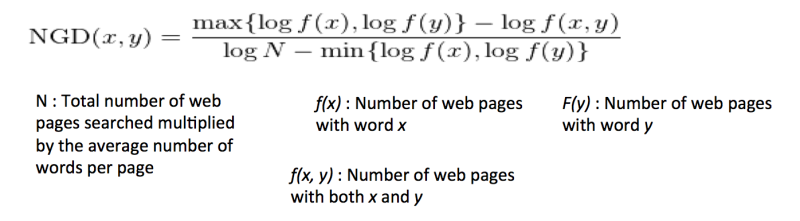
\includegraphics[width=.95\linewidth]{Figures/ngd.png}
  \caption{Normalized Google Distance}
  \label{fig:ngd}
\end{figure}

The biggest issue with discussed method is necessity of using search engines APIs, which have limitations and effectively stop many researchers from outside affiliated R\&D departments from conducting experiments at scale.

\subsection{Explicit Semantic Analysis} Explicit Semantic Analysis (ESA) \cite{gabrilovich2009wikipedia} is a technique of representing text using Wikipedia knowledge base and vast amount of human labelled data and analysing co-occurrences of words in the text. 

Words in articles are associated with articles' concept using TF-IDF scoring, and in effect word can be represented as a vector of its associations to each concept. In result semantic relatedness between pair of words can be measured with cosine similarity and document can be represented as the centroid of the vectors representing its words. In table below \ref{tab:esa-apple} is presented ranked list of concepts associated with word "apple":

\begin{table}[th]
\centering
 \begin{tabular}{| l | l |}
\hline
concept vector & relevance \\ \hline
Apple Specialist & 0.5189224482 \\ \hline
Ron Johnson (businessman) & 0.5182648301 \\ \hline
Apple Extended Keyboard & 0.4947317243 \\ \hline
Apple River Canyon State Park & 0.458741188 \\ \hline
Baldwin (apple) & 0.4552417099 \\ \hline
Golden Apple Award (education) & 0.3789061904 \\ \hline
 \end{tabular}
\caption{ESA concept vectors for "apple"}
\label{tab:esa-apple}
\end{table}

What is more ESA allows to calculate similarities between two words, what is very reliable measure of semantic relatedness. It has proven to perform much better than previous approaches based mainly on links structure analysis like Wikpedia Link-Based Measure (WLM) \cite{witten2008effective}. Comparison of results achieved by both methods is illustrated in table below \ref{tab:esa-wlm} where it can be clearly seen that ESA outperforms WLM. 

Despite being promising and well documented, ESA will not be used in further part of thesis. Unfortunately it does not yield semantic relatedness for far too many important pairs of words. It should be prepared on bigger corpus and then preprocessed leaving more infrequent words (less aggressively). In current configuration preprocessing would take almost a month, what is not acceptable from thesis perspective. 

\begin{table}[th]
\centering
 \begin{tabular}{| l | l | l |}
 \hline
Dataset & ESA & WLM \\ \hline
Miller and Charles & 0.73 & 0.70 \\ \hline
Rubenstein and Goodenough & 0.82 & 0.64 \\ \hline
WordSimilarity-353 & 0.75 & 0.69  \\ \hline
 \end{tabular}
\caption{ESA and WLM performance on three different datasets}
\label{tab:esa-wlm}
\end{table}

\subsection{Word2vec} Word2vec is a method proposed by Google \cite{mikolov2013efficient} to represent words as continuous vectors basing on two models - continuous bag of words (CBOW) or skip-gram (SG) discussed in previous chapter Background. As result of processing massive data sets with neural network, it embeds valuable information about words context and their semantic meaning \cite{mikolov2013exploiting}, \cite{zou2013bilingual}. Word2vec has proven to calculate similarity between words accurately yielding promising results \cite{wolf2014joint}, showing that it can eliminate ambiguities when performing both, clustering and classification tasks. Examples of applying word2vec model produced as a result of processing huge corpora produce interesting relations like:

\begin{itemize}
\item A is to B as X to Y (provided A, B, X)
\begin{itemize}
\item China is to Taiwan as Russia to [Ukraine, Moscow, Armenia]
\item king is to queen as man to [woman, girl]
\item knee is to leg as elbow to [forearm, arm]
\end{itemize}
\item A - B = C (provided A, B)
\begin{itemize}
\item Iraq - Violence = Jordan
\item President - Power = Prime Minister
\item Library - Books = Hall
\end{itemize}
\item Closest word vectors to Sweden: Norway, Denmark, Finland
\end{itemize}

There are many pre-trained sets of vectors, among them the most famous is trained on Google News dataset (about 100 billion words, 300-dimensional vectors for 3 million words and phrases), which will be used in further part of thesis \url{https://code.google.com/archive/p/word2vec/}

\chapter{Reproducible research} Apart from academic importance of article content, whether it is entirely new breakthrough algorithm or just minor modification of state of the art methods, there are a few crucial aspects of conducting research which make it reproducible. John Hopkins University course on Coursera: \url{https://goo.gl/qKKh1e} tries to bring researchers attention to this subject. It is, to certain extent, understandable that researchers are reluctant to share all their expertise and knowledge with strangers, even if these strangers are fellow researchers, as they compete for grants and prestige. However it is not only about greater good of science or becoming famous in particular domain, as in fairness majority of articles is not created with intention to be major contribution to domain. 

Obligation of producing articles in timely manner is often problematic and influences quality of research. Not putting a lot of effort into article, which does not make author proud is justified, but short sighted from greater good perspective. Conducting reproducible research requires more effort and takes longer of course but thinking about research community as about group of people, theoretically working separately, but jointly trying to move science forward, brings attention to need to act more responsibly. Preparing framework for reproducible research is beneficial to whole community. 

Following sections contain description of what in author's opinion can be improved and especially why benefits are worth the effort. Possible solutions, and more importantly, guidance for implementation, is outlined below. Naturally as an example is used domain of documents clustering.

\section{Reasons} 

\subsection{Reproducibility, Credibility and Trustworthiness} Well known experts can be mistaken and less known scientists are hardly to be trusted. Peer review unfortunately might be superficial and there are known cases when well known professor jokingly published paper which was later accepted to serious conference. Focusing on anomalies is pointless as number of authors whose number of citations, value of i10-index or h-index shows credibility is very limited.

Because vast majority of scientists and students producing articles and thesis are hardly trusted, showing exact flow of thoughts and describing process of conducting experiments thoroughly is a key to trustworthiness. Being able to reproduce results is major benefit to whole community as otherwise time spent on writing article is wasted.

\subsection{Data-sets and evaluation measures} It happens that one algorithm is tested on ODP-239 and MORESQUE datasets with regard to ARI and \mathit{F-measure} when other on MORESQUE and AMBIENT with regard to Entropy, Purity and \mathit{F-measure}. Denoting evaluation of particular algorithm on particular dataset with regard to particular measure in cube in which on one axis are available datasets on which DC algorithms tend to be evaluated, on second are possible DC evaluation measures and on third are DC algorithms, even when limiting each dimension to reasonable bounds still creates sparse cube. 

It would not be a problem if cost of filling blanks would not increase significantly with time. Hyperlinks became obsolete, new trends appear and authors forget. Expanding any dimension (like adding new algorithm or creating new dataset) is associated with unavoidable cost but it can be limited thanks to providing open source documentation. 

\subsection{Enriching sources} DC algorithms using WSI often make use of external knowledge sources like Wikipedia or Open Directory Project. Appearance of new promising knowledge source like BabelNet brings hope for improvement of results after incorporating it into chosen algorithms and with no modular construction of code or its openness such change is non trivial, but should be.

\subsection{Performance Improvements} Some algorithms might heavily exploit memory while others processing capacity. In any case there are periodically released new generations of processors, RAM (DDR 2,3,4), drives (HHD, SSD) and tools to orchestrate fleets of machines etc. Their appearance might be game changer for some algorithms as they might benefit more than others, not to mention that optimizing software usage for purpose of clustering task itself is interesting domain.

\subsection{Education} Properly conducted research sets great example for students and gives valuable insight into process of creating articles, conducting experiments and teaches every single step of the way. End result from education perspective might often be the least interesting and writing down thoughts, dead ends and way of thinking gives far more insight than just final paper being end result of many worth describing endeavours.

\subsection{Time-saving} Lack of documentation and open discussion on forum together with forgetting about the research details as time goes by, makes it hard for researcher to recall specifics of article, not to mention implementation details. Author being asked by other researchers or students about his article is wasting time on redundant questions, which could have been easily answered by community. Alternatively, due to lack of time, the scientist rejects request for help. Person prompting for help waits for response often many days, and even if it is positive, the author still has to clarify unnecessarily things which could have been written down in the first place.

\section{Rules of reproducible research} Allegory of conducting research in certain domain to business venture helps to understand what needs to be done. Poorly cooperating departments and subsidiaries lead to malfunctioning organization. The better individual contributors share their knowledge the better functioning is organization. Legacy, undocumented code and leaving responsible for it to co-workers leads to problems, which can be avoided by collecting not only final result of work but also know-how and intermediary steps (code, comments, scripts and notes), the same situation appears in case of articles. 

Research and code is never really done polished enough - scientists hesitate to share it at all, as well as other mentioned materials with fellow researchers. Shifting mindset to thinking about all fellow researchers as coworkers is crucial. Then it is possible to go step further, and maximize collective intelligence of worldwide researches as a group \url{https://goo.gl/wRSldy}. Taking all of the above into consideration, recommended course of action for avoiding unnecessary problems is to apply rules below:

\subsection{Open source code}  It is core to trustworthiness and reliable research. Huge factor of Lingo's and KeySRC's success, and their widespread usage as reference when evaluating results, apart from being efficient, was open sourced code. Once researcher shared it a lot of things which were ommited in paper, silent assumptions and not noticed side effects have potential of being found by community. Article can not be tested, but published code potentially will be by many users, what is not only benefcial for them but also researcher, thanks to possible contributions. 

Additionally apart from core algorithm code, there are many dependecies to which only author has references or at least knowledge from where to obtain them. Providing them with version numbers helps others to use the same setting and more inmportantly gathering datasets for evaluation, libraries for coding etc. is far easier and otherwise impossible to achieve unification is granted. Recommended platform which allow not only hosting of projects but also dedicated to them websites is GitHub \url{https://github.com/} and alternatively Bitbucket and GitLab

\subsection{Document technicalities and usage instructions} Writing down not only what kind of machines were used to conduct experiments in terms of SDD / HDD / RAM size and CPU cores and speed etc., but also environment details and setup instructions is not less important than code. Helping to copy research environment is of lesser importance in face of fact that often it has huge influence on specifics of implementation. For example Python code can run faster with $ O(n^2) $ complexity than $ O(n\log{n}) $ complexity just because using functions and structures having more efficient C routines underneath on certain architectures and settings.

\subsection{Intermediate results} Not publishing intermediate results is to certain extent understandable, but also should be avoided due to possibility of being suspected of selecting samples and evaluation measures in a way, that inconvenient results were discarded and bias was introduced. Not to mention that intermediate results can be used for sake of investigation of other researchers reaching beyond expectations of author. 

If files are too large to share, reproduction steps are enough. Without any of these value of research in eyes of community is questionable. Not only results of experiment can have intermediate results but also preprocessed data in program from which a lot can be inferred about research and is often as easy as adding line to create csv file.

\subsection{Lessons learned} Businessman discussing internals of running company and failures on the way with lessons learned is far more interesting than just presenting end product of his work (with regard to benefit of listeners not sales profits). Articles have limited conclusions section and often encountered problems are not discussed, in spite of fact, that it is the most important information, that can be shared back with community. Formulating them and making public as attachment to article or research for instance on Github would be certainly beneficial and requires no more than 5 minutes of work.

\chapter{Research engineering} In order to follow reproducible research rules from previous chapter, in this section equipment used to conduct experiments as well as tools and technologies with their descriptions will be discussed. For more details and information Github repository is used to have all information in one widely accessible place, allowing other people to comment and contribute. Everything can be found under link: \url{https://github.com/AdrianSzymczak/clustering-research}

\section{Development environment setup} Development has been performed on Ubuntu 16.04 running on DELL Inspiron 15 5559 laptop with 2 core Intel Core i5 i5-6200U processor, 16GB RAM and 240GB SSD. For sake of testing quickly pieces of code, local quick experiments were conducted on machine with 32GB RAM, 8 cores Intel Core i7 and 240GB SSD.

\section{Experiment environment setup} Amazon Web Services were used to set up experiment environment, specifically 4 machines model r3.8xlarge with 32 vCPU, 244 GB of RAM and 2 x 320 GB SSD which costs about 2.66 dollars per hour, depending on region. Total funds spend to conduct experiments amounted to about 275 dollars. 

Major advantage over other providers is low price although initial configuration had to be performed manually - installation of newest Docker, Python 2.7 and 3.5, Java 8 (Open JDK), all necessary libraries etc. Other providers like for instance Cloudera or Digital Ocean have almost everything pre-installed on their machines but do not scale that well and Azure, Google Cloud and Heroku are more expensive for approximately similar machines (if available at all).

Greatest advantage of using one powerful machine over many commodity servers is having results in one place and conducting experiments quickly instead of gathering results what adds complexity and influences experiment flow.

\section{Docker} Docker is open-source project designed to make deployment, creation and running applications easier for both developers and system administrators thanks to containerization. \url{https://www.docker.com/what-docker} Containers enable wrapping up applications with OS level elements providing everything needed to running code everywhere - starting from run-time through system tools and finishing on necessary third party libraries. 

It is not as heavy as virtualization but, thanks to Linux internals not to be discussed here, it feels light and is comparably powerful. From average user perspective convenience and portability is major advantage as for instance everything used for conducting research and experiments will run in the same manner disregarding differences in environment or operating system. It also runs well on AWS. 

\section{Python} Python \url{https://www.python.org/about/} is programing language broadly adapted in academia as learning curve, debugging and development cycle is extremely fast. It is interpreted, object-oriented, high-level language which serves as main scripting or glue language to connect existing libraries and software components together. With large variety of modules and packages, it is a go to solution for conducting research because often newest developments and algorithms from top articles are implemented in it. 

What is important when looking for open source implementation of some code with hope to be able to reuse it one should pay attention that Python 3.x is not an upgrade of Python 2.x - it is another branch and backward incompatibility is introduced intentionally to enable usage of brand new set of features. Instructions how to install both versions of Python can be found easily on the Internet.

\section{Java} Java is number one programming language \url{http://www.tiobe.com/tiobe-index/}. It is object-oriented high level-language intended to follow "write once run everywhere" rule. Because of being ubiquitous and so popular a lot of libraries are written in Java or at least on JVM (Scala, Clojure and Groovy are also JVM languages trying to enable doing more by writing less, thanks to functional nature) and thus have potential to allow researches to focus on core, providing everything else and avoid reinventing a wheel. JVM (Java Virtual Machine) is an abstract machine executing ".class" files containing Java precompiled programs (byte-code). JVM with library classes creates JRE (Java Runtime Environment) which together with development tools constitutes JDK (Java Development Kit). These components have separate releases to different platforms like Oracle JDK or Open JDK (mainly licensing). 

Nowadays Java 8 is recommended release and thanks to forward compatibility of Java 7 and 6 there should be no problem with incorporating libraries written in them in Java 8 code. There are many tutorials instructing how to install Java and one should not have problems with finding suitable one.

\section{Storage} During experiments vast majority of processed data came in form of archives containing text files. Because their structure was very simple and could easily be loaded to memory, no relational database was used. Despite being without doubt beneficial from engineering standpoint, for ease of development persistence was assured by making dumps of objects located in RAM to plain text files. To better support CRUD operations and improve ease of use in various scenarios in larger-scale experiments, for future reference following solutions are to be considered:

\subsection{Redis} Redis \url{http://redis.io/} is robust in-memory although persistent on disk database. As many Python libraries used in the thesis operate exclusively in-memory, machines used in experiment have lots of RAM. Operations in-memory are much faster than disk-based but especially important usecase when performing experiments is avoiding recomputing everything when rerunning experiments and keeping order among structures in memory.

\subsection{MongoDB} MongoDB is used as NoSQL document-oriented database because of being required data storage by EasyEsa and general ease of use, fitting into usecase of storing documents quite well.

\section{Libraries and tools} Making use of libraries broadly used in research community minimizes risk of committing error in implementation and prevents reinventing a wheel, simultaneously covering majority of use cases with satisfactory time and space complexity. In thesis following ones were used:

\subsection{NLTK} Python library \url{http://www.nltk.org/} which provides intuitive interfaces to over 50 corpora and lexical resources (among them the most importantly WordNet \url{https://wordnet.princeton.edu/}) which together with advanced text processing libraries for tokenization, stemming, classification, POS-tagging, filtering, parsing, semantic reasoning, wrappers etc. compose leading NLP library.

In thesis is used for text preprocessing according to algorithm description from next chapter.

\subsection{GENISM} Python library \url{https://radimrehurek.com/gensim/} for topic modelling and similarity retrieval with large text collections \cite{rehurek_lrec}. Among many other things GENSIM has efficient implementations of doc2vec, word2vec, TF-IDF, LDA, LDI, often calculated in distributed manner, and many more algorithms and methods of multilabel classification, dimensionality reduction, etc. \url{https://radimrehurek.com/gensim/apiref.html}. It is gaining momentum in NLP and IR community, thanks to being hassle-free and robust. It depends on other useful libraries like SciPy and NumPy which without going into details support scientific calculations in Python. 

In thesis is mainly used for handling word2vec and calculating semantic relatedness of words by calculating cosine distance between word2vec vectors.

\subsection{Scikit-learn} Python library \url{http://scikit-learn.org/} for data processing and analysis which implements great deal of algorithms and methods of classification, regression, clustering dimensionality reduction, model processing and preprocessingm and various evaluation methods. Similary to GENISM it depends on SciPy and NumPy, but additionally also on matplotlib. 
In thesis in mainly used for calculating evaluation metrics of clustering solutions.

\subsection{Pandas} Python library \url{http://pandas.pydata.org/} for data manipulation and analysis. It enables data structures and operations for manipulating numerical tables and time series. Thanks to fast and expressive data structures, working with relational and labeled data like in thesis both easy and intuitive.

In thesis served as tabular, in memory data storage for experiments results due to need for fast use of large variety of aggregating and indexing functions.

\subsection{EasyEsa} Described in details at \cite{carvalho2014easyesa} EasyESA, available under \url{http://treo.deri.ie/easyesa/}, is Java implementation of Explicit Semantic Analysis (ESA) which runs as a JSON webservice. It can be queried for the semantic relatedness measure between words and ranked list of concept vectors for given word. It is easy to use and has clear setup, usage instructions and provides scripts for preprocessing Wikipedia dump files, among other things.

In thesis was intended to be used to calculate semantic relatedness, but unfortunately too many pairs of words were not present to be successfully applied.

\section{IDEs} For both Python and Java popular environments are Vim, Emacs, Atom, Eclipse and Netbeans. Usually using one is absolutely personal choice although if someone has not tried it before, interesting IDE for Python is PyCharm and for Java IntelliJ, both described and available at \url{https://www.jetbrains.com}

\section{Other} Usage of RShiny studio \url{http://shiny.rstudio.com/} to visualize results of experiments is worth consideration. Moreover integration of clustering algorithm with Elasticsearch \url{https://www.elastic.co/} would allow it to be applied in large range of business scenarios. Linux software utilities for running processes and scheduling tasks are very useful, especially when conducting experiments on remote machines \url{https://en.wikipedia.org/wiki/Cron} 

\chapter{Novel algorithm} This chapter will focus on discussing novel document clustering algorithm, being major original contribution, using external knowledge sources for semantic relatedness (word2vec with SG model) and advanced NLP techniques. Step by step walk-trough and explanation together with pseudocode will be presented in details on example in following sections below. 

\vspace{1cm}
\begin{algorithmic}

\Function{Preprocess}{$text$}

    \State{MergeTitleTextFilterURL($text$)} 
    
	\State{Tokenize($text$)} 
	
	\State{PartOfSpeechTagging($text$)}
	
    \State{FilterPartsOfSpeech($text$)} 
	
	\State{RemoveStopWords($text$)} 
	
	\State{Lemmatize($text$)}	
	
	\State{Normalize($text$)} 
	
	\State{ExpandTuple($text$)} 
	
	\State \Return $text$
	
\EndFunction

\State{}

\Function{Fit}{$Query_i$, $DocSet$, $T_{semantic}$, $T_{node}$, $T_{edge}$, ${M}$}

    \State {$G \gets emptyGraph$}

    \State {$WordSimDict \gets emptySet$}
    
    \State {$AllQueryWords \gets emptySet$}
    
    \For{$Doc_i \in DocSet$} 

        \State{$WordsSet \gets $Set(Preprocess($Doc$))}
        
        \For{$k=0; k\le WordsSet.size; k++$} 
            
            \State {AddToSet($AllQueryWords, WordsSet[k])$}
        
            \For{$j=k+1; j\le WordsSet.size; j++$}

                \If {$WordsSet[k] \notin Query_i \land WordsSet[j] \notin Query_i$}
                
                    \State {AddToGraphOrUpdate$(G, WordsSet[(k, j)], inc=True$)}
                
                \EndIf
                
            \EndFor
            
        \EndFor
        
    \EndFor


    \For{$k=0; k\le AllQueryWords.size; k++$} 
    
        \For{$j=k+1; j\le AllQueryWords.size; j++$}

            \State {$maxSim \gets $ MaximumSimilarity$(AllQueryWords[k], AllQueryWords[j])$}
            
            \State {AddToDictionary$($WordSimDict$, (AllQueryWords[(k, j)])$}        
        
            \If {$AllQueryWords[k] \notin Query_i \land AllQueryWords[j] \notin Query_i$}
            
                \State {AddToGraphOrUpdate$(G, AllQueryWords[(k, j)],  maxSim$)}
            
            \EndIf
            
        \EndFor
        
    \EndFor

    \State {PruneGraph($G$, $T_{semantic}$, $T_{node}$, $T_{edge}$)}
    
    \State {$C \gets$ FindCliquesOrCommunities($G$, $M$)}
        
    \State \Return $WordSimDict$, $C$

\EndFunction

\State{}

\Function{Transform}{$DocSet$, $WordSimDict$, $C$, $T_{other}$, $T_{k}$}

    \State {$Matching \gets emptyMap$}
    
    \State {$DocumentsInCluster_{other} \gets emptySet $}
    
    \For{$C_i \in C$}
    
        \State {$DocumentsInCluster_i \gets emptySet $}
        
    \EndFor
    
    \For{$Doc_i \in DocSet$}
        
        \State {$C_{max} \gets null$}
    
        \For{$C_i \in C$}
        
            \If {Similarity($Doc_i$, $C_i$, $T_{k}$) \textgreater Similarity($Doc_i$, $C_{max}$, $T_{k}$)}
            
                \State {$C_{max} \gets C_i$}
                
            \EndIf
            
        \EndFor
        
        \If {Similarity($Doc_i$, $C_{max}) \ge T_{other}$}
           
            \State {AssignToCluster($DocumentsInCluster_{argmax}$, $Doc_i$)}
            
        \Else {\State {AssignToCluster($DocumentsInCluster_{other}$, $Doc_i$)}}
               
        \EndIf
        
    \EndFor
    
    \For{$C_i \in C$}
    
        \State {AddToMatching($Matching$, $C_i$, $DocumentsInCluster_i$)}
        
    \EndFor    
    
    \State {AddToMatching($Matching$, $C_{other}$, $DocumentsInCluster_{other}$)}

	\State \Return $Matching$
	
\EndFunction

\end{algorithmic}

\section{Preprocess} Preprocessing has to be done thoughtfully to avoid well known issue "gargabe in, garbage out". Because semantic relatedness between two single words is crucial for algorithm using cosine measure between word2vec vectors, the way how the data was preprocessed when vectors were created had to be taken into consideration. In the thesis set of vectors pre-trained on Google News (\url{https://code.google.com/archive/p/word2vec/} containting about 100 billion words, 300-dimensional vectors for 3 million words and phrases) is used. Because exact preprocessing steps were not clearly stated by Google, method producing corresponding results was proposed after analysis of provided corpus. Every single document is processed using NLP techniques in following manner:

\begin{enumerate}
\item MergeTitleTextFilterURL - title and snippet's text are joined together, URL is filtered out.
\item Tokenize - document is transformed to bag of words with split on whitespace.
\item PartOfSpeechTagging - POS tagging is performed for two reasons. Firstly to allow proper lemmatization (step 6) and secondly to enable filtering BOW (step 4).
\item FilterPartsOfSpeech - filtering based on POS tags, in effect of which only remaining tokens are these tagged as: adjectives, adverbs, verbs and nouns. What is important entity names and unclassified parts of speech, because of being possibly important, are treated as nouns and in effect are not filtered out.
\item RemoveStopWords - self explanatory.
\item Lemmatize - self explanatory.
\item Normalize - punctuation signs, single letters and numbers filtered out.
\item ExpandTuple - each word is expanded to tuple of 4 words consisting of:
\begin{itemize}
\item not lemmatized lowercase word
\item lemmatized lowercase word
\item not lemmatized word with letter case as in original word
\item original word
\end{itemize}
Explanation of logic standing behind this approach will be done on occasion of discussing graph construction in next section.
\end{enumerate}

Majority of methods above were implemented with use of previously discussed Python library NLTK \url{http://www.nltk.org/}. Exact implementation details are out of scope of thesis.

A set of documents with first column representing clusters (letter denotes one), second representing title, and third -- snippet is presented below. URL address is irrelevant from algorithm's perspective:

\begin{table}[th]
\centering
 \begin{tabular}{| c | p{3cm} | p{10cm} |}
 \hline
 1A &  Endangered animals &  Among many endangered species, mainly due to extensive hunting are... rhinos are in high demand because of horns \textbackslash\&amp rhino.png... their survival is questionable because eating meat requires hunting which is far more harder to catch than African grass.  \\ \hline
 1B &  Can tiger eat a lion? &  Why lion and tiger can be seen together only in a ZOO? 'cause in natural habitat these cats live in Asia or Africa! All animals who live usually in open air and run a lot suffer enormously while being held in cages - it's against their nature. \\ \hline
 1C &  Nature: Biology today &  so called "big cats" are properly called (following animal typology) members of "catine" familiy. They hunt down old or newborn zebras and antelopes and eat them without remorse. \\ \hline
 2A &  Icons of golf - history &  Tiger Woods A.K.A the best professional golf player ever... started training at the age of 2 what is early even as for world champion. Usually they don't start all day drills and practice (in local club or little league) before age of 6... He won first tournament in this noble disciplite at the age of 6 \\ \hline
 2B &  videos sport golf &  watch YouTube video "10 best shots"... with clubs that expensive you could also do it! of course after hard training... playing and practice will make you pro golf player but mind that trainer is a must in this demanding discipline - self coaching is not a way to win contests nowadays and became champion... diet, recovery, often supplements are necessary \\ \hline
 3C &  Best broadway shows &  Lion King was the best performance on broadway...  Disney made awesome job and Sir Elton John's music is outstanding. \\ \hline
\end{tabular}
\caption{Example search results}
\label{tab:searchresults}
\end{table}

After applying search results preprocessing strategy result illustrated in table \ref{tab:processedsearchresults} is obtained. These bag of words are used as input for further steps. The actual bag of words is a bag of tuples with words in original. lemmatized and lowercased variants - hence the calculation of maximum similarity between such two bag of tuples; from such tuple only the lemmatized lower case word is added as graph node.

This peculiar transformation is done due to dissonance arising from fact, that snippets are very short and for statistical significance of tokens the should be lowercased and lemmatized, but on the other hand word from word2vec model are unprocessed. In result word2vec words are case sensitive and appear both in lemmatized and not lemmatized form and yield significantly different results for similarity measure between two words in each of 16 possible variants. Analysis of distribution of similarities between various vectors joined with lack of information about words occurences or cooccurrences in Google News corpus and especially snippets length, resulted in applying straightforward solution of taking maximum similarity measure of total 16 was applied. It is not especially important 

\begin{table}[th]
\centering
 \begin{tabular}{| c | p{13cm} |}
 \hline
 1A &  endangered, animal, many, endanger, specie, mainly, due, extensive, hunting, rhino, high, demand, horn, amp, rhino.png, survival, questionable, eat, meat, require, hunt, far, hard, catch, african, grass \\ \hline
 1B &  tiger, eat, lion, lion, tiger, see, together, zoo, natural, habitat, cat, live, asia, africa, animal, live, usually, open, air, run, lot, suffer, enormously, hold, cage, 's, nature \\ \hline
 1C &  nature, biology, today, call, big, cat, properly, call, follow, animal, typology, member, catine, familiy, hunt, old, newborn, zebra, antelope, eat, remorse \\ \hline
 2A &  icons, golf, history, tiger, woods, a.k.a, best, professional, golf, player, ever, start, training, age, early, even, world, champion, usually, n't, start, day, drill, practice, local, club, little, league, age, first, tournament, noble, disciplite, age \\ \hline
 2B &  video, sport, golf, watch, youtube, video, best, shot, club, expensive, also, course, hard, training, playing, practice, make, pro, golf, player, mind, trainer, demanding, discipline, self, coaching, way, win, contest, nowadays, become, champion, diet, recovery, often, supplement, necessary \\ \hline
 3C &  best, broadway, show, lion, king, best, performance, broadway, disney, make, awesome, job, sir, elton, john, music, outstanding \\ \hline
1E	&	lorem, ipsum, document, intention, introduce, noise\\ \hline
 \end{tabular}
\caption{Preprocessed search results}
\label{tab:processedsearchresults}
\end{table}

\section{Fit} Each query is treated separately. After preprocessing search results all bag of words are used to create graph which will be used for inducing cluster labels and matching documents to clusters. 

Every single word which occurred in collection creates a node in graph, except query words (naturally previously preprocessed in the same manner as search results to bag of words form). For words appearing multiple times in collection only one node is created.

Later for every pair of nodes in graph an edge with two weights is created. First weight is semantic relatedness between words, calculated as cosine similarity between word2vec vectors. Possible values range froam 0 to 1, but 0 is also assigned if no similarity was found, what means that word was not frequent enough in word2vec corpus and should not be subject of concern. Second weight is a number of documents in which given 2 words represented by nodes appeared together, ranging from 0 to total number of search results (bags of words).

Also nodes have weights indicating in how many documents certain word was present.

For calculating edge weights, AddToGraphOrUpdate function in pseudo-code is used. In first loop that the function is used in, the occurrence and cooccurrence related weights are created and updated. In second loop, for set of all words the semantic weights are caclulated and appropriate edges updated or added.

We would like for the graph to represent the meaningful relations between words, i.e. if two words are connected with edge, they share context. After creating the graph it is a clique, hence it is useless for process of cluster derivation - we need to remove some edges and nodes. We call such process graph pruning, and it is a parametrized process. If semantic relatedness is below semantic threshold parameter, node frequency is below node frequency threshold parameter or aggregated amount of cooccurrences in the same documents is below cooccurrence threshold parameter, edge or node is removed from the graph. Semantic relatedness influences how strong is connection in terms of linking the words which are semantically similar and hence, such pair of words can be seen as some partial understandable description of potential subtopic to user. Aggregated amount of occurrences and cooccurrences in the same documents is measure of divisive potential and reduces potential noise.

The description above is reflected in the alogrithm pseudo-code with following three thresholds:
\begin{itemize}
    \item $T_{semantic}$ -- the minimum semantic weight for edge to be retained
    \item $T_{node}$ -- the minium weight for node to be retained (documents it occurs in)
    \item $T_{edge}$ -- the minimum weight for edge to be retained (number of documents the pair of words appear in)
\end{itemize}

\begin{figure}[!ht]
  \centering
    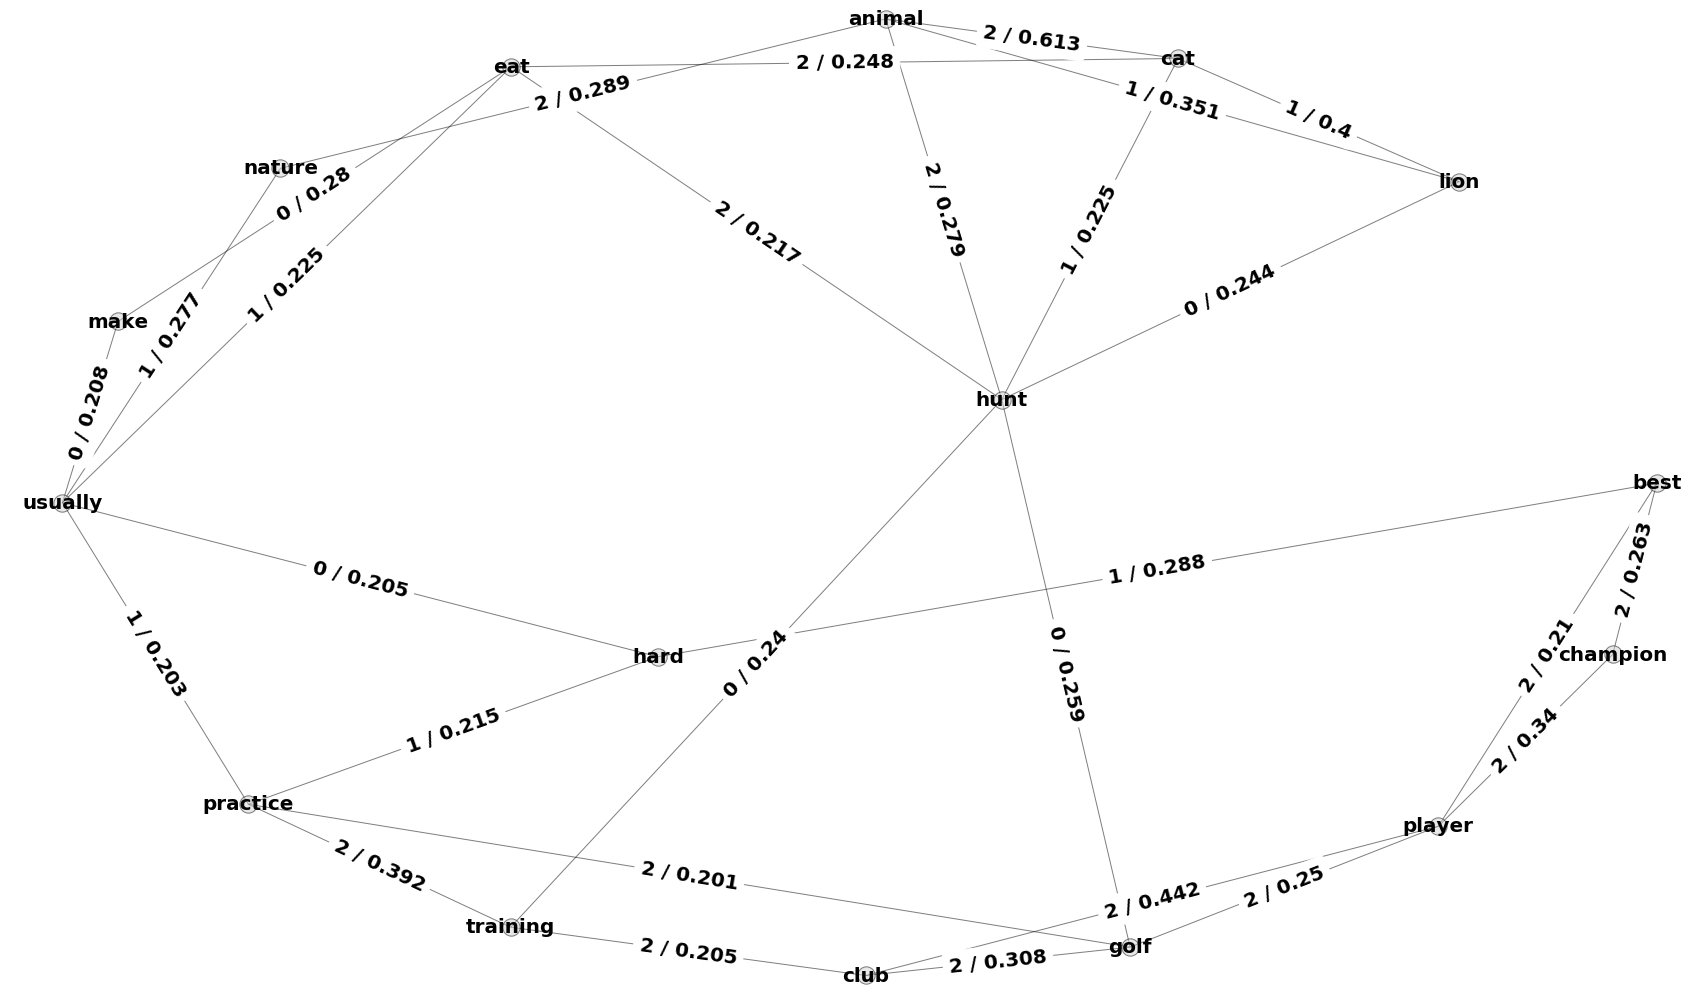
\includegraphics[width=1.0\textwidth]{final_graph_cropped}
    \caption{Pruned graph}
    \label{fig:prunedgraph}
\end{figure}

An example pruned graph created from documents set \ref{tab:searchresults} is presented on figure \ref{fig:prunedgraph}. The graph was created with use of following parameters:
\begin{itemize}
    \item $T_{semantic} = 0.2$
    \item $T_{node} = 2$
    \item $T_{edge} = 0$
    \item $M = 1$ (communities)
\end{itemize}

Having such pruned graph, the following step is to find the cliques in a graph. It is done for both values of parameter $M$ that stands for mode: cliques (0) and communities (1). For the cases where clique of size $k$ is part of clique of size $k+1$ only the latter will be included in the results. Nodes represented by words will be used directly as labels / keywords of created clusters. Making use of knowledge about human perception and how to optimize informativeness \cite{lidwell2010universal}, the most desired number of cluster labels is 3 or 4. However contrary to taking into account human perception, from the perspective of algorithm performance it may be better to have similar potential clusters merged together. Such process is called finding the communities in graph and is performed for parameter $M = 1$. It compares all the maximum cliques found in the graph, and merges the cliques of size $n$ if they share $n-1$ nodes.

\begin{table}[th]
\centering
 \begin{tabular}{| p{6cm} | c |}
 \hline
 best &  3 \\ \hline
 hard &  2 \\ \hline
 animal &  3 \\ \hline
 eat &  3 \\ \hline
 cat &  2 \\ \hline
 practice &  2 \\ \hline
 hunt &  2 \\ \hline
 lion &  2 \\ \hline
 club &  2 \\ \hline
 training &  2 \\ \hline
 make &  2 \\ \hline
 usually &  2 \\ \hline
 golf &  2 \\ \hline
 player &  2 \\ \hline
 nature &  2 \\ \hline
 champion &  2 \\ \hline
\end{tabular}
\caption{Example graph: node weights}
\label{tab:nodeweights}
\end{table}

\begin{table}[th]
\centering
 \begin{tabular}{| p{6cm} | p{6cm} | c | c |}
 \hline
 best &  hard &  1 &  0.29 \\ \hline
 best &  player &  2 &  0.21 \\ \hline
 best &  champion &  2 &  0.26 \\ \hline
 hard &  usually &  0 &  0.21 \\ \hline
 hard &  practice &  1 &  0.22 \\ \hline
 animal &  hunt &  2 &  0.28 \\ \hline
 animal &  cat &  2 &  0.61 \\ \hline
 animal &  lion &  1 &  0.35 \\ \hline
 animal &  nature &  2 &  0.29 \\ \hline
 eat &  cat &  2 &  0.25 \\ \hline
 eat &  usually &  1 &  0.22 \\ \hline
 eat &  hunt &  2 &  0.22 \\ \hline
 eat &  make &  0 &  0.28 \\ \hline
 cat &  hunt &  1 &  0.22 \\ \hline
 cat &  lion &  1 &  0.40 \\ \hline
 practice &  usually &  1 &  0.20 \\ \hline
 practice &  training &  2 &  0.39 \\ \hline
 practice &  golf &  2 &  0.20 \\ \hline
 hunt &  lion &  0 &  0.24 \\ \hline
 hunt &  training &  0 &  0.24 \\ \hline
 hunt &  golf &  0 &  0.26 \\ \hline
 club &  training &  2 &  0.20 \\ \hline
 club &  golf &  2 &  0.31 \\ \hline
 club &  player &  2 &  0.44 \\ \hline
 make &  usually &  0 &  0.21 \\ \hline
 usually &  nature &  1 &  0.28 \\ \hline
 golf &  player &  2 &  0.25 \\ \hline
 player &  champion &  2 &  0.34 \\ \hline
\end{tabular}
\caption{Example graph: edge weights and semantic weights}
\label{tab:edgeweights}
\end{table}

Potential clusters based on cliques from graph presented on figure \ref{fig:prunedgraph} are:
\begin{itemize}
    \item cat, eat, hunt
    \item animal, cat, hunt, lion
    \item eat, make, usually
    \item club, golf, player
    \item best, champion, player
    \item hard, practice, usually
\end{itemize}


Merging the cliques into communities results in following potential clusters:
\begin{itemize}
    \item club, golf, player
    \item eat, make, usually
    \item \textbf{best, champion, player}
    \item \textbf{animal, cat, eat, hunt, lion}
    \item hard, practice, usually    
\end{itemize}

The ones in bold were correctly matched for topics A and B, and for chosen parameters topic C was assigned to cluster "others".

\clearpage

\section{Transform} 

Having the potential clusters described by set of at least 3 words, the process of data transformation is to assign for each of the documents to one of the clusters.

Such process is done by comparing all the words from the document to all the words in potential cluster with use of word2vec similarity relatedness. For each word of the document, the best match for certain word in a given cluster is retained and then an average from a top $T_k$ number of document words (defined with parameter $T_k$) is calculated to determine the fit to a cluster. The document is then assigned to the cluster for which it has the highest average similarity if it exceeds the minimum assignment threshold $T_{other}$. For documents that do not exceed the threshold a common cluster for "other" documents is assigned.

In the presented example, the parameters were set as follows:
\begin{itemize}
    \item $T_{k} = 3$
    \item $T_{other} = 0.8$
\end{itemize}

And as mentioned in previous section, the cluster assignment corresponds to gold standard.

\chapter{Evaluation} Following chapter focuses on concluding thesis by discussing evaluation, experiment and its results as well as proposal of further work. Additionally performs assessment whether initial objectives were completed and original contributions were delivered.

\section{Experiment design}

The experiment was conducted for each possible variation of the following parameters values:

\begin{itemize}
    \item $M$: 0 (cliques), 1 (communities)
    \item $T_{node}$: 1, 2
    \item $T_{edge}$: 0, 1
    \item $T_{semantic}$: 0.25, 0.3, 0.35, 0.4, 0.45, 0.5, 0.55, 0.6, 0.65, 0.7, 0.75, 0.8
    \item $T_{k}$: 2, 3, 4, 5, 6, 7
    \item $T_{other}$: 0.0, 0.05, 0.1, 0.15, 0.2, 0.25, 0.3, 0.35, 0.4
\end{itemize}

Such variation allowed to analyse in detail the behaviour of proposed algorithm.

\section{Optimal results}\label{section:optimal}

For the case of results analysis we have focused on four measures:
\begin{itemize}
    \item Adjusted Mutual Information (AMI), see \ref{section:MutualInformation}
    \item Adjusted Rand Index (ARI), see \ref{section:RandIndex}
    \item \mathit{F-measure}, see \ref{section:FMeasure}
    \item Jaccard index, see \ref{section:Jaccard}
\end{itemize}

An attempt to implement the alternative version of \mathit{F-measure} was also made, however it was not straightforward what formulation, that cluster with other documents was ignored exactly meant. The recreated version of the measure yielded different results on baselines proposed in \cite{di2013clustering}, hence the measure is not used in comparison.

Each of mentioned measures was calculated at first at the query level. The documents were assigned to the cluster created by the algorithm or, in case where none of potential clusters were appropriate, to cluster with other documents. As the number of documents in each of the queries is in most cases exactly 100 and in some very close to 100, a classic average from all the queries was calculated for each of the datasets for each measure.

The table \ref{tab:optimal} presents the best results from the whole experiments for certain measure and dataset together with the results on all the measures and the parameters that were used in particular best case.

\begin{table}[th]
\centering
\begin{tabular}{ll|rrrr|rrr}
\toprule
  dataset &    measure &    \rotatebox{60}{AMI} &    \rotatebox{60}{ARI} &  \rotatebox{60}{\mathit{F-measure}} &  \rotatebox{60}{Jaccard} &  $T_{sem}$ &  $T_{other}$ &  $T_{k}$ \\
\midrule
  Ambient &        AMI & \textbf{0.1918} & 0.1575 &     0.3917 &   0.2498 & 0.25 &   0.40 &    7 \\
  Ambient &        ARI & 0.1918 & \textbf{0.1575} &     0.3917 &   0.2498 & 0.25 &   0.40 &    7 \\
  Ambient &  \mathit{F-measure} & 0.0064 & 0.0067 &     \textbf{0.5321} &   0.3719 & 0.70 &   0.40 &    3 \\
  Ambient &    Jaccard & 0.0064 & 0.0067 &     0.5321 &   \textbf{0.3719} & 0.70 &   0.40 &    3 \\ \hline
 Moresque &        AMI & \textbf{0.1247} & 0.1326 &     0.5089 &   0.3570 & 0.40 &   0.40 &    5 \\
 Moresque &        ARI & 0.1247 & \textbf{0.1326} &     0.5089 &   0.3570 & 0.40 &   0.40 &    5 \\
 Moresque &  \mathit{F-measure} & 0.0001 & 0.0003 &     \textbf{0.6703} &   0.5235 & 0.80 &   0.15 &    5 \\
 Moresque &    Jaccard & 0.0001 & 0.0003 &     0.6703 &   \textbf{0.5235} & 0.80 &   0.15 &    5 \\ \hline
   Odp239 &        AMI &\textbf{0.1730}  & 0.1322 &     0.3046 &   0.1851 & 0.40 &   0.40 &    2 \\
   Odp239 &        ARI & 0.1700 & \textbf{0.1357} &     0.3219 &   0.1992 & 0.40 &   0.35 &    4 \\
   Odp239 &  \mathit{F-measure} & 0.0735 & 0.0710 &     \textbf{0.3647} &   0.2312 & 0.55 &   0.40 &    2 \\
   Odp239 &    Jaccard & 0.0690 & 0.0678 &     0.3645 &   \textbf{0.2313} & 0.55 &   0.35 &    2 \\
\bottomrule
\end{tabular}
\caption{Optimal results from the whole experiments per dataset and measure, for all cases $M = 1 (communities), T_{node} = 2, T_{edge} = 1$}
\label{tab:optimal}
\end{table}

\clearpage

\section{Parameter values study}

In section \ref{section:optimal} we have seen what were the best parameters taking into account certain measures only. From practical usage point of view, such approach is of course not adequate. In this section we will analyse, using the top-down approach, influence of various parameters on certain measures for certain datasets.

For the anlaysis of the parameter influence we would like to exclude all the results that would be rejected should the algorithm was implemented in some production system. Hence we do not include in any calculations in this chapter the results that were not yielding an assignment to at least 3 clusters.

\subsection{First level parameters}

At first we will try to find the best combination of parameters:
\begin{itemize}
    \item $M$
    \item $T_{node}$
    \item $T_{edge}$
\end{itemize}

As in our experiment each of the parameters has possible two values, it gives us 8 combinations. As we want to analyse influence of these parameters only, regardless of the rest -- we need to aggregate the results in proper manner.

There are some variations of parameters that are extremely unoptimal, yeilding inappropriate results. In order to avoid such extremes, for each combination of $M$, $T_{node}$, $T_{edge}$ we calculate the median of results for certain measure on query level. Then we calculate the average from queries on dataset level (we do not take median, as in case of queries it is desirable to include any potential extreme results if such are present).

We present the results in tables \ref{tab:initparamstablep1} and \ref{tab:initparamstablep2} as well as on figure \ref{fig:initparamsfig1} for Adjusted Mutual Information, \ref{fig:initparamsfig2} for Adjusted Rand Index, \ref{fig:initparamsfig3} for \mathit{F-measure} and \ref{fig:initparamsfig4} for Jaccard index.

\begin{figure}[h]
  \centering
  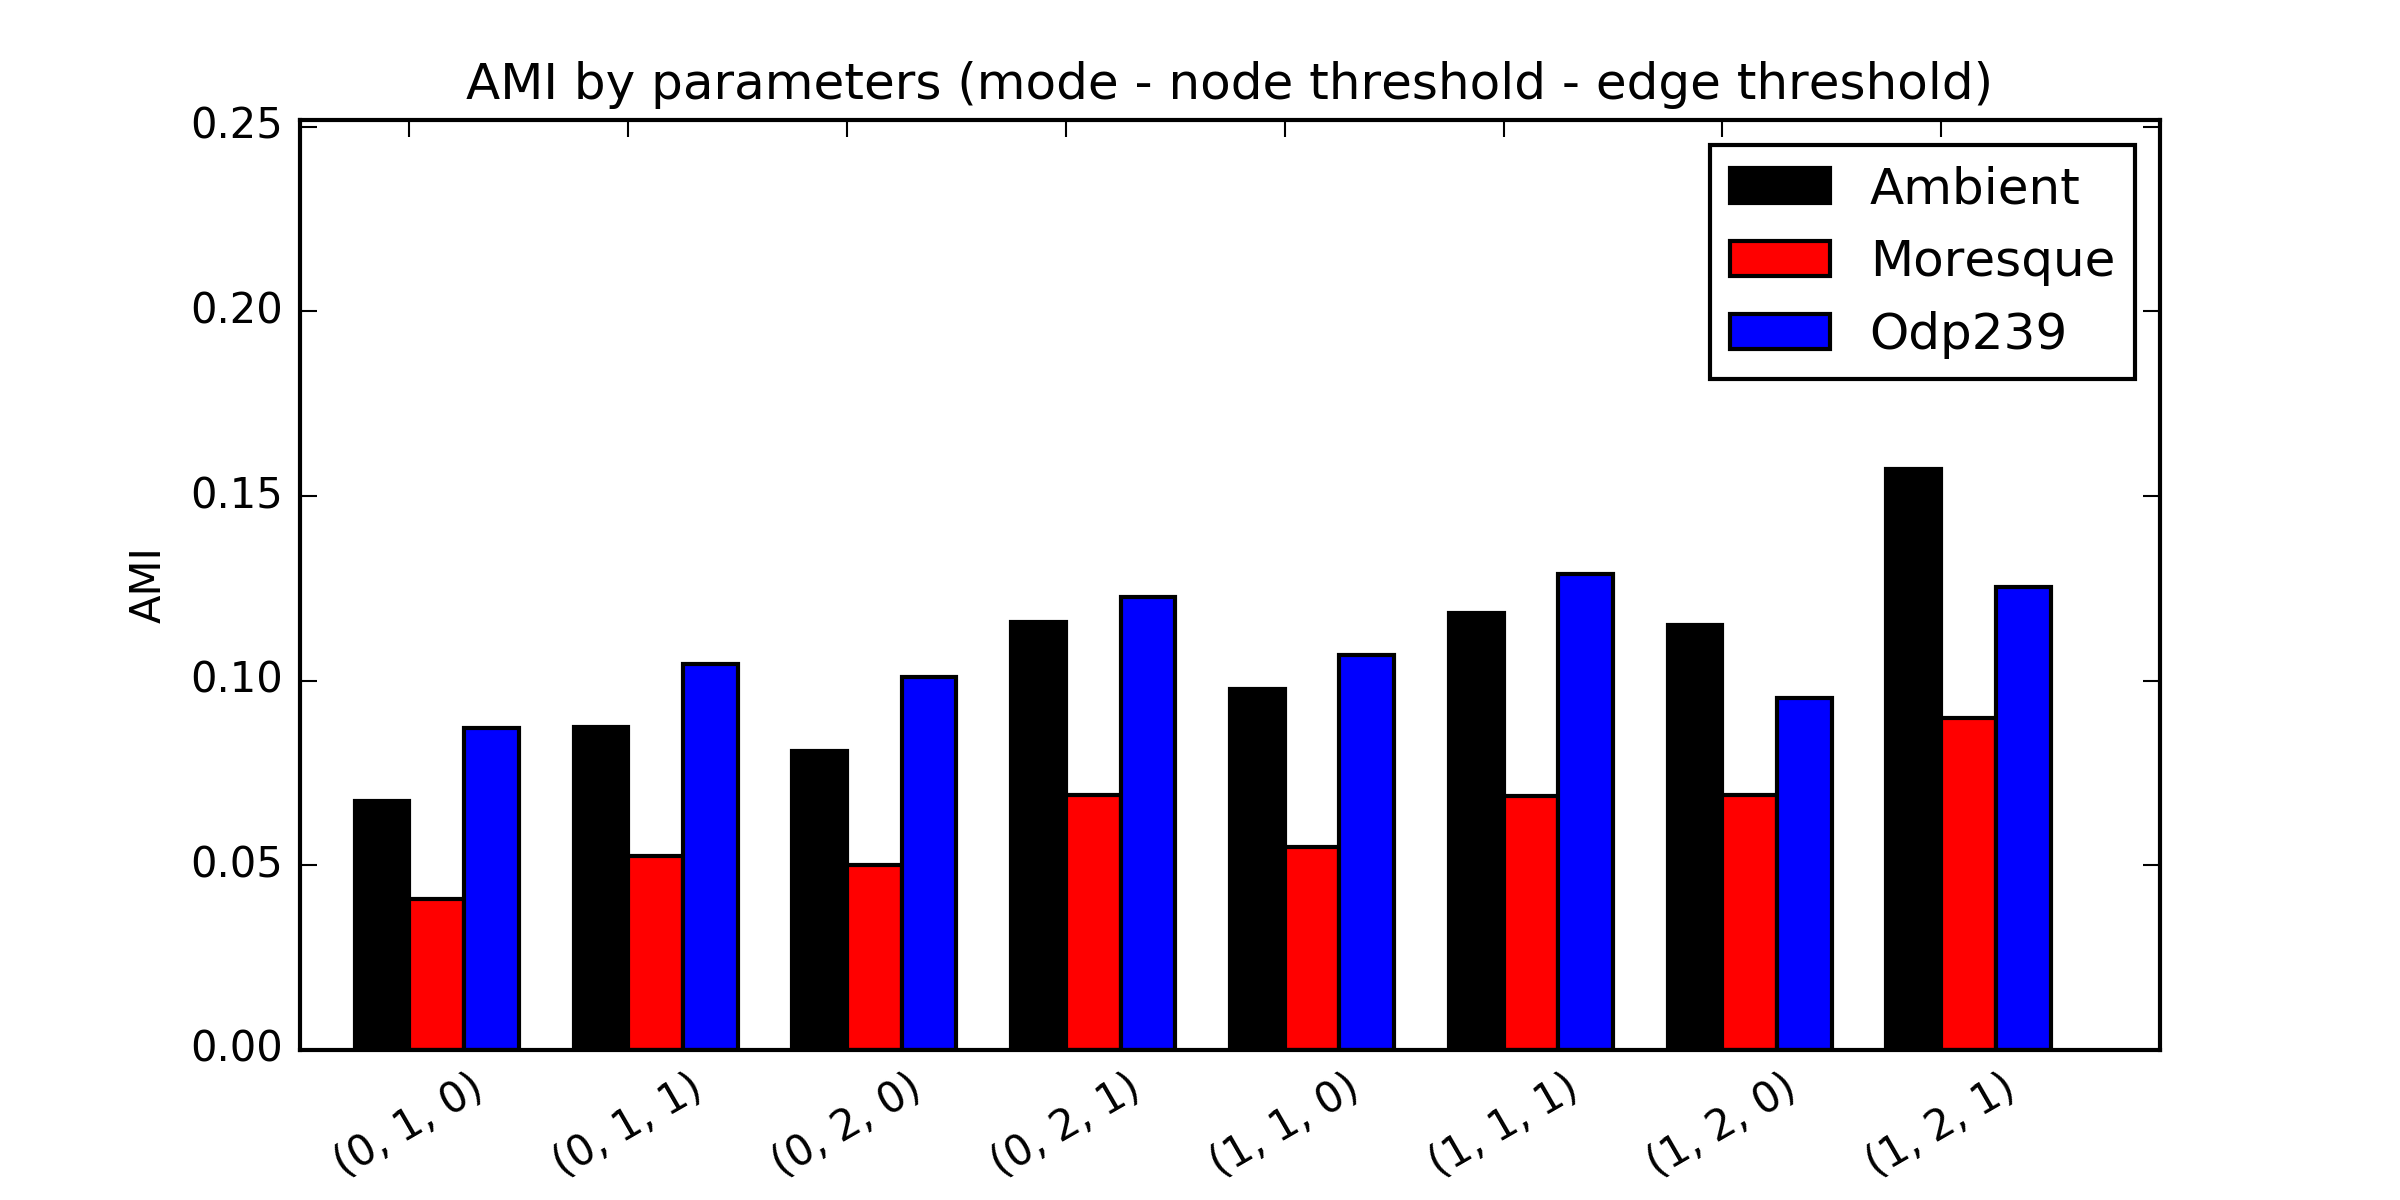
\includegraphics[width=1.0\linewidth]{Figures/initial_params_reult_AMI.png}
  \caption{Initial parameters results for Adjusted Mutual Information}
  \label{fig:initparamsfig1}
\end{figure}

\begin{figure}[h]
  \centering
  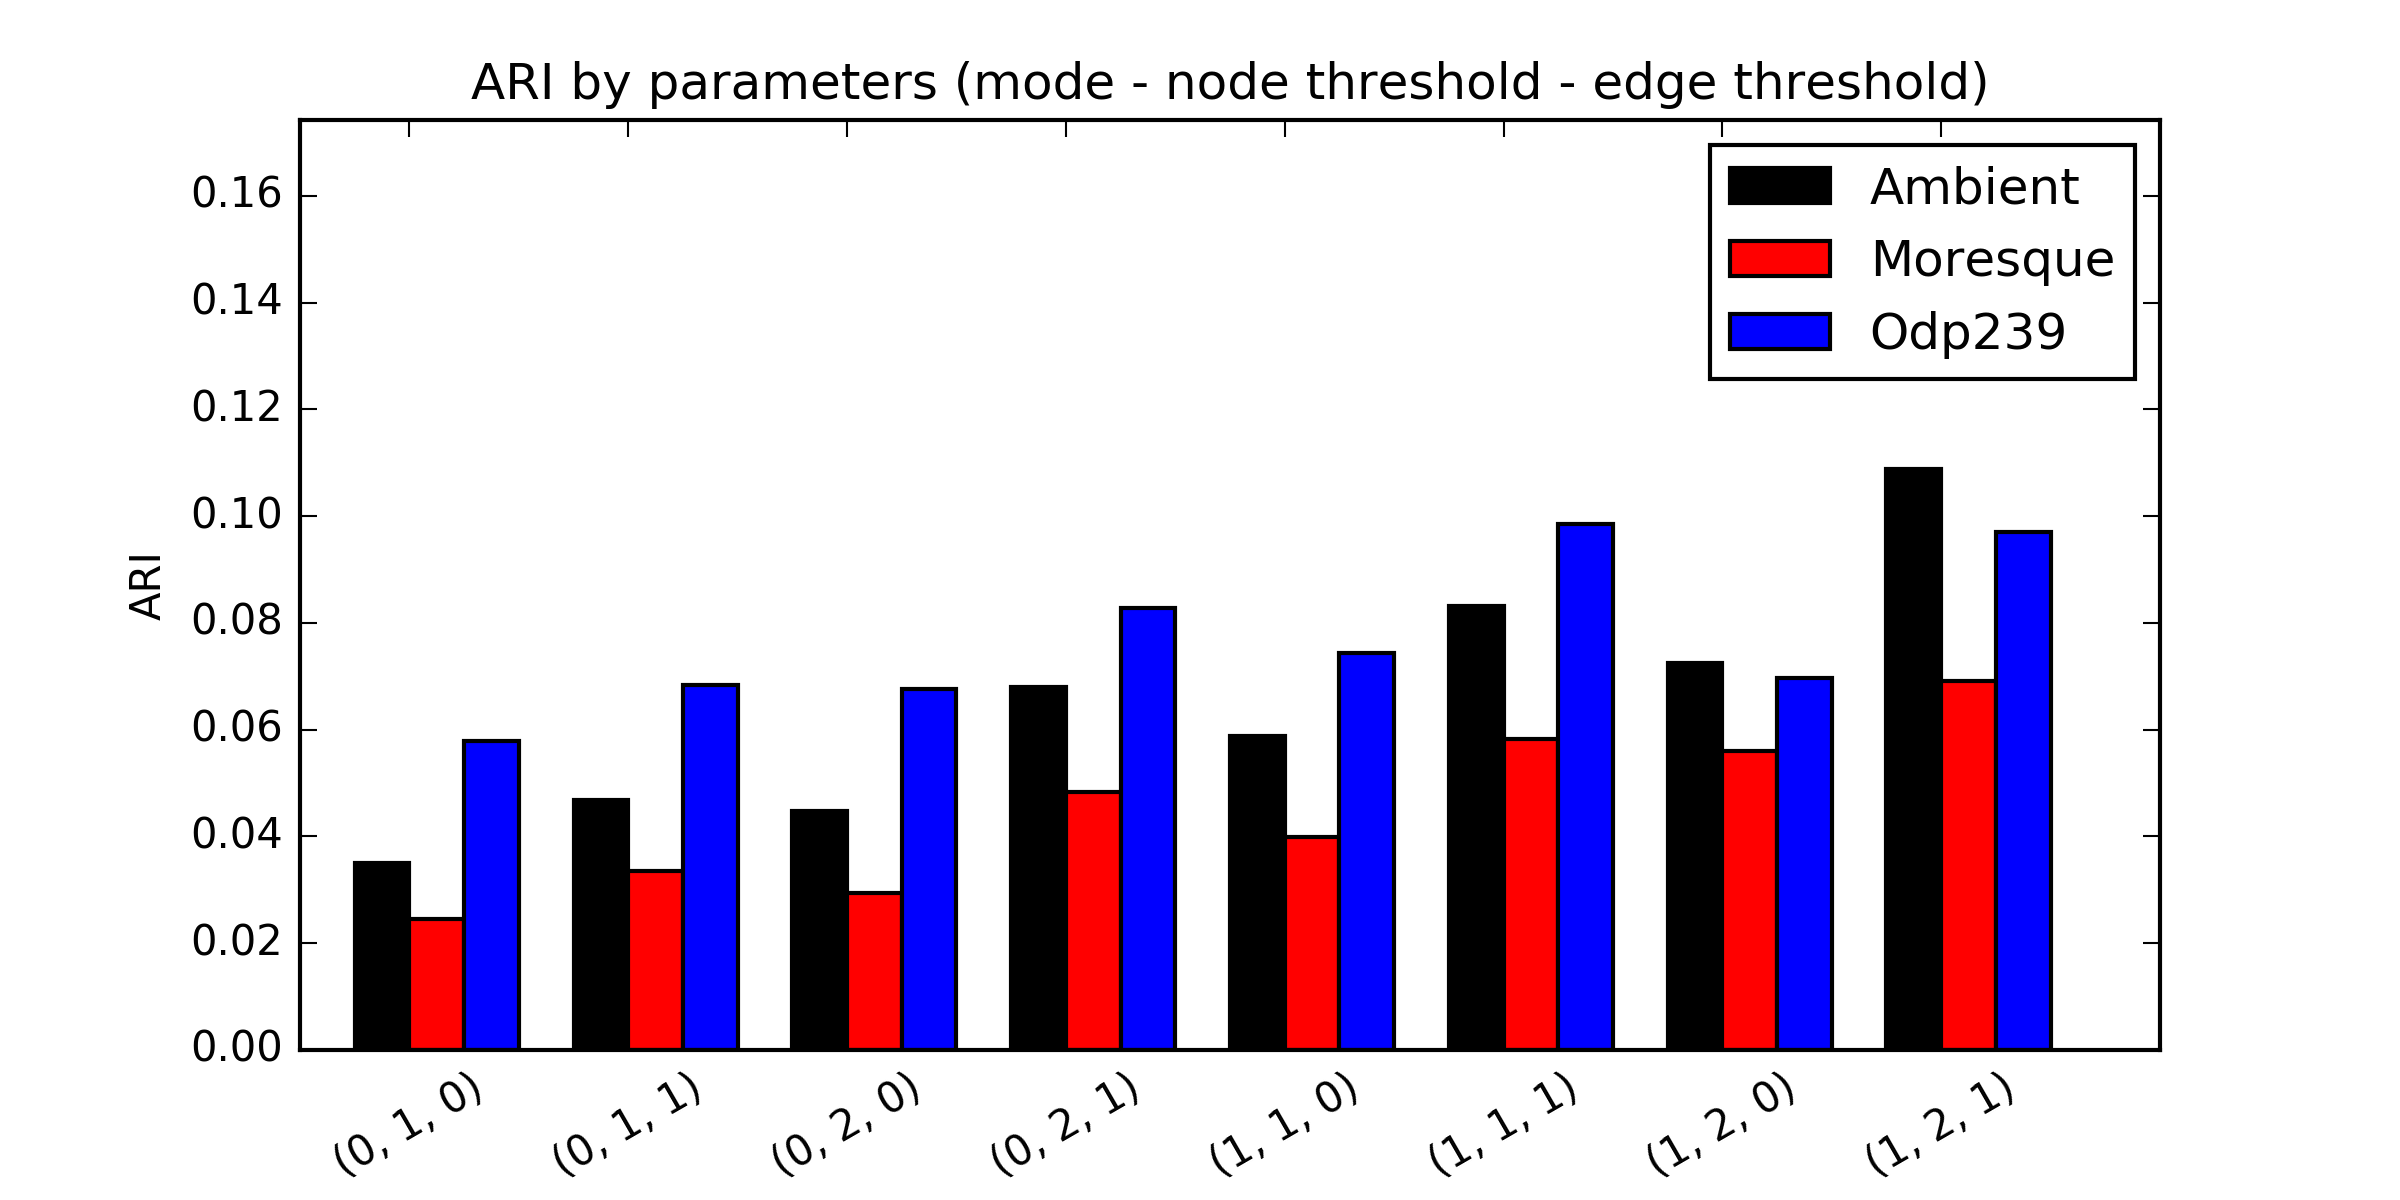
\includegraphics[width=1.0\linewidth]{Figures/initial_params_reult_ARI.png}
  \caption{Initial parameters results for Adjusted Rand Index}
  \label{fig:initparamsfig2}
\end{figure}

\begin{figure}[h]
  \centering
  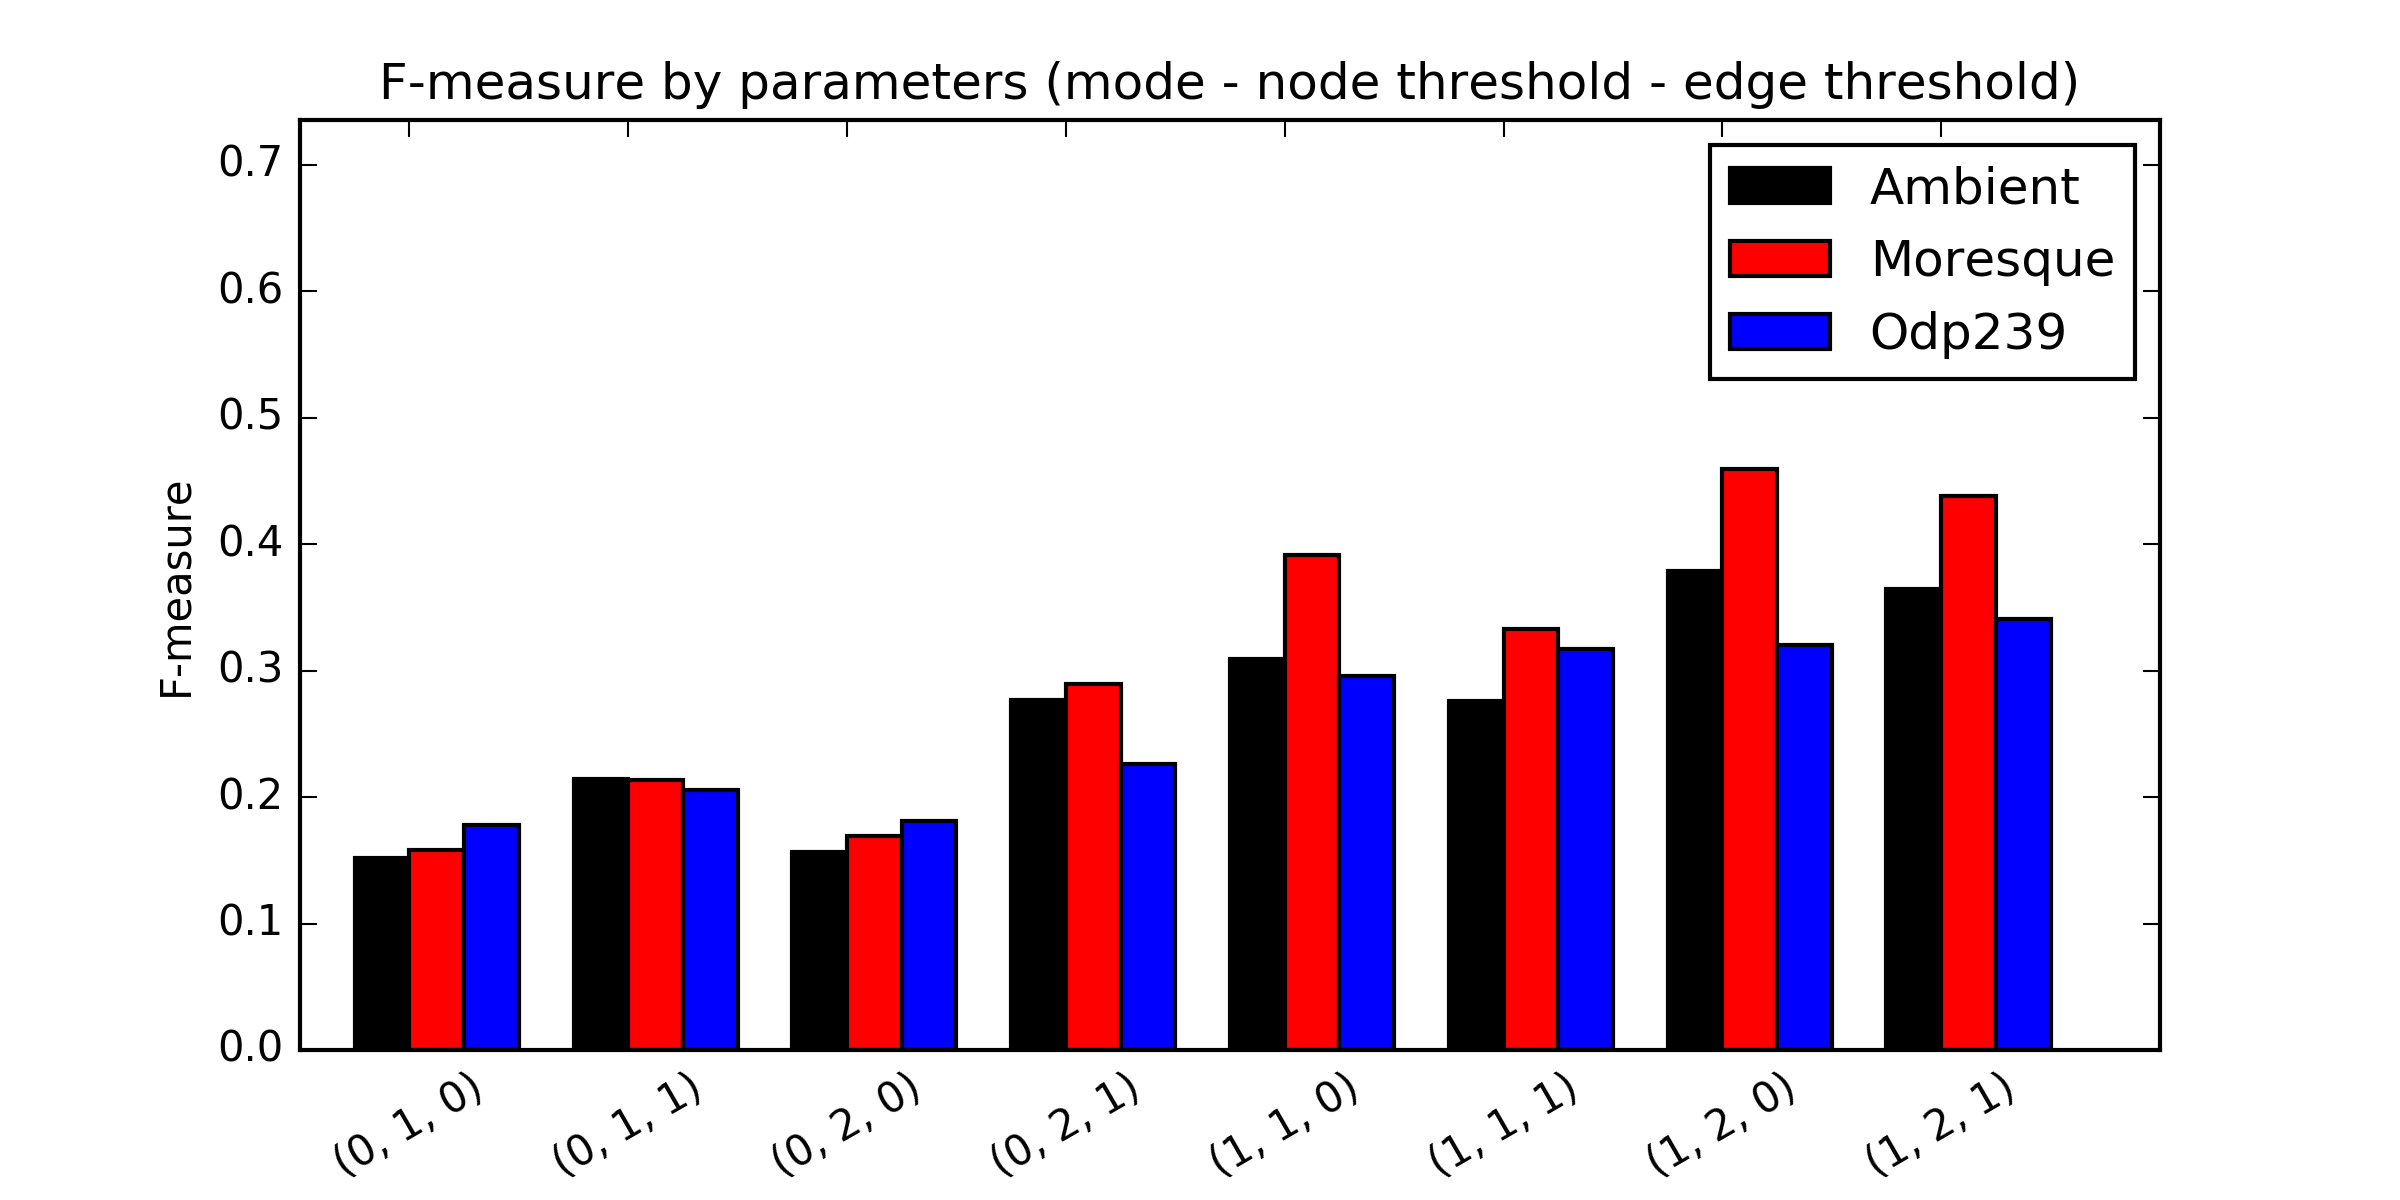
\includegraphics[width=1.0\linewidth]{Figures/initial_params_reult_F-measure-classic.png}
  \caption{Initial parameters results for \mathit{F-measure}}
  \label{fig:initparamsfig3}
\end{figure}

\begin{figure}[h]
  \centering
  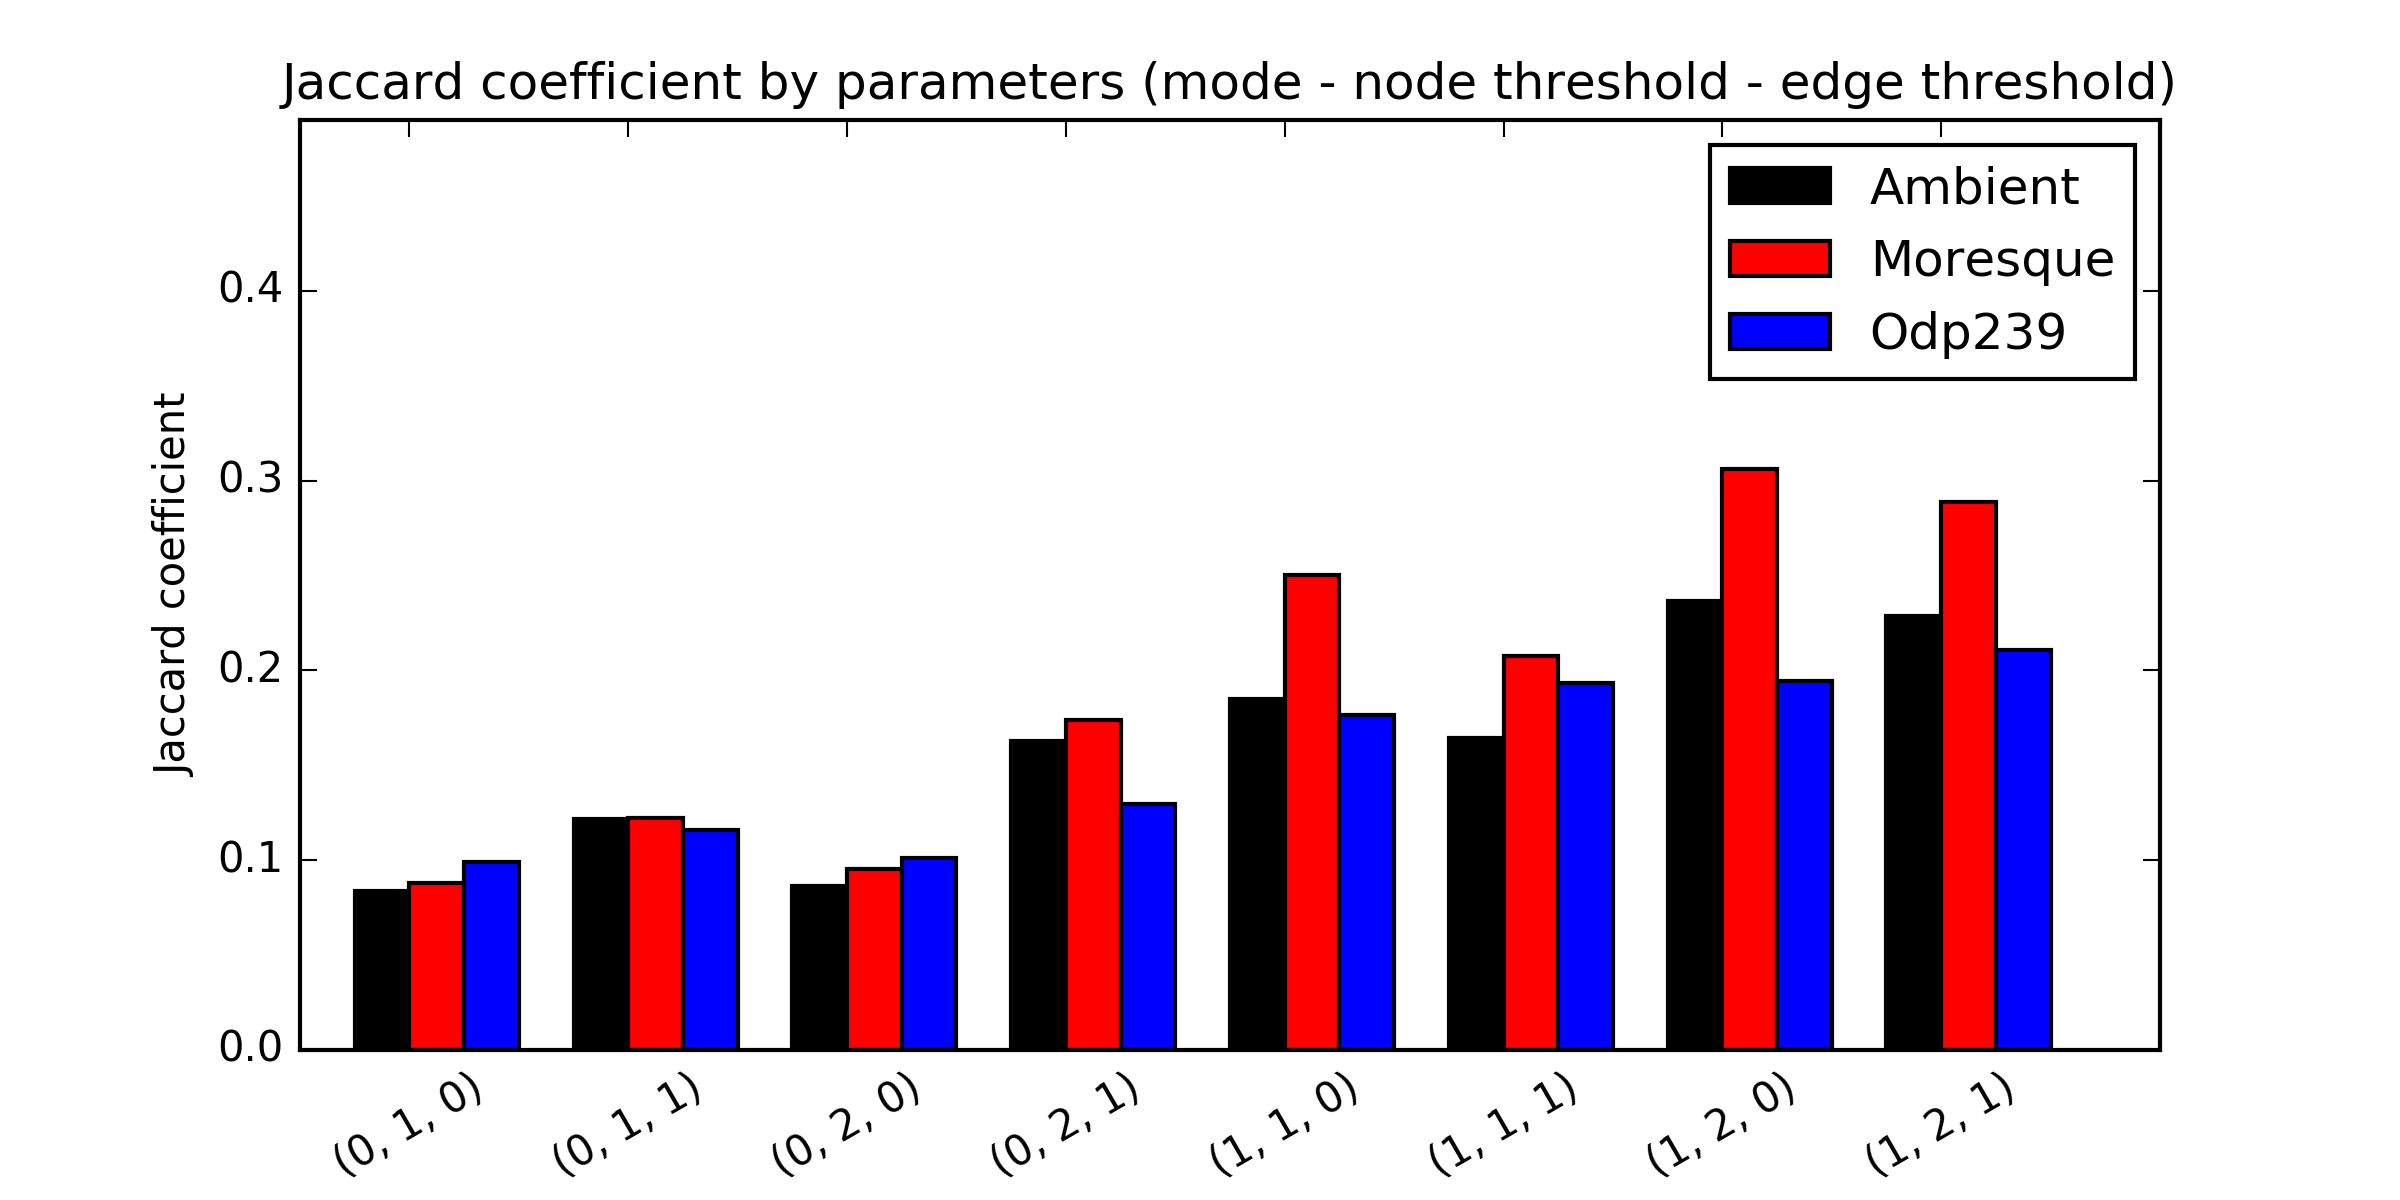
\includegraphics[width=1.0\linewidth]{Figures/initial_params_reult_Jaccard.png}
  \caption{Initial parameters results for Jaccard coefficient}
  \label{fig:initparamsfig4}
\end{figure}

\begin{table}[th]
\centering
\begin{tabular}{lll|rrr|rrr}
\toprule
  &   &   & Jaccard &          &        &     ARI &          &        \\
  &   &   & \rotatebox{60}{Ambient} & \rotatebox{60}{Moresque} & \rotatebox{60}{Odp239} &           \rotatebox{60}{Ambient} & \rotatebox{60}{Moresque} & \rotatebox{60}{Odp239} \\
$M$ & $T_{node}$ & $T_{edge}$ &         &          &        &         &          &        \\
\midrule
0 & 1 & 0 &    0.08 &     0.09 &   0.10 &    0.04 &     0.02 &   0.06 \\
  &   & 1 &    0.12 &     0.12 &   0.12 &    0.05 &     0.03 &   0.07 \\
  & 2 & 0 &    0.09 &     0.10 &   0.10 &    0.04 &     0.03 &   0.07 \\
  &   & 1 &    0.16 &     0.17 &   0.13 &    0.07 &     0.05 &   0.08 \\
1 & 1 & 0 &    0.19 &     0.25 &   0.18 &    0.06 &     0.04 &   0.07 \\
  &   & 1 &    0.16 &     0.21 &   0.19 &    0.08 &     0.06 &   0.10 \\
  & 2 & 0 &    0.24 &     0.31 &   0.19 &    0.07 &     0.06 &   0.07 \\
  &   & 1 &    0.23 &     0.29 &   0.21 &    0.11 &     0.07 &   0.10 \\
\bottomrule
\end{tabular}
\caption{Initial parameters results table: Jaccard and ARI}
\label{tab:initparamstablep1}
\end{table}

\begin{table}[th]
\centering
\begin{tabular}{lll|rrr|rrr}
\toprule
  &   &   &     AMI &          &        & \mathit{F-measure} &          &        \\
  &   &   & \rotatebox{60}{Ambient} & \rotatebox{60}{Moresque} & \rotatebox{60}{Odp239} &           \rotatebox{60}{Ambient} & \rotatebox{60}{Moresque} & \rotatebox{60}{Odp239} \\
$M$ & $T_{node}$ & $T_{edge}$ &         &          &        &                   &          &        \\
\midrule
0 & 1 & 0 &    0.07 &     0.04 &   0.09 &              0.15 &     0.16 &   0.18 \\
  &   & 1 &    0.09 &     0.05 &   0.10 &              0.21 &     0.21 &   0.21 \\
  & 2 & 0 &    0.08 &     0.05 &   0.10 &              0.16 &     0.17 &   0.18 \\
  &   & 1 &    0.12 &     0.07 &   0.12 &              0.28 &     0.29 &   0.23 \\
1 & 1 & 0 &    0.10 &     0.05 &   0.11 &              0.31 &     0.39 &   0.30 \\
  &   & 1 &    0.12 &     0.07 &   0.13 &              0.28 &     0.33 &   0.32 \\
  & 2 & 0 &    0.12 &     0.07 &   0.10 &              0.38 &     0.46 &   0.32 \\
  &   & 1 &    0.16 &     0.09 &   0.13 &              0.36 &     0.44 &   0.34 \\
\bottomrule
\end{tabular}
\caption{Initial parameters results table: AMI and \mathit{F-measure}}
\label{tab:initparamstablep2}
\end{table}

\clearpage

For further analysis of the parameters we would like to choose the best combination of analysed parameters. In order to do so we have ranked the results on each of measures from 1 to 8, calculated the sum of ranks for each combination and chosen the lowest one for each dataset. In each case the optimal combination was:
\begin{itemize}
    \item $M = 1$ (communities)
    \item $T_{node} = 2$
    \item $T_{edge} = 1$
\end{itemize}

Such parameters also have proven the optimal choice for the best results according to all the measures and for all the datasets (see table \ref{tab:optimal}).

\section{Second level parameters}

As a second level parameter we will analyse the semantic threshold value $T_{sem}$. 

Having the experiment results filtered to chosen parameters $M = 1$ (communities), $T_{node} = 2$ and $T_{edge} = 1$, and taking into account the fact, that we analyse only the results that assigned the documents to at least three clusters, let's take a look at the statistics of how many queries within certain dataset have at least one appropriate result for the analysis (table \ref{tab:fallback}).

\begin{table}[th]
\centering
\begin{tabular}{lrrr}
\toprule
{} &  Ambient &  Moresque &  Odp239 \\
T_{sem} &          &           &         \\
\midrule
0.25  &       44 &       114 &     239 \\
0.30  &       44 &       113 &     239 \\
0.35  &       44 &       112 &     237 \\
0.40  &       43 &       108 &     219 \\
0.45  &       37 &        92 &     187 \\
0.50  &       26 &        67 &     145 \\
0.55  &       14 &        33 &      84 \\
0.60  &        5 &        19 &      45 \\
0.65  &        3 &         9 &      16 \\
0.70  &        0 &         2 &       3 \\
0.75  &        0 &         0 &       1 \\
\bottomrule
\end{tabular}
\caption{Number of queries yielding at least 3 cluster assignments for given T_{sem}}
\label{tab:fallback}
\end{table}

In order to conduct a proper analysis we are introducing "fallback rule". So for queries, that do not have entry with certain value of $T_{sem}$ we take the largest possible value they had.

Another challenge is to abstract from the values of $T_k$ and $T_{other}$. Using the median in this case would be inappropriate especially for the relation between $T_{sem}$ and $T_{other}$, that are operating on the same measure and optimal $T_{other}$ would be expected to be different for different $T_{sem}$ values. Also the analysed datasets are specific, so various parameters are expected to work well for them. Taking into account these facts and inability to use median, for each group defined by:
\begin{itemize}
    \item dataset
    \item $T_{sem}$
    \item $T_k$
    \item $T_{other}$
\end{itemize}

we calculate average value of all the measures that we take into account. Then, we calculate the rank of pair $T_k$ and $T_{other}$ for each pair of dataset and $T_{sem}$ and for each measure. We finally create the final rank by adding the ranks for all the measures together. It results in fixed pair of $T_k$ and $T_{other}$ for each pair of dataset and $T_{sem}.

With all the prerequisits described in mind, the results of influence of $T_{sem}$ are presented on figures: \ref{fig:semparamfig1} for Adjustem Mutual Information, \ref{fig:semparamfig2} for Adjusted Rand Index, \ref{fig:semparamfig3} for \mathit{F-measure} and \ref{fig:semparamfig4} for Jaccard index as well as tables: \ref{tab:semparamtablep1} and \ref{tab:semparamtablep2}


\begin{figure}[h]
  \centering
  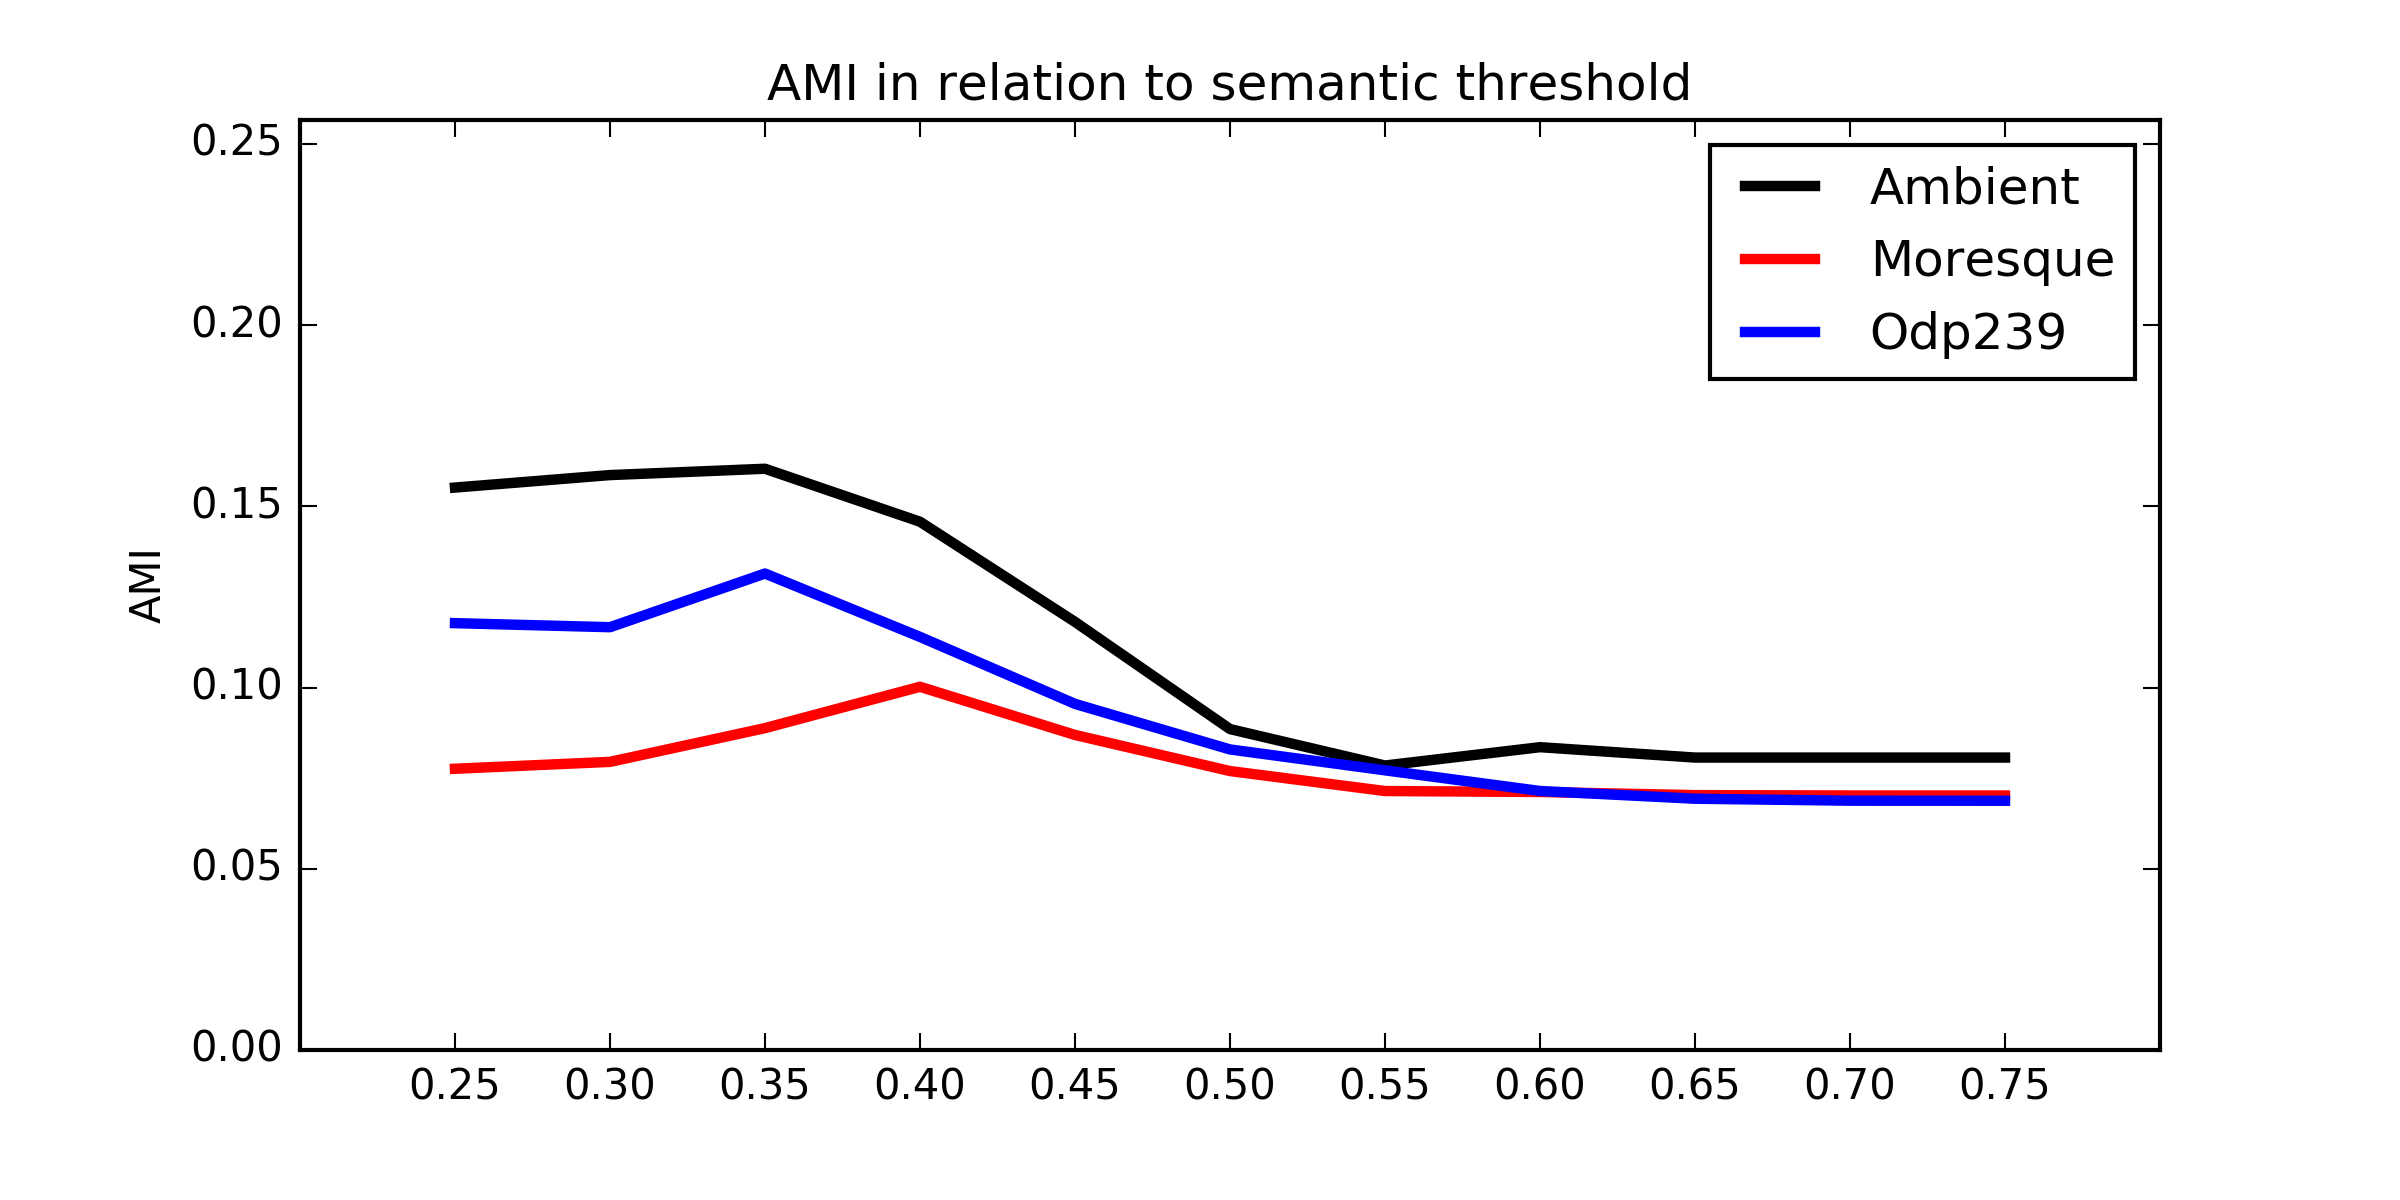
\includegraphics[width=1.0\linewidth]{Figures/sem_threshold_reult_AMI.png}
  \caption{Semantic threshold influence on Adjusted Mutual Information}
  \label{fig:semparamfig1}
\end{figure}

\begin{figure}[h]
  \centering
  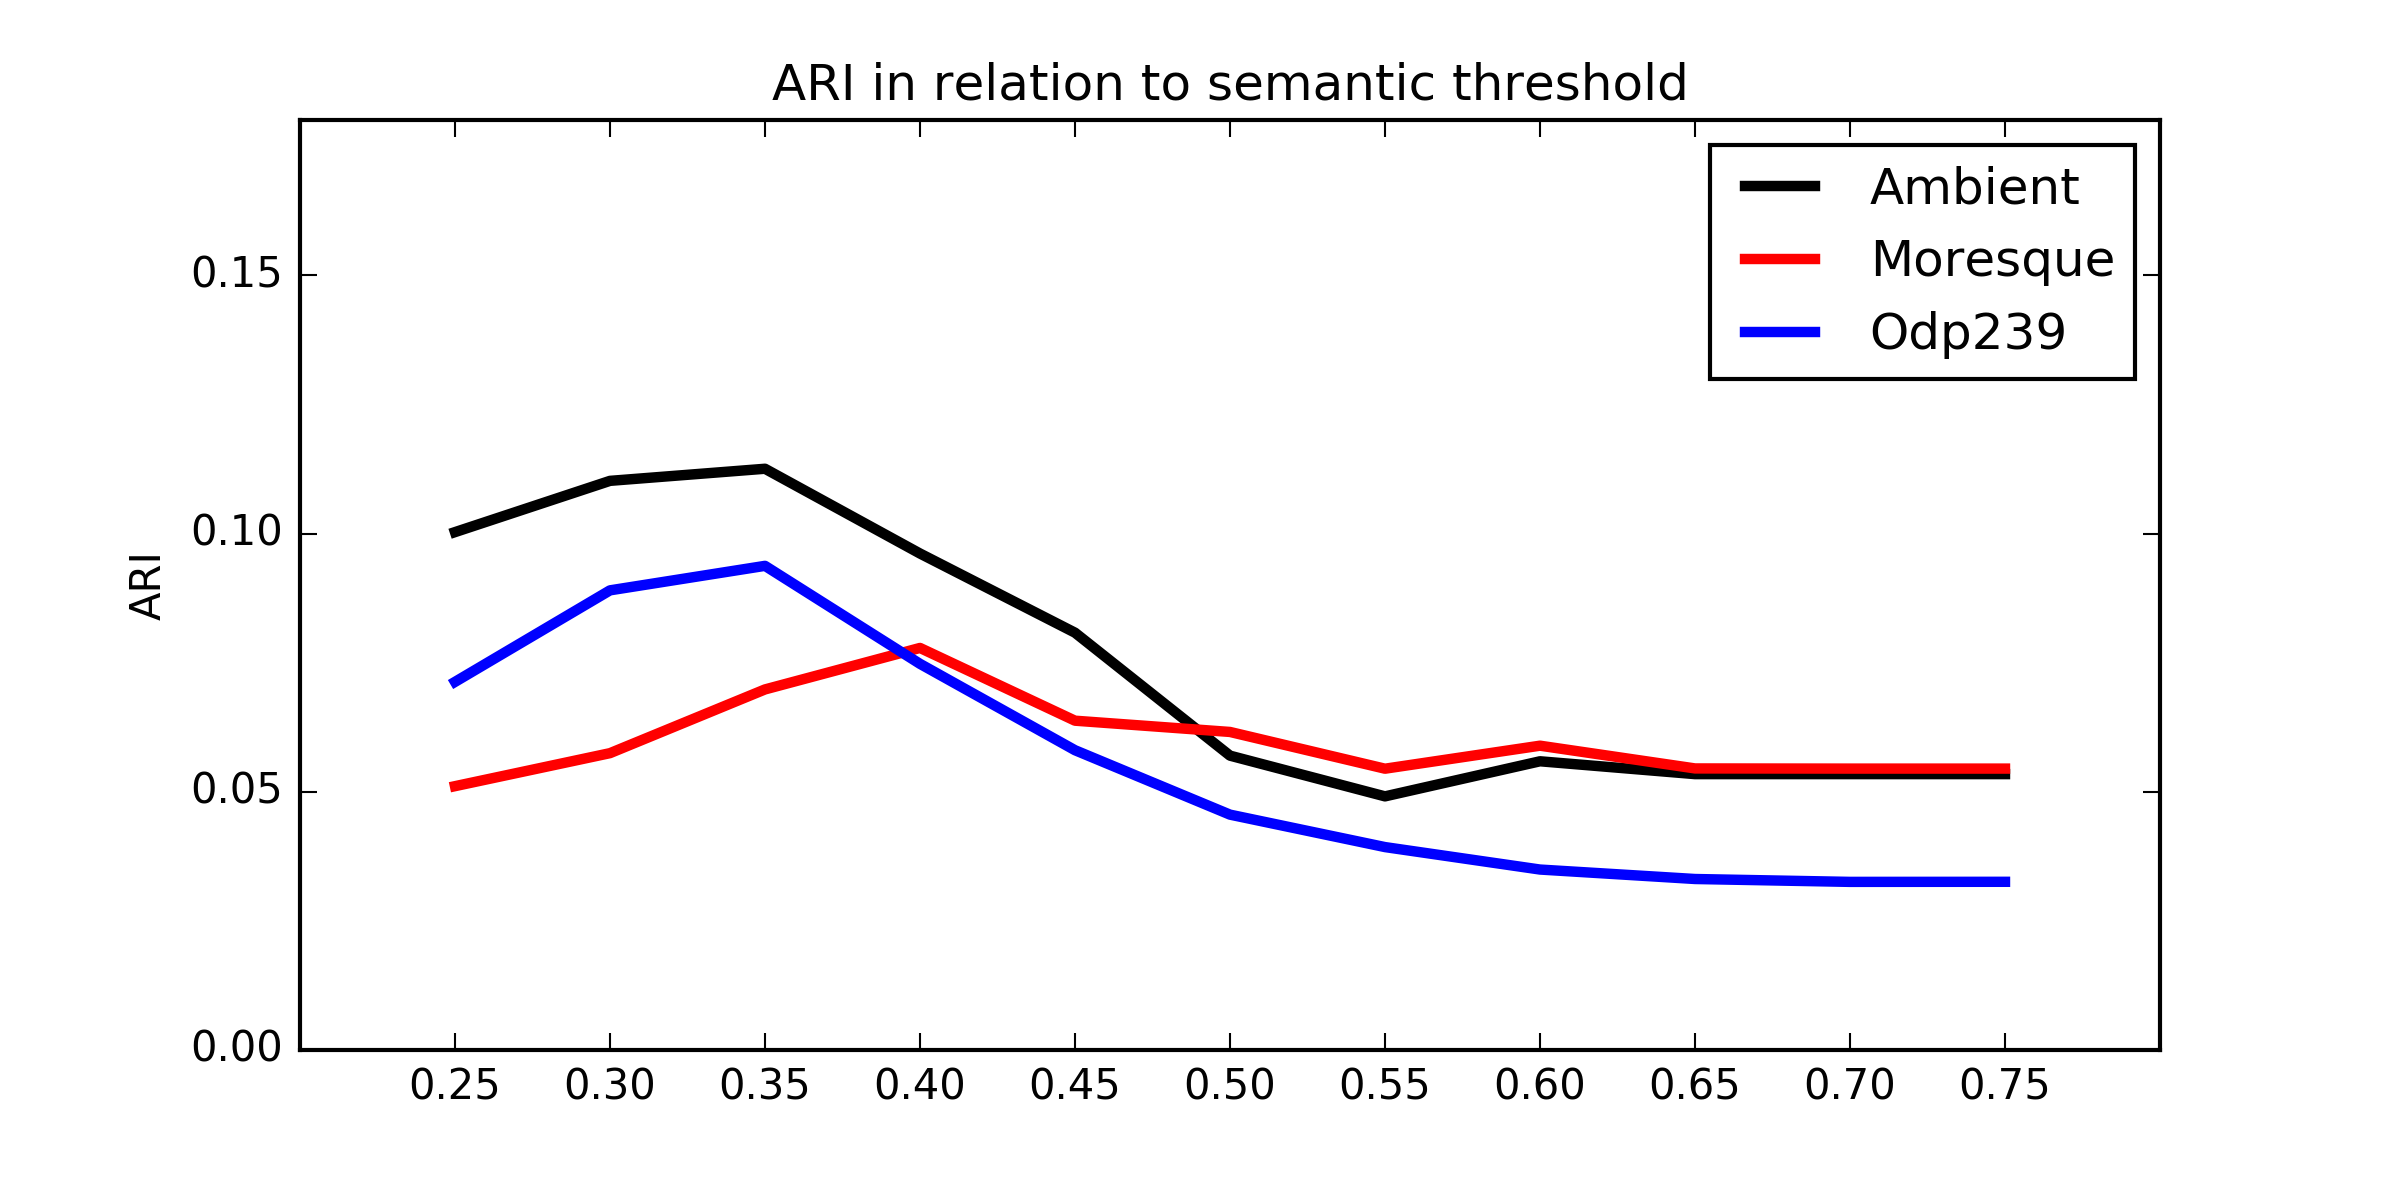
\includegraphics[width=1.0\linewidth]{Figures/sem_threshold_reult_ARI.png}
  \caption{Semantic threshold influence on Adjusted Rand Index}
  \label{fig:semparamfig2}
\end{figure}

\begin{figure}[h]
  \centering
  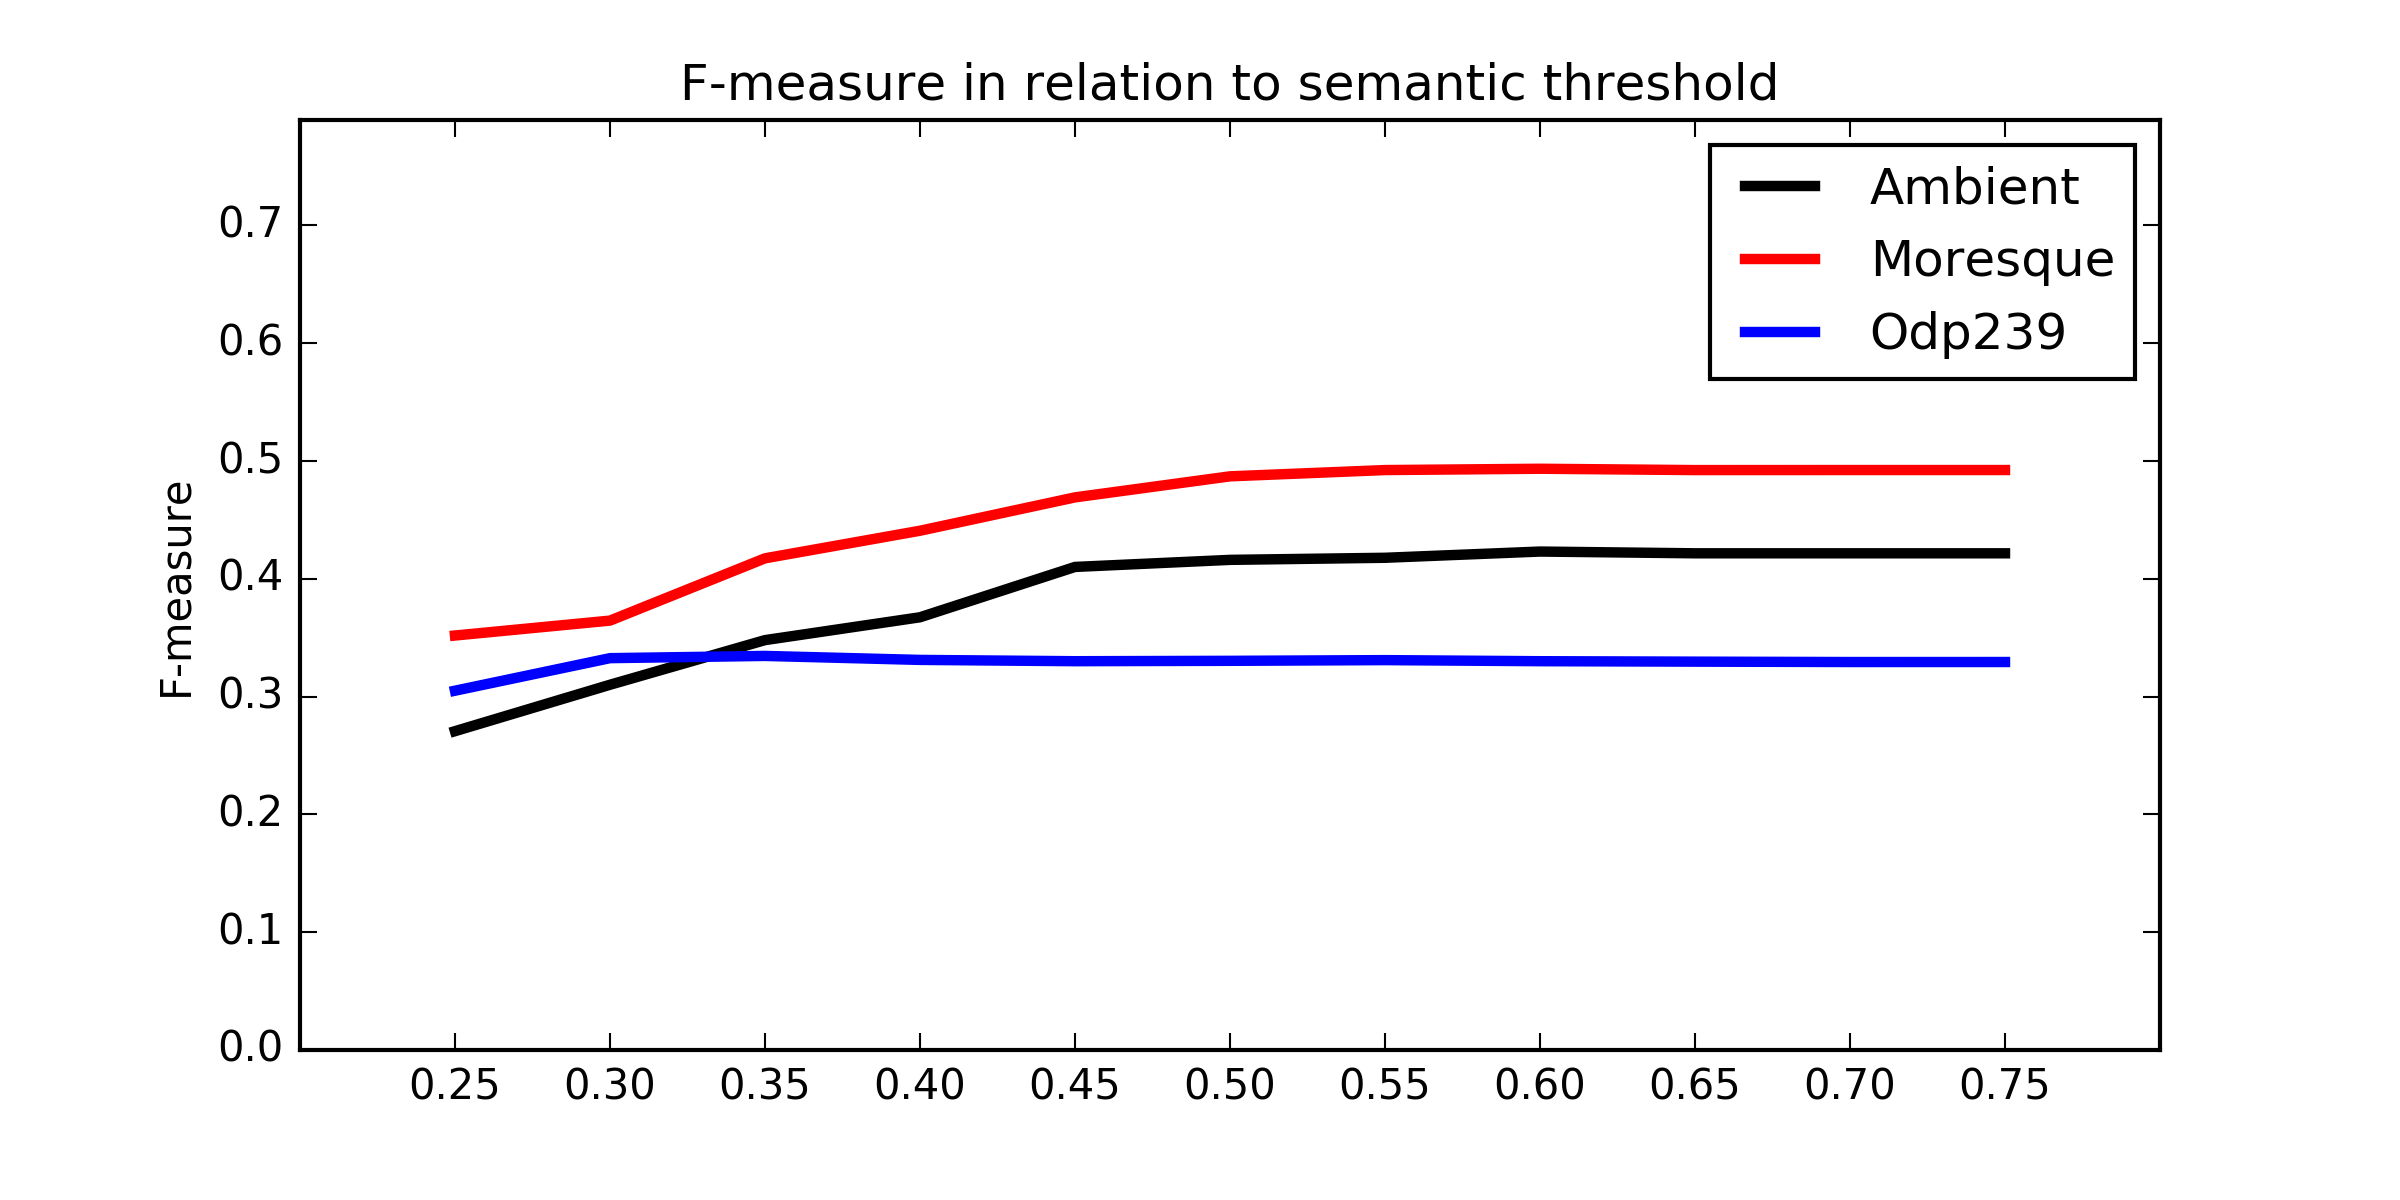
\includegraphics[width=1.0\linewidth]{Figures/sem_threshold_reult_F-measure-classic.png}
  \caption{Semantic threshold influence on \mathit{F-measure}}
  \label{fig:semparamfig3}
\end{figure}

\begin{figure}[h]
  \centering
  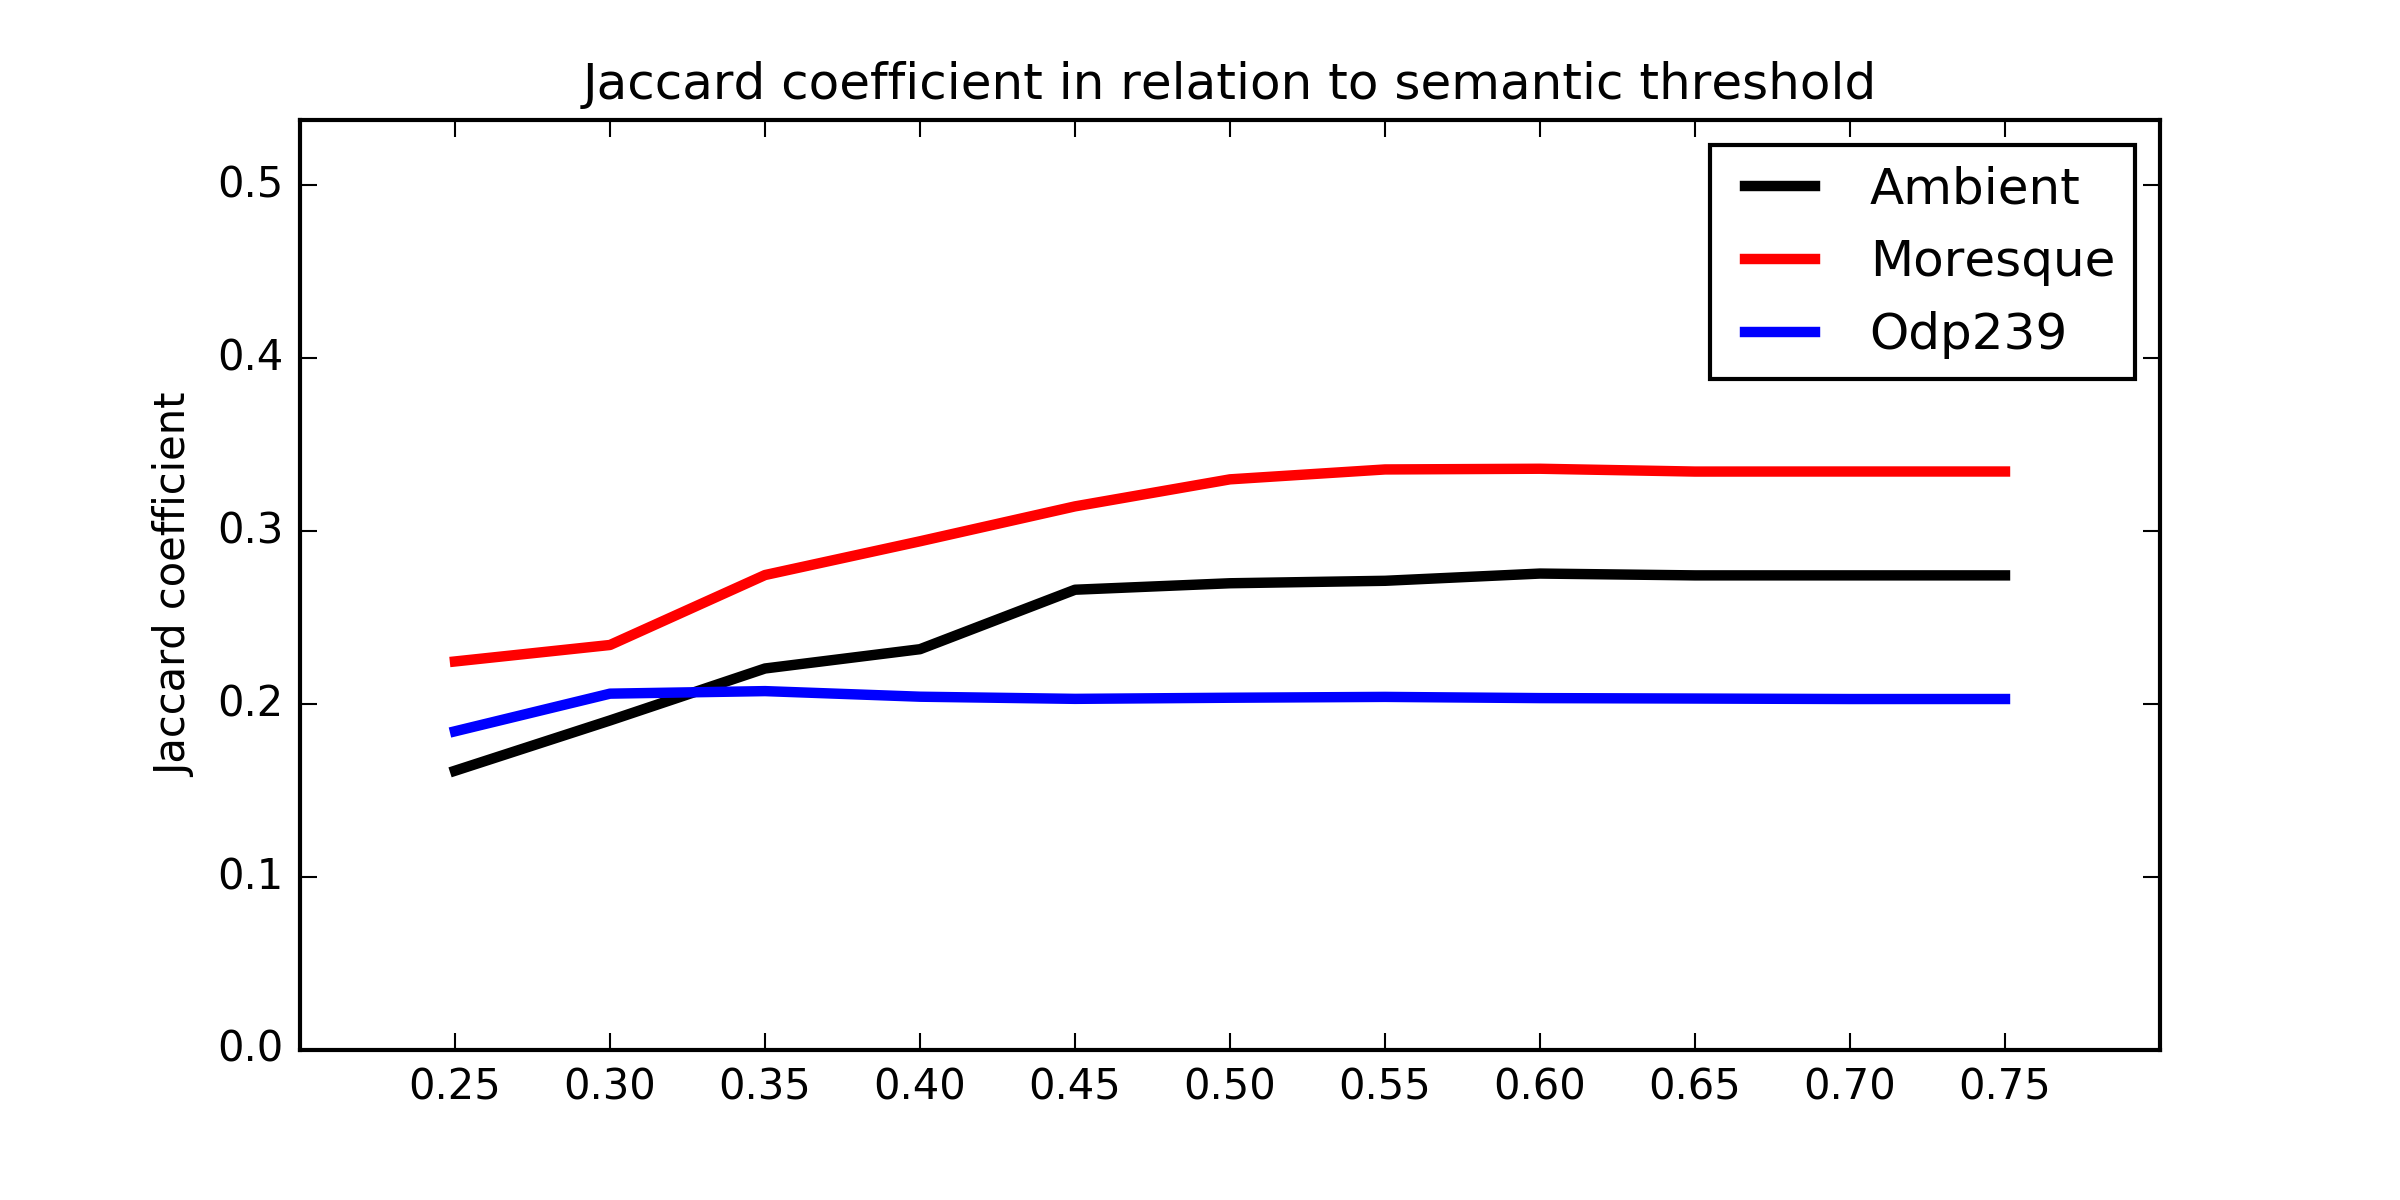
\includegraphics[width=1.0\linewidth]{Figures/sem_threshold_reult_Jaccard.png}
  \caption{Semantic threshold influence on Jaccard coefficient}
  \label{fig:semparamfig4}
\end{figure}

\begin{table}[th]
\centering
\begin{tabular}{l|rrr|rrr}
\toprule
{} & Jaccard &          &        &     ARI &          &        \\
 & Ambient & Moresque & Odp239 & Ambient & Moresque & Odp239 \\
T_{sem} &         &          &        &         &          &        \\
\midrule
0.25  &  0.1614 &   0.2246 & 0.1842 &  0.1003 &   0.0511 & 0.0713 \\
0.30  &  0.1905 &   0.2341 & 0.2060 &  0.1102 &   0.0575 & 0.0890 \\
0.35  &  0.2205 &   0.2746 & 0.2075 &  0.1126 &   0.0698 & 0.0937 \\
0.40  &  0.2317 &   0.2941 & 0.2042 &  0.0961 &   0.0779 & 0.0748 \\
0.45  &  0.2661 &   0.3143 & 0.2030 &  0.0808 &   0.0638 & 0.0580 \\
0.50  &  0.2698 &   0.3299 & 0.2036 &  0.0570 &   0.0616 & 0.0456 \\
0.55  &  0.2712 &   0.3356 & 0.2041 &  0.0491 &   0.0545 & 0.0393 \\
0.60  &  0.2754 &   0.3360 & 0.2034 &  0.0559 &   0.0589 & 0.0349 \\
0.65  &  0.2744 &   0.3344 & 0.2032 &  0.0534 &   0.0545 & 0.0331 \\
0.70  &  0.2744 &   0.3344 & 0.2029 &  0.0534 &   0.0545 & 0.0326 \\
0.75  &  0.2744 &   0.3344 & 0.2029 &  0.0534 &   0.0545 & 0.0326 \\
\bottomrule
\end{tabular}
\caption{Semantic threshold results table: Jaccard and ARI}
\label{tab:semparamtablep1}
\end{table}

\begin{table}[th]
\centering
\begin{tabular}{l|rrr|rrr}
\toprule
{} &     AMI &          &        & \mathit{F-measure-classic} &          &        \\
 & Ambient & Moresque & Odp239 &           Ambient & Moresque & Odp239 \\
T_{sem} &         &          &        &                   &          &        \\
\midrule
0.25  &  0.1552 &   0.0776 & 0.1178 &            0.2707 &   0.3519 & 0.3050 \\
0.30  &  0.1586 &   0.0795 & 0.1167 &            0.3101 &   0.3646 & 0.3327 \\
0.35  &  0.1604 &   0.0888 & 0.1315 &            0.3480 &   0.4174 & 0.3346 \\
0.40  &  0.1458 &   0.1002 & 0.1140 &            0.3674 &   0.4409 & 0.3312 \\
0.45  &  0.1181 &   0.0869 & 0.0955 &            0.4101 &   0.4692 & 0.3301 \\
0.50  &  0.0885 &   0.0770 & 0.0829 &            0.4161 &   0.4870 & 0.3304 \\
0.55  &  0.0785 &   0.0715 & 0.0772 &            0.4179 &   0.4924 & 0.3310 \\
0.60  &  0.0836 &   0.0712 & 0.0715 &            0.4232 &   0.4935 & 0.3301 \\
0.65  &  0.0807 &   0.0703 & 0.0693 &            0.4217 &   0.4924 & 0.3297 \\
0.70  &  0.0807 &   0.0702 & 0.0688 &            0.4217 &   0.4924 & 0.3294 \\
0.75  &  0.0807 &   0.0702 & 0.0688 &            0.4217 &   0.4924 & 0.3294 \\
\bottomrule
\end{tabular}
\caption{Semantic threshold results table: AMI and \mathit{F-measure}}
\label{tab:semparamtablep2}
\end{table}
\clearpage

We can see that the bahaviour for Jaccard index and \mathit{F-measure} is the monotonic growth of measures together with $T_{sem}$, contrary optimal $T_{sem}$ for Adjusted Mutual Information and Adjusted Rand Index is at lower level and decreases with $T_{sem}$ increase. From practical point of view, depending on what is an application of the algorithm (alternatively formulating it - what is the most important measure from the performance perspective), we would need to tune algorithm in a different manner.

\clearpage

\section{Third level parameters}

In the last part of parameters analysis, we will focuts on $T_k$ and $T_{other}$.

\begin{table}[th]
\centering
\begin{tabular}{lrrrr}
\toprule
{} &  AMI &  ARI &  Jaccard &  \mathit{F-measure} \\
\midrule
Ambient  & 0.35 & 0.35 &     0.60 &               0.60 \\
Moresque & 0.40 & 0.40 &     0.60 &               0.60 \\
Odp239   & 0.35 & 0.35 &     0.35 &               0.35 \\
\bottomrule
\end{tabular}
\caption{Semantic threshold value for $T_k$ and $T_{other}$ analysis}
\label{tab:heatmaplimits}
\end{table}

\begin{figure}[!htbp]
  \centering
  \subfloat[]{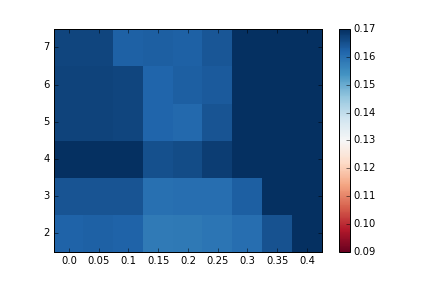
\includegraphics[width=0.33\textwidth]{Figures/heatmap_AMI_Ambient.png}}
  \hfill
  \subfloat[Moresque]{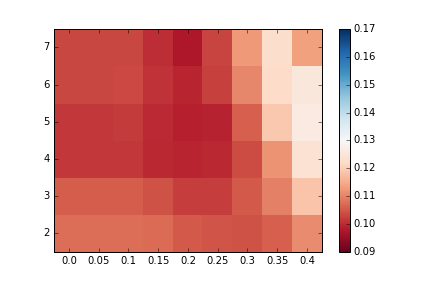
\includegraphics[width=0.33\textwidth]{Figures/heatmap_AMI_Moresque.png}}
  \hfill
  \subfloat[Odp239]{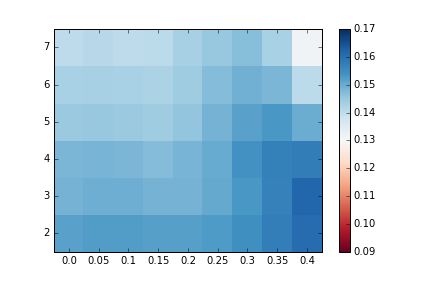
\includegraphics[width=0.33\textwidth]{Figures/heatmap_AMI_Odp239.png}}  
  \caption{Heatmap for AMI in function of $T_k$ and $T_{other}$}
  \label{fig:heatmap1}
\end{figure}

\begin{figure}[!htbp]
  \centering
  \subfloat[Ambient]{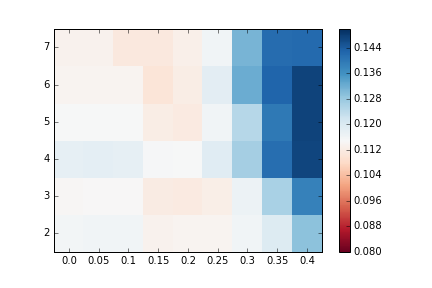
\includegraphics[width=0.33\textwidth]{Figures/heatmap_ARI_Ambient.png}}
  \hfill
  \subfloat[Moresque]{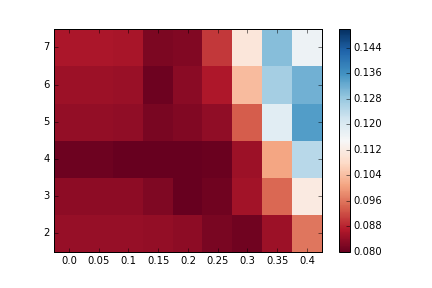
\includegraphics[width=0.33\textwidth]{Figures/heatmap_ARI_Moresque.png}}
  \hfill
  \subfloat[Odp239]{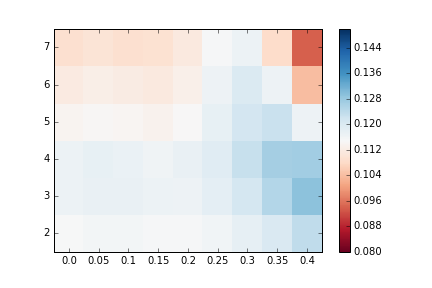
\includegraphics[width=0.33\textwidth]{Figures/heatmap_ARI_Odp239.png}}  
  \caption{Heatmap for ARI in function of $T_k$ and $T_{other}$}
  \label{fig:heatmap2}
\end{figure}

\begin{figure}[!htbp]
  \centering
  \subfloat[Ambient]{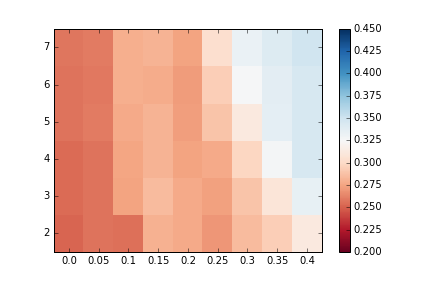
\includegraphics[width=0.33\textwidth]{Figures/heatmap_Jaccard_Ambient.png}}
  \hfill
  \subfloat[Moresque]{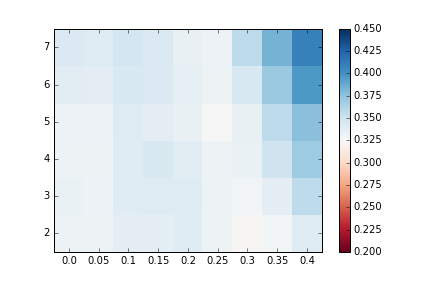
\includegraphics[width=0.33\textwidth]{Figures/heatmap_Jaccard_Moresque.png}}
  \hfill
  \subfloat[Odp239]{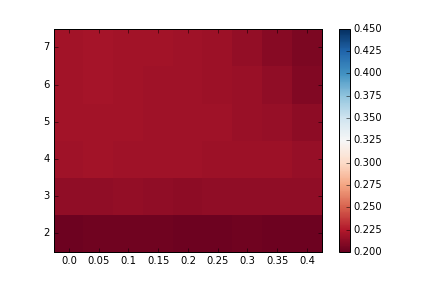
\includegraphics[width=0.33\textwidth]{Figures/heatmap_Jaccard_Odp239.png}}  
  \caption{Heatmap for Jaccard coefficient in function of $T_k$ and $T_{other}$}
  \label{fig:heatmap3}
\end{figure}

\begin{figure}[!htbp]
  \centering
  \subfloat[Ambient]{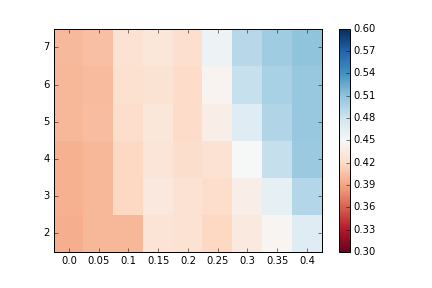
\includegraphics[width=0.33\textwidth]{Figures/heatmap_F-measure-classic_Ambient.png}}
  \hfill
  \subfloat[Moresque]{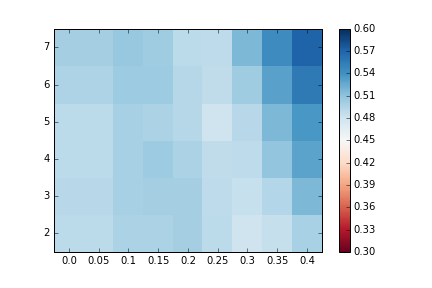
\includegraphics[width=0.33\textwidth]{Figures/heatmap_F-measure-classic_Moresque.png}}
  \hfill
  \subfloat[Odp239]{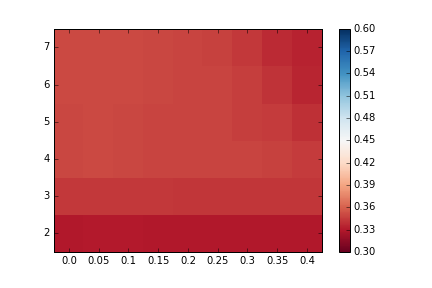
\includegraphics[width=0.33\textwidth]{Figures/heatmap_F-measure-classic_Odp239.png}}  
  \caption{Heatmap for \mathit{F-measure} in function of $T_k$ and $T_{other}$}
  \label{fig:heatmap4}
\end{figure}

In table \ref{tab:heatmaplimits} we present the value of $T_{sem}$ used for each pair of dataset and measure. The values are calculated post application of "fallback rule", described in previous section. Having the data limited to selected parameters only, we calculate the average value for each combination of $T_k$ and $T_{other}$. The results are presented in the form of heatmaps for Adjusted Mutual Information \ref{fig:heatmap1}, Adjusted Rand Index \ref{fig:heatmap2}, \mathit{F-measure} \ref{fig:heatmap3} and Jaccard index \ref{fig:heatmap4}.

First observation from heatmap analysis is the fact that regardless of measure and dataset it is always the extreme values (from the ones that were chosen for experiments) that are yielding the best results.

Heatmaps for Jaccard index and \mathit{F-measure} look very similar, having consitently best results for large values of $T_k$ and $T_{others}$. It may be associated with the fact, that both measures promote very much so called All-In-One baseline and such parameters have a tendency to put most of the documents into the "other" cluster.

For Adjusted Mutual Information and Adjusted Rand Index parameter $T_{other}$ has much larger significance than $T_k$ and the larger it is the better are results. Interesting observation is that for all the datasets $T_k$ yields best results if it is not large.

\section{Results discussion} Over 50 papers were investigated in search for possible corresponding results, which would enable solid evaluation of proposed novel document clustering algorithm (Google Scholar and other sources were searched with use of keywords AMBIENT, MORESQUE, ODP-239, Clustering, Grouping, Classification etc. in various combinations).

Used in thesis measures and datasets are largely inspired by them, although their lecture revealed many problems. The most challenging appeared to be finding a paper with experiments matching even partially a few other papers in terms of configuration of measures and datasets. Researchers tend to publish results on only a few from many available datasets (which often do not fully overlap with others) and with regard to particular measure of choice, trying to convince that entropy / Rand Index / specific \mathit{F-measure} is the most appropriate.

Moreover even after deciding on for instance AMBIENT dataset and \mathit{F-measure}, experiments might have specific implementation with many silent assumptions like for instance, that clusters smaller than 3 are not taken into account or cluster "Others" is discounted (in spite of being often majority cluster). 

Additionally when referencing to \mathit{F-measure} it is often not clear if micro or macro averaging was used and what was averaging strategy (weighted geometrically vs dedicated method). Not to mention that each  specific implementation of \mathit{F-measure} in different manner reacts to silent assumptions.  

This leads to great deal of problems with assessing if proposed in thesis novel algorithm excels. Results achieved by novel algorithm are illustrated at \ref{tab:mynovelresults}. Mind that for each cell was used different set of parameters, but this is logical in face of other researchers tuning their algorithms with regard to particular dataset and measure. 
In section dedicated to evaluation metrics it was stated that \mathit{F-measure} used is micro arithmetically averaged F1 measure in classic understanding. In similar manner as in ARI, AMI and Jaccard no silent assumptions were made and cluster "Others" is not discounted, although all clustering producing only 1 or 2 clusters are ignored for eliminating noise in data as well as from logic standpoint clustering algorithm applies fallback in such cases.

Despite all of the above effort has been made to gather results from \cite{carpineto2010optimal}, \cite{cobos2014clustering}, \cite{moreno2014easy}, \cite{acharya2014multi}, \cite{kozlowskiweb}, \cite{di2013clustering}.

Table \ref{tab:fmeasurevarious} illustrates results of \cite{carpineto2010optimal}, \cite{cobos2014clustering}, \cite{moreno2014easy}, \cite{acharya2014multi} with regard to \mathit{F-measure} although all problems listed above appear here. In table Bisecting K-means is denoted as BK and WDC-CSK BIC as BIC (BICC accordingly).

Additionally to \mathit{F-measure} from thesis standpoint evaluation of results with regard to ARI, AMI and Jaccard index is valuable. Two papers: \cite{kozlowskiweb} and \cite{di2013clustering} used them, although former performs tests only on AMBIENT and later on AMBIENT + MORESQUE. Significant difference in results shows however, that metrics were calculated in absolutely different manners (hence separation)

In \cite{kozlowskiweb} classic SRC algorithms were evaluated, namely STC, Lingo and BK (Bisecting K-means), with regard to \mathit{F-measure}, Jaccard index and Adjusted Rand Index (ARI). Results are illustrated in \ref{tab:ambientvariousmeasures}. 

In \cite{di2013clustering} various WSI-based algorithms were were evaluated, as well as a few classic ones (KeySRC, SRC, LINGO) with regard to \mathit{F-measure}, Jaccard index and Adjusted Rand Index (ARI). Results are illustrated in \ref{tab:navigliwsivariousmeasures}. 

Taking into account how algorithm behaves for various parameters it cannot be stated undoubtedly, that it excels over others, but with dose of minimized and inspected uncertainty, it visibly produces satisfactory results both in terms of data related metrics as well as informativeness, giving users meaningful cluster labels.

\vspace{1cm}

\begin{table}[th]
\centering
\begin{tabular}{l|rrrr}
\toprule
  dataset &   \rotatebox{60}{AMI} &    \rotatebox{60}{ARI} &  \rotatebox{60}{\mathit{F-measure}} &  \rotatebox{60}{Jaccard}\\
\midrule
  Ambient &        0.19 & 0.16 &   0.53 & 0.37 \\ \hline
 Moresque &        0.12 & 0.13 &     0.67 &   0.52 \\ \hline
   Odp239 &        0.17  & 0.14 &     0.36 &  0.23 \\
\bottomrule
\end{tabular}
\caption{\mathit{F-measure}, Jaccard, ARI and AMI on AMBIENT, MORESQUE and ODP-239 obtained by novel algorithm proposed in thesis}
\label{tab:mynovelresults}
\end{table}

\vspace{1cm}

\begin{table}[th]
\centering
\begin{tabular}{|c|c|c|c|} 
\toprule
\multicolumn{1}{c}{Algorithm} &  \multicolumn{3}{c}{Measure} \\ 
\midrule
 &	\mathit{F-measure} &	Jaccard	& ARI	\\
STC	& 0.53	& 0.28	& 0.23	\\
Lingo	& 0.49	& 0.3	& 0.18	\\
BK	& 0.49	& 0.12	& 0.07	\\
\bottomrule
\end{tabular}
\caption{\mathit{F-measure}, Jaccard	and ARI on AMBIENT from \cite{kozlowskiweb}}
\label{tab:ambientvariousmeasures}
\end{table}

\begin{table}[th]
\centering
\begin{tabular}{|c|c|c|c|} 
\toprule
\multicolumn{1}{c}{Algorithm} &  \multicolumn{3}{c}{Measure} \\ 
\midrule
 &	\mathit{F-measure} &	Jaccard	& ARI	\\
Curvature	& 0.6703	& 0.741	& 0.5834	\\
SquaT++(V)	& 0.6965	& 0.7569	& 0.5919	\\
SquaT++(E)	& 0.6988	& 0.7582	& 0.5939	\\
B-MST	& 0.6076	& 0.7151	& 0.6456	\\
HyperLex	& 0.6086	& 0.7205	& 0.6541	\\
Chinese Whispers	& 0.6775	& 0.7537	& 0.6425	\\
Lingo	& -0.0053	& 0.3636	& 0.1637	\\
SRC	& -0.079	& 0.3823	& 0.1496	\\
KeySRC	& 0.1434	& 0.2777	& 0.6311	\\
\bottomrule
\end{tabular}
\caption{\mathit{F-measure}, Jaccard	and ARI on AMBIENT and MORESQUE from \cite{di2013clustering}}
\label{tab:navigliwsivariousmeasures}
\end{table}

\begin{table}[th]
\centering
\begin{tabular}{|c|c|c|c|c|c|c|c|c|}
\toprule
\multicolumn{3}{c}{ODP-239} &  \multicolumn{3}{c}{MORESQUE} & \multicolumn{3}{c}{AMBIENT}\\
\midrule
BK	& \cite{acharya2014multi}	& 0.2	& BK	& \cite{acharya2014multi}	& 0.31	& 	& 	& 0	\\
BK	& \cite{cobos2014clustering}	& 0.34	& BK	& \cite{cobos2014clustering}	& 0.38	& BK	& \cite{cobos2014clustering}	& 0.45	\\
BK	& \cite{moreno2014easy}	& 0.33	& BK	& \cite{moreno2014easy}	& 0.58	& 	& 	& 0	\\
GK-means	& \cite{acharya2014multi}	& 0.36	& GK-means	& \cite{acharya2014multi}	& 0.66	& 	& 	& 0	\\
KeySRC	& \cite{carpineto2010optimal}	& 0.29	& 	& 	& 0	& 	& 	& 0	\\
Liingo	& \cite{acharya2014multi}	& 0.27	& Lingo	& \cite{acharya2014multi}	& 0.32	& 	& 	& 0	\\
Lingo	& \cite{carpineto2010optimal}	& 0.31	& 	& 	& 0	& 	& 	& 0	\\
Lingo	& \cite{carpineto2010optimal}	& 0.27	& 	& 	& 0	& 	& 	& 0	\\
Lingo	& \cite{cobos2014clustering}	& 0.41	& Lingo	& \cite{cobos2014clustering}	& 0.5	& Lingo	& \cite{cobos2014clustering}	& 0.58	\\
Lingo	& \cite{moreno2014easy}	& 0.33	& Lingo	& \cite{moreno2014easy}	& 0.6	& 	& 	& 0	\\
MOO-clus	& \cite{acharya2014multi}	& 0.38	& MOO-clus	& \cite{acharya2014multi}	& 0.67	& 	& 	& 0	\\
OPTIMSRC	& \cite{acharya2014multi}	& 0.31	& 	& 	& 0	& 	& 	& 0	\\
OPTIMSRC	& \cite{carpineto2010optimal}	& 0.31	& 	& 	& 0	& 	& 	& 0	\\
STC	& \cite{acharya2014multi}	& 0.32	& STC	& \cite{acharya2014multi}	& 0.45	& 	& 	& 0	\\
STC	& \cite{cobos2014clustering}	& 0.41	& STC	& \cite{cobos2014clustering}	& 0.57	& STC	& \cite{cobos2014clustering}	& 0.55	\\
STC	& \cite{moreno2014easy}	& 0.33	& STC	& \cite{moreno2014easy}	& 0.6	& 	& 	& 0	\\
STC-LINGO	& \cite{acharya2014multi}	& 0.36	& STC-LINGO	& \cite{acharya2014multi}	& 0.56	& 	& 	& 0	\\
BBIC	& \cite{cobos2014clustering}	& 0.46	& BBBIC	& \cite{cobos2014clustering}	& 0.49	& BBIC	& \cite{cobos2014clustering}	& 0.62	\\
BBIC	& \cite{cobos2014clustering}	& 0.45	& BBIC	& \cite{cobos2014clustering}	& 0.48	& BIC	& \cite{cobos2014clustering}	& 0.6	\\
\bottomrule
\end{tabular}
\caption{\mathit{F-measure} metric on AMBIENT, MORESQUE and ODP-239 achieved by various algorithms from \cite{carpineto2010optimal}, \cite{cobos2014clustering}, \cite{moreno2014easy}, \cite{acharya2014multi}}
\label{tab:fmeasurevarious}
\end{table}

\chapter{Summary} Following chapter focuses on concluding thesis by discussing results and proposal of further work. Additionally performs assessment whether initial objectives were completed and original contributions were delivered.

\section{Conclusions} Novel DC algorithm using external knowledge sources for semantic relations (word2vec with SG model trained on Google News corpus) and advanced NLP techniques was proposed, implemented and evaluated. Implementation of proposed novel DC algorithm was fully documented. Together with instruction of usage and notes from creation process it can be used for reproducible research purposes.

Reproducible research rules were formulated after observing way of conducting research in DC domain and whole thesis was created applying them in practice.

Thorough literature study was conducted on subject of DC and SRC. Theory crucial for understanding the most important aspects of thesis, quoted articles and state of the art methods was discussed.

Technicalities of conducted research and applied engineering techniques were covered, emphasising their usage for sake of successfully implementing proposed reproducible research rules. Tool and techniques used in this process were presented in dedicated chapter, allowing further investigation.

Evaluation of novel DC algorithm in terms of efficiency and performance on proposed datasets, with suggested measures, in comparison to selected algorithms, has shown that in comparison to other WSI methods it produces satisfactory results and can be successfully applied in various clustering scenarios.

\section{Further work} After conducting experiments with semantic relatedness calculated with word2vec with SG model trained on Google News corpus, that would be great to see how other word2vec models would perform. Especially promising seems the one trained on FreeBase provided by Google as clustering encyclopedic and ambiguous queries should benefit from more adequate character of training set and data source.

EasyESA and other semantic relatedness strategies seem to be very promising and could be investigated.

Muti-objective Optimization with use of WSI and semantic relatedness based algorithms (among them novel proposed in thesis) as ensembles seems to be interesting subject of further research.

%% ----------------------------------------------------------------
% Now begin the Appendices, including them as separate files

%\addtocontents{toc}{\vspace{2em}} % Add a gap in the Contents, for aesthetics

%\appendix % Cue to tell LaTeX that the following 'chapters' are Appendices

%\input{Appendices/AppendixA}	% Appendix Title

%\input{Appendices/AppendixB} % Appendix Title

%\input{Appendices/AppendixC} % Appendix Title

%\addtocontents{toc}{\vspace{2em}} % Add a gap in the Contents, for aesthetics
%\backmatter

%% ----------------------------------------------------------------
\label{Bibliography}
%\lhead{\emph{Bibliography}} % Change the left side page header to "Bibliography"
\bibliographystyle{unsrtnat} % Use the "unsrtnat" BibTeX style for formatting the Bibliography
\bibliography{Bibliography} % The references (bibliography) information are stored in the file named "Bibliography.bib"

\end{document} % The End
%% ----------------------------------------------------------------